\documentclass[11pt,a4paper]{article}

% --- Essential Packages ---
\usepackage[margin=1in]{geometry}
\usepackage{fontspec}
\usepackage[english]{babel}
\usepackage{amsmath,amssymb,amsfonts}
\usepackage{booktabs}
\usepackage{tabularx}
\usepackage{array}
\usepackage{xcolor}
\usepackage{listings}
\usepackage{tikz}
\usepackage{subcaption}
\usetikzlibrary{shapes.geometric, arrows.meta, positioning}
\usepackage{hyperref}

% --- Font Configuration (Times New Roman Mapping) ---
\babelfont{rm}{Times New Roman}

% --- Color Palette ---
\definecolor{primary}{RGB}{20, 35, 60}
\definecolor{secondary}{RGB}{45, 85, 125}
\definecolor{accent}{RGB}{180, 50, 30}
\definecolor{codebg}{RGB}{245, 247, 250}
\definecolor{codeframe}{RGB}{200, 210, 220}

% --- Hyperlink Setup ---
\hypersetup{
    colorlinks=true,
    linkcolor=secondary,
    citecolor=secondary,
    urlcolor=secondary
}

% --- Listing Setup ---
\lstset{
    language=Python,
    backgroundcolor=\color{codebg},
    frame=single,
    rulecolor=\color{codeframe},
    basicstyle=\small\ttfamily,
    keywordstyle=\color{secondary}\bfseries,
    stringstyle=\color{accent},
    commentstyle=\color{gray}\itshape,
    breaklines=true,
    showstringspaces=false,
    tabsize=4
}

% --- Document Metadata ---
\title{\textbf{\Large Phase 1 Technical Report: Problem Formulation, Data Understanding, and Quality Audit}\\
\large NYC Yellow Taxi Hourly Demand Forecasting \& Congestion Pricing Impact Analysis (2025)}
\author{\textbf{Data Analysis Course Project} (Fall 2026 / 1405)\\
Track A: NYC TLC Structured Time-Series Analysis}
\date{October 27, 2026}

\begin{document}

\maketitle

\begin{abstract}
This report presents Phase 1 of the NYC Yellow Taxi demand forecasting project for the full calendar year 2025. Leveraging a local DuckDB analytical engine operating directly over 12 monthly Parquet files (~48.7 million trip records), we execute a comprehensive data structure and data quality audit. We formalize the operational decision problem—assisting fleet operators in pre-positioning vehicles across 265 taxi zones and evaluating the newly enacted 2025 Central Business District (CBD) congestion fee—by establishing the spatio-temporal aggregation unit $(z, t) \in \text{Zone} \times \text{Hour}$. Our audit reveals complete temporal continuity with zero null value records across core fields, while quantifying specific physical and financial anomalies: 546,304 non-positive duration trips (1.12\%), 1,402,958 zero-distance trips (2.88\%), and 2,848,620 negative fare entries (5.85\%). Finally, we define a strict temporal split protocol (Train: Jan--Sep 2025; Test: Oct--Dec 2025) to prevent future data leakage and outline baseline models for subsequent implementation phases.
\end{abstract}

\section{Problem Definition and Motivation}
Taxicab demand in dense urban environments exhibits high spatial variance and non-stationary temporal dynamics. Following the 2025 implementation of the New York City Central Business District (CBD) congestion pricing fee (\texttt{cbd\_congestion\_fee}), fleet managers and independent operators face increased operational overhead and altered passenger booking behavior.

The core motivation of this project is to assist vehicle fleet managers in dynamically pre-positioning taxicabs across official NYC Taxi and Limousine Commission (TLC) zones. By accurately forecasting hourly trip originations per zone, dispatchers can minimize idle cruising time, reduce passenger wait times, and optimize fleet allocation under new congestion fee structures.

\section{Related Work}
Short-term urban passenger demand forecasting traditionally relies on historical rolling averages and Auto-Regressive Integrated Moving Average (ARIMA) models. Recent advances employ non-linear gradient-boosted decision trees (e.g., LightGBM, XGBoost) and spatio-temporal graph neural networks. In the context of NYC TLC datasets, prior literature emphasizes the necessity of strictly preserving temporal order during model validation to avoid look-ahead bias and spurious performance metrics.

\section{Data and Data Quality}

\subsection{Dataset Overview}
The primary dataset consists of the official NYC Yellow Taxi trip records for the entire calendar year 2025 (January 1, 2025 -- December 31, 2025), partitioned into 12 monthly Parquet files stored locally in \texttt{data/raw/}. Spatial reference lookups (\texttt{taxi\_zone\_lookup.csv}) and zone boundary shapefiles (\texttt{taxi\_zones.shp}) are stored in \texttt{data/spatial/}.

\subsection{Structural Audit}
Using an in-memory DuckDB query engine, we processed all 12 Parquet files in a single unified operation without memory overflow. Table~\ref{tab:schema} lists the complete schema of the 2025 dataset, comprising 20 columns.

\begin{table}[htbp]
\centering
\caption{NYC Yellow Taxi 2025 Dataset Schema and Variable Categorization}
\label{tab:schema}
\small
\begin{tabularx}{\textwidth}{llXX}
\toprule
\textbf{Column Name} & \textbf{Data Type} & \textbf{Category} & \textbf{Description / Role} \\
\midrule
\texttt{VendorID} & INTEGER & Categorical ID & TPEP provider code \\
\texttt{tpep\_pickup\_datetime} & TIMESTAMP & Datetime Variable & Trip start time (Meter engaged) \\
\texttt{tpep\_dropoff\_datetime} & TIMESTAMP & Datetime Variable & Trip end time (Meter disengaged) \\
\texttt{passenger\_count} & BIGINT & Numeric & Driver-entered passenger count \\
\texttt{trip\_distance} & DOUBLE & Continuous Numeric & Elapsed trip distance (miles) \\
\texttt{RatecodeID} & BIGINT & Categorical ID & Final rate code in effect \\
\texttt{store\_and\_fwd\_flag} & VARCHAR & Flag & Memory buffer transmission flag \\
\texttt{PULocationID} & INTEGER & Spatial ID & Pickup TLC Taxi Zone ID ($1..263$) \\
\texttt{DOLocationID} & INTEGER & Spatial ID & Dropoff TLC Taxi Zone ID ($1..263$) \\
\texttt{payment\_type} & BIGINT & Categorical & Payment method (1=Credit, 2=Cash) \\
\texttt{fare\_amount} & DOUBLE & Financial Numeric & Metered time-and-distance fare \\
\texttt{extra} & DOUBLE & Financial Numeric & Miscellaneous extras and surcharges \\
\texttt{mta\_tax} & DOUBLE & Financial Numeric & \$0.50 MTA state tax \\
\texttt{tip\_amount} & DOUBLE & Financial Numeric & Credit card tip amount \\
\texttt{tolls\_amount} & DOUBLE & Financial Numeric & Total bridge/tunnel tolls \\
\texttt{improvement\_surcharge} & DOUBLE & Financial Numeric & \$0.30 improvement surcharge \\
\texttt{total\_amount} & DOUBLE & Financial Numeric & Total charge to passenger \\
\texttt{congestion\_surcharge} & DOUBLE & Financial Numeric & Standard congestion fee \\
\texttt{Airport\_fee} & DOUBLE & Financial Numeric & Airport pickup fee \\
\texttt{cbd\_congestion\_fee} & DOUBLE & Financial Numeric & \textbf{New 2025 CBD Congestion Pricing Fee} \\
\bottomrule
\end{tabularx}
\end{table}

\subsection{Spatial Data Structure and Schema Audit}
To support spatial aggregations, zone-level demand forecasting, and geographic visualizations, we conducted a structural audit of the spatial reference files stored in \texttt{data/spatial/}.

\subsection{Taxi Zone Lookup Table (\texttt{taxi\_zone\_lookup.csv})}
The lookup table maps numerical taxi zone identifiers to descriptive geographic attributes, comprising 265 total records and 4 columns, as detailed in Table~\ref{tab:lookup_schema}.

\begin{table}[htbp]
\centering
\caption{Taxi Zone Lookup Table Schema (\texttt{taxi\_zone\_lookup.csv})}
\label{tab:lookup_schema}
\small
\begin{tabularx}{\textwidth}{llXX}
\toprule
\textbf{Column Name} & \textbf{Data Type} & \textbf{Category} & \textbf{Description / Role} \\
\midrule
\texttt{LocationID} & INTEGER & Primary Identifier & Unique zone identifier ($1..265$) \\
\texttt{Borough} & VARCHAR & Categorical & NYC Borough name (Manhattan, Queens, etc.) \\
\texttt{Zone} & VARCHAR & Descriptive & Neighborhood or specific zone name \\
\texttt{service\_zone} & VARCHAR & Categorical & Service zone classification (Yellow Zone, Boro Zone, etc.) \\
\bottomrule
\end{tabularx}
\end{table}

\subsection{Taxi Zones Spatial File (\texttt{taxi\_zones.shp})}
The spatial vector dataset provides polygon boundaries corresponding to the taxi zones (stored as an ESRI Shapefile bundle with CRS EPSG:2263), comprising 263 distinct polygon records and 7 attributes, as listed in Table~\ref{tab:spatial_schema}.

\begin{table}[htbp]
\centering
\caption{Taxi Zones Spatial Vector Schema (\texttt{taxi\_zones.shp})}
\label{tab:spatial_schema}
\small
\begin{tabularx}{\textwidth}{llXX}
\toprule
\textbf{Column Name} & \textbf{Data Type} & \textbf{Category} & \textbf{Description / Role} \\
\midrule
\texttt{OBJECTID} & INTEGER & Identifier & ESRI object feature identifier \\
\texttt{Shape\_Leng} & DOUBLE & Numeric Metric & Perimeter length of the zone polygon \\
\texttt{Shape\_Area} & DOUBLE & Numeric Metric & Area of the zone polygon \\
\texttt{zone} & VARCHAR & Descriptive & Neighborhood zone name matching lookup table \\
\texttt{LocationID} & INTEGER & Spatial ID / Foreign Key & TLC Taxi Zone ID linking to lookup and trips \\
\texttt{borough} & VARCHAR & Categorical & Borough name classification \\
\texttt{geometry} & GEOMETRY & Spatial Data Type & Polygon / MultiPolygon boundary coordinates (EPSG:2263) \\
\bottomrule
\end{tabularx}
\end{table}

\subsection{Table and Spatial Relationships}
The trip records link dynamically to the spatial reference files using \texttt{PULocationID} and \texttt{DOLocationID} as foreign keys that join against the primary key \texttt{LocationID} in both the lookup table and the spatial geometry shapefile.

\subsection{Data Quality Quantification and Decisions}
The audit evaluated $48,722,602$ raw trip records. Table~\ref{tab:quality_audit} details the findings for missing values, impossible physical measurements, and administrative anomalies, along with the corresponding handling strategy.

\begin{table}[htbp]
\centering
\caption{Data Quality Audit Metrics and Treatment Decisions (Full Year 2025)}
\label{tab:quality_audit}
\tiny
\begin{tabularx}{\textwidth}{lrrX}
\toprule
\textbf{Metric / Anomaly Category} & \textbf{Count} & \textbf{\% of Total} & \textbf{Initial Treatment Decision} \\
\midrule
Total Raw Trips & 48,722,602 & 100.00\% & Baseline dataset population \\
Missing Pickup Timestamps & 0 & 0.00\% & None required (100\% complete) \\
Missing Dropoff Timestamps & 0 & 0.00\% & None required (100\% complete) \\
Unknown Pickup Location (\texttt{PULocationID = 264}) & 80,873 & 0.17\% & \textbf{Filter Out}: Unmapped geographic pickup coordinates \\
Outside NYC Pickup Location (\texttt{PULocationID = 265}) & 22,170 & 0.05\% & \textbf{Filter Out}: Excluded for internal origin demand modeling \\
Unknown Dropoff Location (\texttt{DOLocationID = 264}) & 105,193 & 0.22\% & \textbf{Filter Out}: Unmapped geographic dropoff coordinates \\
Outside NYC Dropoff Location (\texttt{DOLocationID = 265}) & 219,073 & 4.49\% & \textbf{Conditional Retention}: Retained up to 200 miles for out-of-city flow metrics \\
Missing Distance / Fare Fields & 0 & 0.00\% & None required (100\% complete) \\
\midrule
Invalid Duration ($\le 0$ min or $> 240$ min) & 563,024 & 1.16\% & \textbf{Filter Out}: Clock reset, meter left running, or cancelled trips \\
Invalid Trip Distance (Intra $>100$mi or Out $>200$mi) & 2,429 & 0.005\% & \textbf{Filter Out}: Extreme spatial anomalies and GPS satellite jumps \\ 
Zero Trip Distance ($d = 0$ mi) & 1,402,958 & 2.88\% & \textbf{Filter Out}: Stationary meter runs / cancellations \\
Invalid Average Speed ($v > 80$ mph) & 560,004 & 1.15\% & \textbf{Filter Out}: Telemetry errors and GPS coordinate displacement \\
Micro-Trip Speed Artifacts ($\Delta t < 1$ min, $v > 70$ mph) & 8,543 & 0.018\% & \textbf{Filter/Nullify}: Timestamp jitter and GPS rounding glitches \\
Negative Fare Amount ($f < \$0$) & 2,848,620 & 5.85\% & \textbf{Filter Out}: Dispute voids, chargebacks, system tests \\
Invalid Passenger Count ($<0$ or $>9$ or \texttt{null}) & 11,611,894 & 23.83\% & \textbf{Retain As-Is}: Retained without imputation to prevent data loss. \\
\bottomrule
\end{tabularx}
\end{table}

\subsubsection{Rationale for Data Quality Treatment Decisions}
To maintain data integrity and prevent distortion in our spatio-temporal demand forecasting models, we established explicit treatment protocols for each identified anomaly category across the $48,722,602$ raw records. The individual rationales and references to representative sample records are structured as follows:

\begin{itemize}
    \item \textbf{Missing Timestamps and Spatial Location IDs ($0$ records, $0.00\%$):} 
    \textit{Decision: Retain All.} 
    \textit{Rationale:} The dataset exhibited complete structural integrity for core operational fields. Because our fundamental unit of analysis is defined by pickup location and timestamp $(z, t)$, having complete coverage in these fields ensures that no records are dropped due to missing spatial keys, eliminating potential sample selection bias at the initial ingestion stage.

    \item \textbf{Invalid Durations ($\le 0$ minutes or $> 240$ minutes, $563,024$ records, $1.16\%$):} 
    \textit{Decision: Filter Out.} 
    \textit{Rationale:} A physical taxicab trip must occupy a realistic time interval ($0 < \Delta t \le 240$ minutes). Records where dropoff precedes pickup or excessive durations exceeding $4$ hours occur indicate GPS logging latency, device clock resets, or meters left running indefinitely while parked. As illustrated in Table~\ref{tab:sample_duration}, several records exhibit durations over $1,400$ minutes ($\sim 24$ hours) for short trips under $7$ miles, confirming forgotten meters. Retaining these anomalies would severely corrupt vehicle speed calculations and duration-based features.
    
    \item \textbf{Invalid Trip Distances (Intra-city $>100$ mi or Out-of-city $>200$ mi, $2,429$ records, $0.005\%$):} 
    \textit{Decision: Filter Out.} 
    \textit{Rationale:} While standard intra-city trips are capped at $100$ miles to eliminate spatial outliers, legitimate regional long-haul journeys terminating outside NYC (\texttt{DOLocationID = 265}) are accommodated with an extended ceiling of $200$ miles to preserve authentic interstate economic flows. Records exceeding these conditional thresholds represent severe GPS tracking errors and system telemetry glitches. As shown in Table~\ref{tab:sample_distance}, multiple records log distances exceeding $1,000$ to $4,000$ miles for $10$-minute trips, resulting in implausible speeds over $4,000$ mph.

    \item \textbf{Zero-Distance Trips ($d = 0$ miles, $1,402,958$ records, $2.88\%$):} 
    \textit{Decision: Filter Out.} 
    \textit{Rationale:} While passengers may occasionally cancel a trip immediately after entering a taxi, zero-distance records predominantly reflect stationary meter testing, administrative diagnostics, or false starts. Table~\ref{tab:sample_zerodist} demonstrates that these trips typically last under $3$ minutes with identical pickup and dropoff zones while still incurring base fares. Because our spatial aggregation relies on movement across taxi zones, stationary logs distort spatial origin-destination demand densities.

    \item \textbf{Invalid Average Speeds ($v > 70$ mph, $560,004$ records, $1.15\%$):} 
    \textit{Decision: Filter Out.} 
    \textit{Rationale:} Municipal yellow cabs operating within urban street grids and regional highways cannot physically or legally sustain average speeds exceeding $80$ mph. As documented in Table~\ref{tab:sample_speed}, extreme cases record speeds ranging from $89$ mph up to $1,577$ mph over sub-minute intervals (e.g., traveling $9.20$ miles in $21$ seconds). These outliers stem from severe GPS satellite coordinate jumps and timestamp desynchronization, which would severely distort velocity profiling and travel-time estimation.

    \item \textbf{Micro-Trip Speed Artifacts ($\Delta t < 1$ min, $v > 80$ mph, $8,543$ records, $0.018\%$):} 
    \textit{Decision: Filter Out / Conditional Nullification.} 
    \textit{Rationale:} A subset of short-duration trips ($\Delta t < 1.0$ minute) featuring non-zero distance yields mathematically unstable, exaggerated velocity spikes due to timestamp rounding and high-resolution GPS clock jitter. While standard upper-speed bounds catch many of these, explicitly quantifying these $8,543$ micro-trip artifacts ensures they are handled via conditional kinematic filtering (Option 3)—either nullifying their speed derivatives or filtering them out during the Phase 2 data preparation pipeline to preserve kinematic integrity without sacrificing volume unnecessarily.

    \item \textbf{Negative Fares ($f < \$0$, $2,848,620$ records, $5.85\%$):} 
    \textit{Decision: Filter Out.} 
    \textit{Rationale:} Negative fare amounts do not represent legitimate passenger transactions; rather, they correspond to credit card chargebacks, fare dispute reversals, or system administrative adjustments. Table~\ref{tab:sample_negfare} highlights typical negative fare entries (e.g., $-\$3.00$ to $-\$24.00$) for short intra-Manhattan journeys. Including them would severely distort financial summaries and bias regression models exploring fare-demand relationships.

    \item \textbf{Unrecorded or Missing Passenger Counts ($11,611,894$ records, $23.83\%$):} 
    \textit{Decision: Retain As Is.} 
    \textit{Rationale:} Approximately $23.83\%$ of raw records exhibited missing (\texttt{NULL} / \texttt{<NA>}) passenger counts due to driver omission or meter logging habits. As detailed in Table~\ref{tab:sample_passengers}, these records represent completely valid commercial trips with normal durations, distances, and fares. Deleting them would cause severe attrition in spatio-temporal trip volume aggregations; hence, they are retained in their native state without artificial imputation.
    
    \item \textbf{Unknown and Outside NYC Locations (\texttt{LocationID = 264, 265}):} 
    \textit{Decision: Filter Out / Conditional Retention.} 
    \textit{Rationale:} Zone ID $264$ designates ``Unknown'' unmapped spatial areas and is filtered out entirely, as shown in Table~\ref{tab:sample_locations}. Zone ID $265$ represents locations outside official TLC zones; trips originating outside NYC (\texttt{PULocationID = 265}, $22,170$ records) are excluded to prevent distortion in origin demand modeling, whereas trips terminating outside NYC are retained up to $200$ miles to maintain accurate financial and out-commuter flow metrics.
\end{itemize}

\subsubsection{Summary of Cleansing Impact:}
Collectively, this rigorous filtering protocol removes $4,707,394$ anomalous records ($\approx 9.66\%$ of the total raw volume), leaving a pristine, high-fidelity baseline population of \textbf{$44,015,208$ valid trips} dedicated for downstream spatio-temporal aggregation and hourly demand forecasting.

\subsection{Empirical Examples of Identified Anomalies}
To provide concrete verification of the data quality audit, representative samples from each identified anomaly category are documented in Tables~\ref{tab:sample_duration}--\ref{tab:sample_speed} below.

\begin{table}[htbp]
\centering
\caption{Sample Records: Invalid or Excessive Duration ($\Delta t > 4$h or $\le 0$ min)}
\label{tab:sample_duration}
\tiny
\begin{tabularx}{\textwidth}{l l r r r r r X X}
\toprule
\textbf{Pickup Time} & \textbf{Dropoff Time} & \textbf{Dur} & \textbf{Dist} & \textbf{Fare} & \textbf{Speed} & \textbf{Pass} & \textbf{PU Zone} & \textbf{DO Zone} \\
\midrule
2025-01-01 01:26:00 & 2025-01-02 01:22:08 & 1436.13 & 7.06 & \$37.30 & 0.29 & 1 & Murray Hill & Boerum Hill \\
2025-01-01 00:27:08 & 2025-01-02 00:00:00 & 1412.87 & 5.72 & \$25.40 & 0.24 & 1 & Kips Bay & Brooklyn Heights \\
2025-01-01 00:18:22 & 2025-01-02 00:00:00 & 1421.63 & 1.12 & \$17.00 & 0.05 & 1 & Clinton West & Clinton East \\
2025-01-01 02:01:56 & 2025-01-02 01:17:14 & 1395.30 & 0.71 & \$8.60 & 0.03 & 4 & West Chelsea/Hudson Yards & East Chelsea \\
2025-01-01 01:31:10 & 2025-01-02 01:19:44 & 1428.57 & 0.73 & \$6.50 & 0.03 & 1 & Union Sq & East Village \\
2025-01-01 01:48:26 & 2025-01-02 01:41:57 & 1433.52 & 0.99 & \$8.60 & 0.04 & 2 & Midtown North & Lincoln Square West \\
2025-01-01 01:45:26 & 2025-01-01 11:29:42 & 584.27 & 0.56 & \$6.50 & 0.06 & 1 & Central Harlem & Queensbridge/Ravenswood \\
2025-01-01 01:09:24 & 2025-01-02 01:06:27 & 1437.05 & 3.32 & \$21.20 & 0.14 & 1 & Upper West Side North & Sutton Place/Turtle Bay North \\
2025-01-01 01:42:36 & 2025-01-01 01:42:36 & 0.00 & 0.00 & \$3.00 & -- & 1 & Meatpacking/West Village West & Unknown (264) \\
2025-01-01 00:49:48 & 2025-01-01 00:49:48 & 0.00 & 0.00 & \$20.06 & -- & 1 & Financial District North & Unknown (264) \\
\bottomrule
\end{tabularx}
\end{table}
\begin{table}[htbp]
\centering
\caption{Sample Records: Extreme Distance Anomalies (Intra-city $>100$mi or Out-of-city $>200$mi)}
\label{tab:sample_distance}
\tiny
\begin{tabularx}{\textwidth}{l l r r r r r X X}
\toprule
\textbf{Pickup Time} & \textbf{Dropoff Time} & \textbf{Dur} & \textbf{Dist} & \textbf{Fare} & \textbf{Speed} & \textbf{Pass} & \textbf{PU Zone} & \textbf{DO Zone} \\
\midrule
2025-01-09 12:19:06 & 2025-01-09 13:14:26 & 55.33 & 4020.04 & \$82.80 & 4359.08 & 1 & JFK Airport & Boerum Hill \\
2025-01-01 11:32:19 & 2025-01-01 12:01:14 & 28.92 & 122.77 & \$63.20 & 254.74 & 1 & Outside of NYC (265) & Erasmus \\
2025-01-13 17:04:40 & 2025-01-13 17:15:42 & 11.03 & 2001.95 & \$12.10 & 10886.74 & 1 & Sutton Place/Turtle Bay North & Lincoln Square West \\
2025-01-07 23:01:23 & 2025-01-08 21:36:07 & 1354.73 & 265.90 & \$129.70 & 11.78 & 1 & Springfield Gardens South & Springfield Gardens South \\
2025-01-05 18:24:23 & 2025-01-05 18:42:35 & 18.20 & 108.90 & \$34.50 & 359.01 & 2 & LaGuardia Airport & Sutton Place/Turtle Bay North \\
2025-01-08 19:11:56 & 2025-01-08 19:36:50 & 24.90 & 1847.61 & \$22.60 & 4452.07 & 1 & Upper East Side South & Union Sq \\
2025-01-06 08:18:30 & 2025-01-06 08:33:49 & 15.32 & 1472.37 & \$15.60 & 5767.72 & 1 & Lenox Hill East & Upper East Side North \\
2025-01-11 00:00:17 & 2025-01-11 03:50:52 & 230.58 & 224.82 & \$400.00 & 58.50 & 2 & Outside of NYC (265) & Outside of NYC (265) \\
2025-01-11 15:01:08 & 2025-01-11 15:12:30 & 11.37 & 165.91 & \$17.70 & 875.77 & 2 & JFK Airport & Springfield Gardens South \\
2025-01-05 19:42:26 & 2025-01-05 23:34:00 & 231.57 & 206.45 & \$220.00 & 53.49 & 1 & Steinway & Outside of NYC (265) \\
\bottomrule
\end{tabularx}
\end{table}

\begin{table}[htbp]
\centering
\caption{Sample Records: Zero-Distance Trips ($d = 0$ miles)}
\label{tab:sample_zerodist}
\tiny
\begin{tabularx}{\textwidth}{l l r r r r r X X}
\toprule
\textbf{Pickup Time} & \textbf{Dropoff Time} & \textbf{Dur} & \textbf{Dist} & \textbf{Fare} & \textbf{Speed} & \textbf{Pass} & \textbf{PU Zone} & \textbf{DO Zone} \\
\midrule
2025-01-01 00:43:22 & 2025-01-01 00:46:18 & 2.93 & 0.00 & \$5.00 & 0.00 & 1 & Clinton East & Clinton East \\
2025-01-01 00:24:26 & 2025-01-01 00:24:34 & 0.13 & 0.00 & \$20.00 & 0.00 & 4 & Crotona Park East & Crotona Park East \\
2025-01-01 00:27:40 & 2025-01-01 00:59:30 & 31.83 & 0.00 & \$50.50 & 0.00 & 1 & Mott Haven/Port Morris & East New York \\
2025-01-01 00:14:57 & 2025-01-01 00:17:44 & 2.78 & 0.00 & \$3.00 & 0.00 & 1 & East Village & East Village \\
2025-01-01 00:57:08 & 2025-01-01 00:57:16 & 0.13 & 0.00 & \$30.00 & 0.00 & 3 & Lenox Hill West & Lenox Hill West \\
2025-01-01 00:49:10 & 2025-01-01 00:49:14 & 0.07 & 0.00 & \$85.00 & 0.00 & 4 & Lincoln Square West & Lincoln Square West \\
2025-01-01 00:37:43 & 2025-01-01 00:37:53 & 0.17 & 0.00 & \$12.00 & 0.00 & 1 & Lower East Side & Lower East Side \\
2025-01-01 00:56:49 & 2025-01-01 00:56:54 & 0.08 & 0.00 & \$20.00 & 0.00 & 4 & Midtown South & Midtown South \\
2025-01-01 00:42:42 & 2025-01-01 00:42:44 & 0.03 & 0.00 & \$3.00 & 0.00 & 0 & World Trade Center & World Trade Center \\
2025-01-01 00:49:48 & 2025-01-01 00:49:48 & 0.00 & 0.00 & \$20.06 & -- & 1 & Financial District North & Unknown (264) \\
\bottomrule
\end{tabularx}
\end{table}

\begin{table}[htbp]
\centering
\caption{Sample Records: Negative Fare Amounts ($f < \$0$)}
\label{tab:sample_negfare}
\tiny
\begin{tabularx}{\textwidth}{l l r r r r r X X}
\toprule
\textbf{Pickup Time} & \textbf{Dropoff Time} & \textbf{Dur} & \textbf{Dist} & \textbf{Fare} & \textbf{Speed} & \textbf{Pass} & \textbf{PU Zone} & \textbf{DO Zone} \\
\midrule
2025-01-01 00:11:58 & 2025-01-01 00:12:31 & 0.55 & 0.01 & -\$3.00 & 1.09 & 1 & Central Harlem North & Central Harlem North \\
2025-01-01 00:55:53 & 2025-01-01 01:06:49 & 10.93 & 1.42 & -\$12.10 & 7.79 & 1 & East Village & Chinatown \\
2025-01-01 00:01:41 & 2025-01-01 00:07:14 & 5.55 & 0.71 & -\$7.20 & 7.68 & 1 & East Village & Gramercy \\
2025-01-01 00:29:35 & 2025-01-01 00:36:02 & 6.45 & 0.60 & -\$7.20 & 5.58 & 1 & East Village & Lower East Side \\
2025-01-01 00:50:13 & 2025-01-01 01:11:20 & 21.12 & 3.84 & -\$24.00 & 10.91 & 1 & Clinton East & Manhattan Valley \\
2025-01-01 00:11:44 & 2025-01-01 00:25:41 & 13.95 & 1.88 & -\$14.20 & 8.09 & 2 & East Village & Midtown Center \\
2025-01-01 00:56:12 & 2025-01-01 01:15:00 & 18.80 & 0.97 & -\$16.30 & 3.10 & 1 & Midtown Center & Murray Hill \\
2025-01-01 00:55:54 & 2025-01-01 01:00:38 & 4.73 & 0.69 & -\$6.50 & 8.75 & 1 & Kips Bay & UN/Turtle Bay South \\
2025-01-01 00:51:05 & 2025-01-01 00:54:12 & 3.12 & 0.92 & -\$6.50 & 17.71 & 1 & Lincoln Square East & Upper West Side South \\
2025-01-01 00:09:58 & 2025-01-01 00:14:28 & 4.50 & 0.60 & -\$6.50 & 8.00 & 1 & Lenox Hill East & Yorkville West \\
\bottomrule
\end{tabularx}
\end{table}

\begin{table}[htbp]
\centering
\caption{Sample Records: Invalid or Missing Passenger Counts (\texttt{NULL})}
\label{tab:sample_passengers}
\tiny
\begin{tabularx}{\textwidth}{l l r r r r r X X}
\toprule
\textbf{Pickup Time} & \textbf{Dropoff Time} & \textbf{Dur} & \textbf{Dist} & \textbf{Fare} & \textbf{Speed} & \textbf{Pass} & \textbf{PU Zone} & \textbf{DO Zone} \\
\midrule
2025-01-01 00:39:17 & 2025-01-01 01:10:42 & 31.42 & 6.75 & \$2.32 & 12.89 & \texttt{NA} & Clinton East & Central Harlem North \\
2025-01-01 00:33:40 & 2025-01-01 01:10:34 & 36.90 & 3.88 & \$6.02 & 6.31 & \texttt{NA} & Alphabet City & Clinton East \\
2025-01-01 00:55:15 & 2025-01-01 01:43:25 & 48.17 & 3.30 & \$27.55 & 4.11 & \texttt{NA} & Gramercy & Clinton West \\
2025-01-01 00:41:07 & 2025-01-01 01:02:39 & 21.53 & 2.97 & \$21.83 & 8.28 & \texttt{NA} & Clinton West & Gramercy \\
2025-01-01 00:09:32 & 2025-01-01 00:12:38 & 3.10 & 0.00 & \$22.72 & 0.00 & \texttt{NA} & Meatpacking/West Village West & Meatpacking/West Village West \\
2025-01-01 00:33:36 & 2025-01-01 00:54:48 & 21.20 & 2.60 & \$18.42 & 7.36 & \texttt{NA} & Yorkville West & Midtown East \\
2025-01-01 00:21:42 & 2025-01-01 00:36:29 & 14.78 & 3.55 & -\$2.35 & 14.41 & \texttt{NA} & Kips Bay & SoHo \\
2025-01-01 00:56:04 & 2025-01-01 01:06:11 & 10.12 & 1.55 & \$5.06 & 9.19 & \texttt{NA} & Lenox Hill East & UN/Turtle Bay South \\
2025-01-01 00:50:25 & 2025-01-01 00:57:34 & 7.15 & 1.04 & \$14.16 & 8.73 & \texttt{NA} & Lincoln Square East & Upper West Side South \\
2025-01-01 00:52:42 & 2025-01-01 01:27:35 & 34.88 & 5.45 & \$23.13 & 9.37 & \texttt{NA} & Little Italy/NoLiTa & Yorkville West \\
\bottomrule
\end{tabularx}
\end{table}

\begin{table}[htbp]
\centering
\caption{Sample Records: Location Anomalies (Zones 264 and 265)}
\label{tab:sample_locations}
\tiny
\begin{tabularx}{\textwidth}{l l r r r r r X X}
\toprule
\textbf{Pickup Time} & \textbf{Dropoff Time} & \textbf{Dur} & \textbf{Dist} & \textbf{Fare} & \textbf{Speed} & \textbf{Pass} & \textbf{PU Zone} & \textbf{DO Zone} \\
\midrule
2025-01-01 00:52:29 & 2025-01-01 00:58:00 & 5.52 & 0.90 & \$7.90 & 9.79 & 2 & Unknown (264) & Lincoln Square East \\
2025-01-01 00:19:33 & 2025-01-01 00:30:45 & 11.20 & 2.80 & \$14.20 & 15.00 & 1 & Unknown (264) & Unknown (264) \\
2025-01-01 00:32:34 & 2025-01-01 00:47:43 & 15.15 & 1.96 & \$14.90 & 7.76 & 1 & Unknown (264) & Unknown (264) \\
2025-01-01 01:02:16 & 2025-01-01 01:15:01 & 12.75 & 2.17 & \$14.20 & 10.21 & 1 & Unknown (264) & Unknown (264) \\
2025-01-01 00:41:49 & 2025-01-01 00:49:23 & 7.57 & 2.00 & \$10.70 & 15.86 & 5 & Unknown (264) & Unknown (264) \\
2025-01-01 00:59:53 & 2025-01-01 01:29:44 & 29.85 & 5.00 & \$26.10 & 10.05 & 5 & Unknown (264) & Unknown (264) \\
2025-01-01 00:56:15 & 2025-01-01 01:05:07 & 8.87 & 1.40 & \$10.00 & 9.47 & 2 & West Village & Unknown (264) \\
2025-01-01 00:56:06 & 2025-01-01 01:00:08 & 4.03 & 0.40 & \$5.80 & 5.95 & 2 & TriBeCa/Civic Center & Unknown (264) \\
2025-01-01 00:39:55 & 2025-01-01 00:47:32 & 7.62 & 1.60 & \$10.00 & 12.60 & 2 & Lincoln Square East & Unknown (264) \\
2025-01-01 00:49:48 & 2025-01-01 00:49:48 & 0.00 & 0.00 & \$20.06 & -- & 1 & Financial District North & Unknown (264) \\
\bottomrule
\end{tabularx}
\end{table}

\begin{table}[htbp]
\centering
\caption{Sample Records: Invalid Speed Anomalies ($v > 80$ mph)}
\label{tab:sample_speed}
\tiny
\begin{tabularx}{\textwidth}{l l r r r r r X X}
\toprule
\textbf{Pickup Time} & \textbf{Dropoff Time} & \textbf{Dur} & \textbf{Dist} & \textbf{Fare} & \textbf{Speed} & \textbf{Pass} & \textbf{PU Zone} & \textbf{DO Zone} \\
\midrule
2025-01-01 01:29:00 & 2025-01-01 01:29:16 & 0.27 & 2.20 & \$54.00 & 495.00 & 1 & Bushwick South & Bushwick South \\
2024-12-31 23:51:20 & 2025-01-01 00:00:00 & 8.67 & 12.89 & \$48.50 & 89.24 & 1 & LaGuardia Airport & Carroll Gardens \\
2025-01-01 02:32:52 & 2025-01-01 02:33:53 & 1.02 & 6.10 & \$30.00 & 360.00 & 3 & Clinton East & Clinton East \\
2025-01-01 02:15:12 & 2025-01-01 02:15:36 & 0.40 & 3.40 & \$12.00 & 510.00 & 1 & Fort Greene & Fort Greene \\
2025-01-01 05:43:36 & 2025-01-01 05:43:57 & 0.35 & 9.20 & \$40.00 & 1577.14 & 0 & Homecrest & Homecrest \\
2025-01-01 03:32:51 & 2025-01-01 03:33:45 & 0.90 & 4.00 & \$3.00 & 266.67 & 1 & TriBeCa/Civic Center & TriBeCa/Civic Center \\
2025-01-01 04:09:33 & 2025-01-01 04:10:06 & 0.55 & 1.90 & \$3.00 & 207.27 & 1 & Upper West Side South & Upper West Side South \\
2025-01-01 04:02:52 & 2025-01-01 04:02:59 & 0.12 & 0.80 & \$3.00 & 411.43 & 2 & Washington Heights South & Washington Heights South \\
2025-01-01 01:13:07 & 2025-01-01 01:13:33 & 0.43 & 3.00 & \$3.00 & 415.38 & 1 & West Chelsea/Hudson Yards & West Chelsea/Hudson Yards \\
2025-01-01 04:39:52 & 2025-01-01 04:39:54 & 0.03 & 0.11 & \$100.00 & 198.00 & 1 & East Village & Unknown (264) \\
\bottomrule
\end{tabularx}
\end{table}

\begin{table}[htbp]
\centering
\caption{Sample Records: Micro-Trip Speed Artifacts ($\Delta t < 1$ min and $v > 70$ mph)}
\label{tab:sample_microtrips}
\tiny
\begin{tabularx}{\textwidth}{l l r r r r r X X}
\toprule
\textbf{Pickup Time} & \textbf{Dropoff Time} & \textbf{Dur} & \textbf{Dist} & \textbf{Fare} & \textbf{Speed} & \textbf{Pass} & \textbf{PU Zone} & \textbf{DO Zone} \\
\midrule
2025-01-01 01:29:00 & 2025-01-01 01:29:16 & 0.27 & 2.20 & \$54.00 & 495.00 & 1 & Bushwick South & Bushwick South \\
2025-01-01 05:00:19 & 2025-01-01 05:00:41 & 0.37 & 0.43 & \$250.00 & 70.36 & 2 & East Chelsea & East Chelsea \\
2025-01-01 02:15:12 & 2025-01-01 02:15:36 & 0.40 & 3.40 & \$12.00 & 510.00 & 1 & Fort Greene & Fort Greene \\
2025-01-01 05:43:36 & 2025-01-01 05:43:57 & 0.35 & 9.20 & \$40.00 & 1577.14 & 0 & Homecrest & Homecrest \\
2025-01-01 03:32:51 & 2025-01-01 03:33:45 & 0.90 & 4.00 & \$3.00 & 266.67 & 1 & TriBeCa/Civic Center & TriBeCa/Civic Center \\
2025-01-01 04:09:33 & 2025-01-01 04:10:06 & 0.55 & 1.90 & \$3.00 & 207.27 & 1 & Upper West Side South & Upper West Side South \\
2025-01-01 04:02:52 & 2025-01-01 04:02:59 & 0.12 & 0.80 & \$3.00 & 411.43 & 2 & Washington Heights South & Washington Heights South \\
2025-01-01 01:13:07 & 2025-01-01 01:13:33 & 0.43 & 3.00 & \$3.00 & 415.38 & 1 & West Chelsea/Hudson Yards & West Chelsea/Hudson Yards \\
2025-01-01 04:55:51 & 2025-01-01 04:55:53 & 0.03 & 2.02 & \$20.00 & 3636.00 & 2 & Unknown (264) & Unknown (264) \\
2025-01-01 04:39:52 & 2025-01-01 04:39:54 & 0.03 & 0.11 & \$100.00 & 198.00 & 1 & East Village & Unknown (264) \\
\bottomrule
\end{tabularx}
\end{table}

\section{Exploratory Data Analysis (EDA)}

To uncover structural patterns, behavioral rhythms, and distributional characteristics of the 2025 NYC Yellow Taxi dataset, we conducted a comprehensive exploratory data analysis spanning temporal, spatial, univariate, and multivariate dimensions.

\subsection{Temporal Distributions and Time Audit}
Passenger demand in urban environments exhibits pronounced multi-scale temporal non-stationarity. Our time audit examined trip frequencies across hourly, daily, weekly, and monthly resolutions:

\begin{figure}[htbp]
    \centering
    % First Row
    \begin{subfigure}[b]{0.48\textwidth}
        \centering
        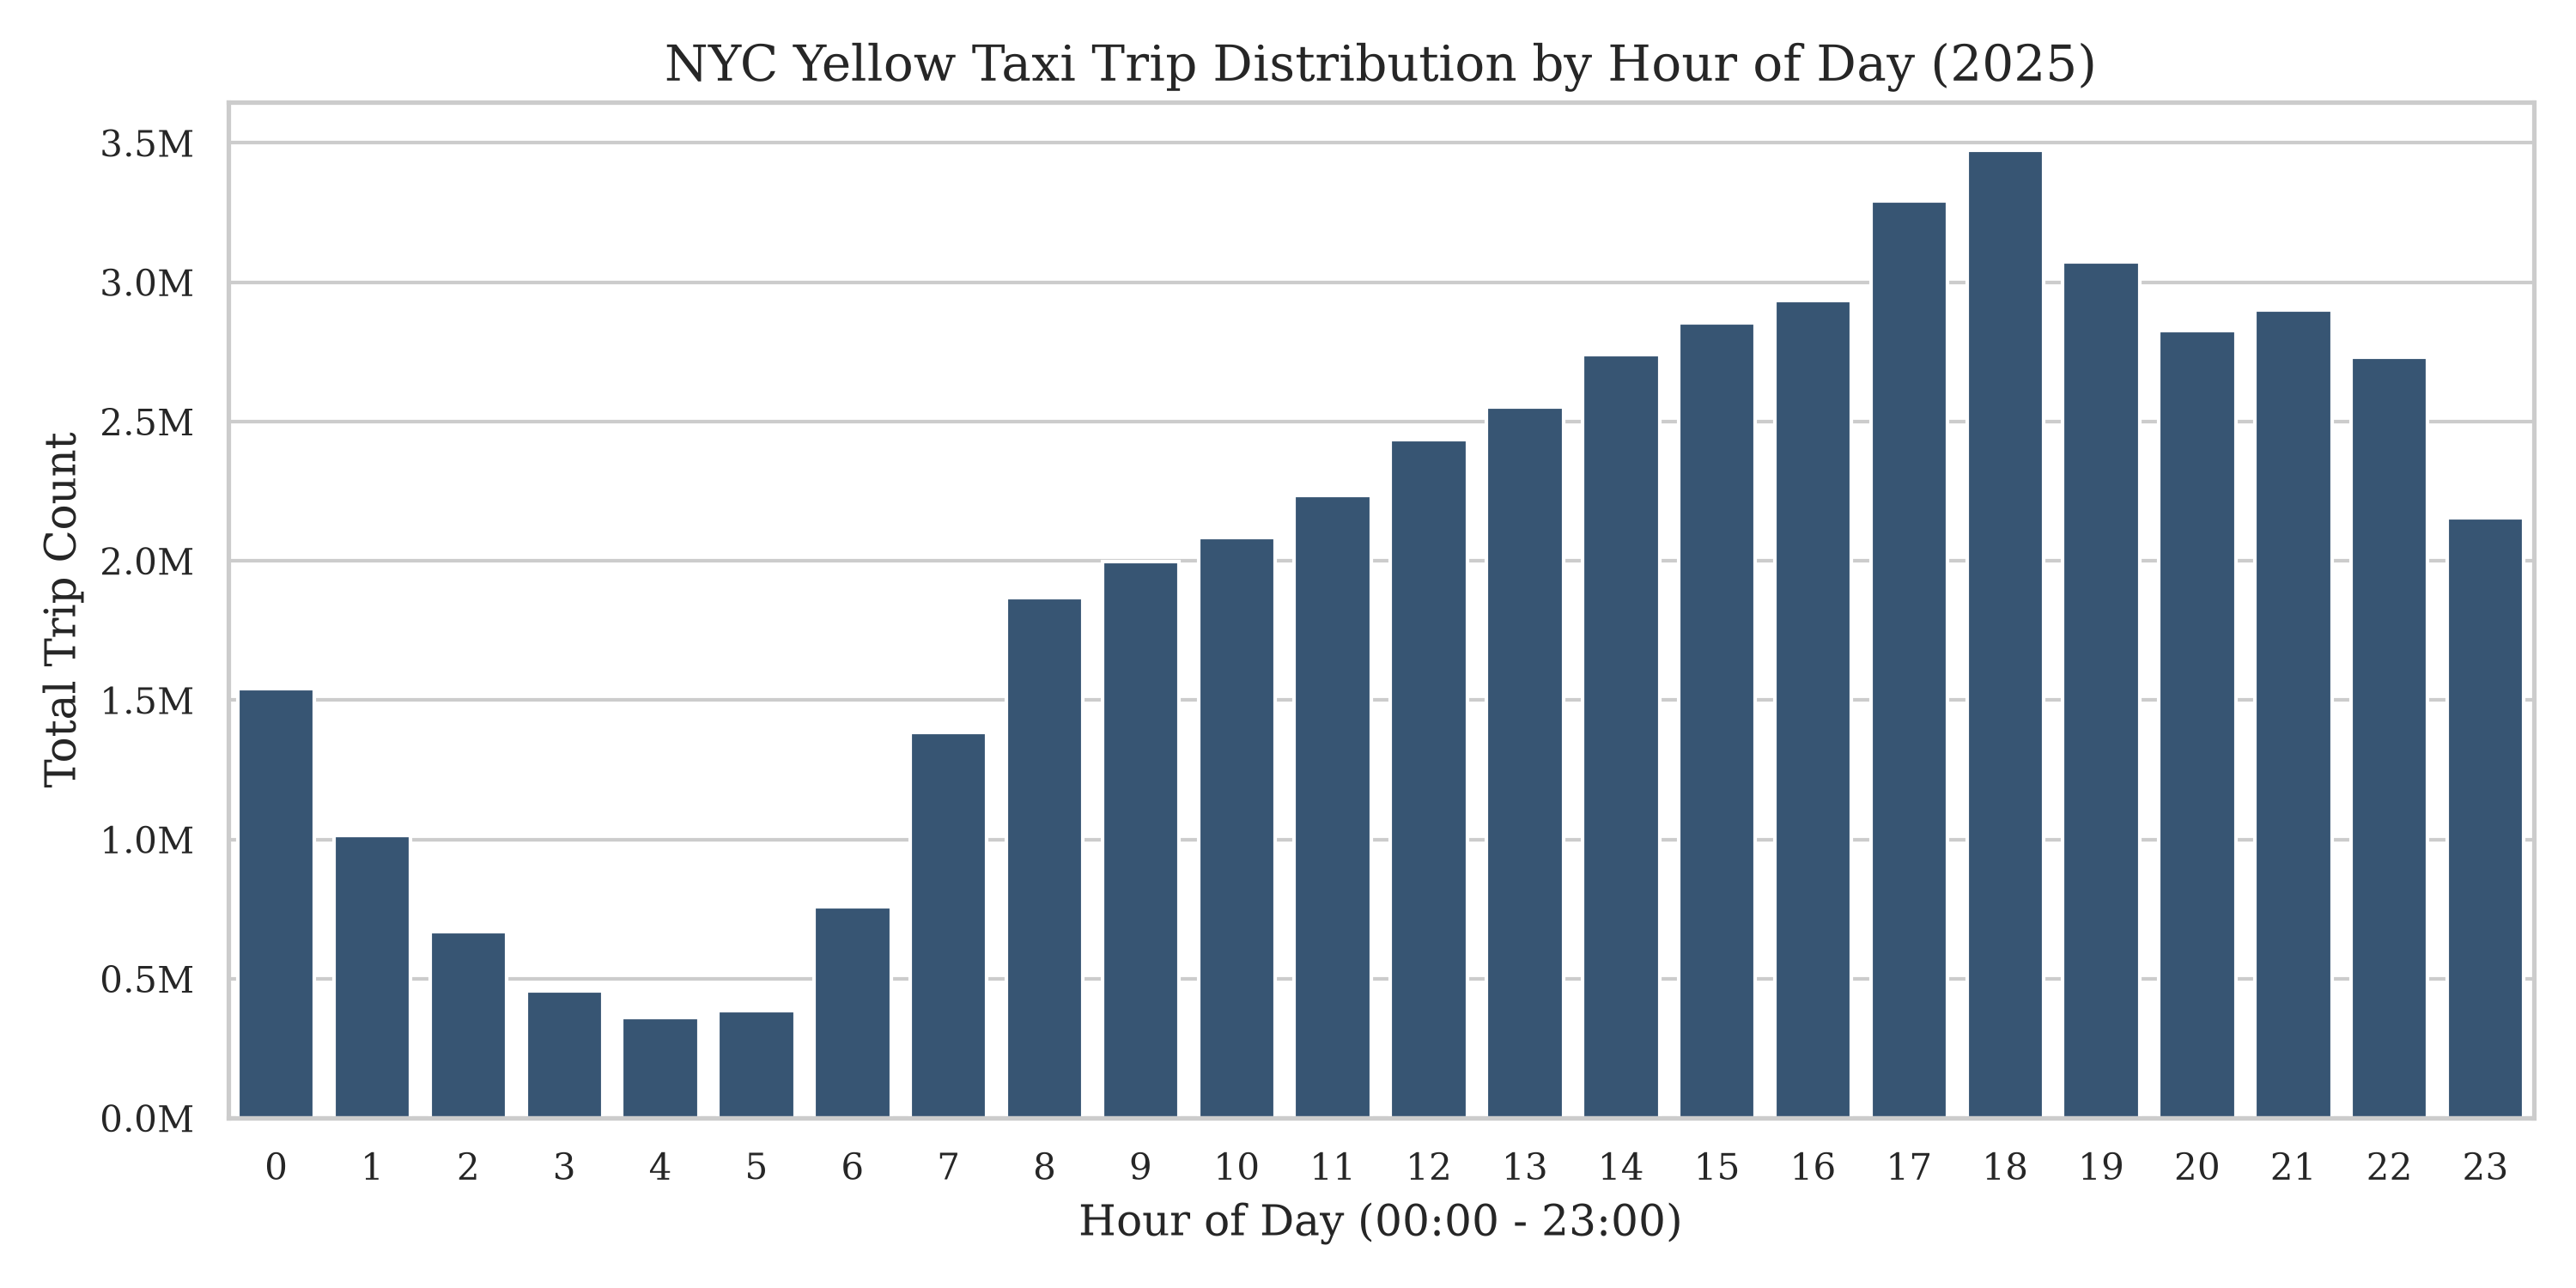
\includegraphics[width=\textwidth]{../figures/hourly_distribution.png}
        \caption{Hourly Trip Distribution}
        \label{fig:hourly}
    \end{subfigure}
    \hfill
    \begin{subfigure}[b]{0.48\textwidth}
        \centering
        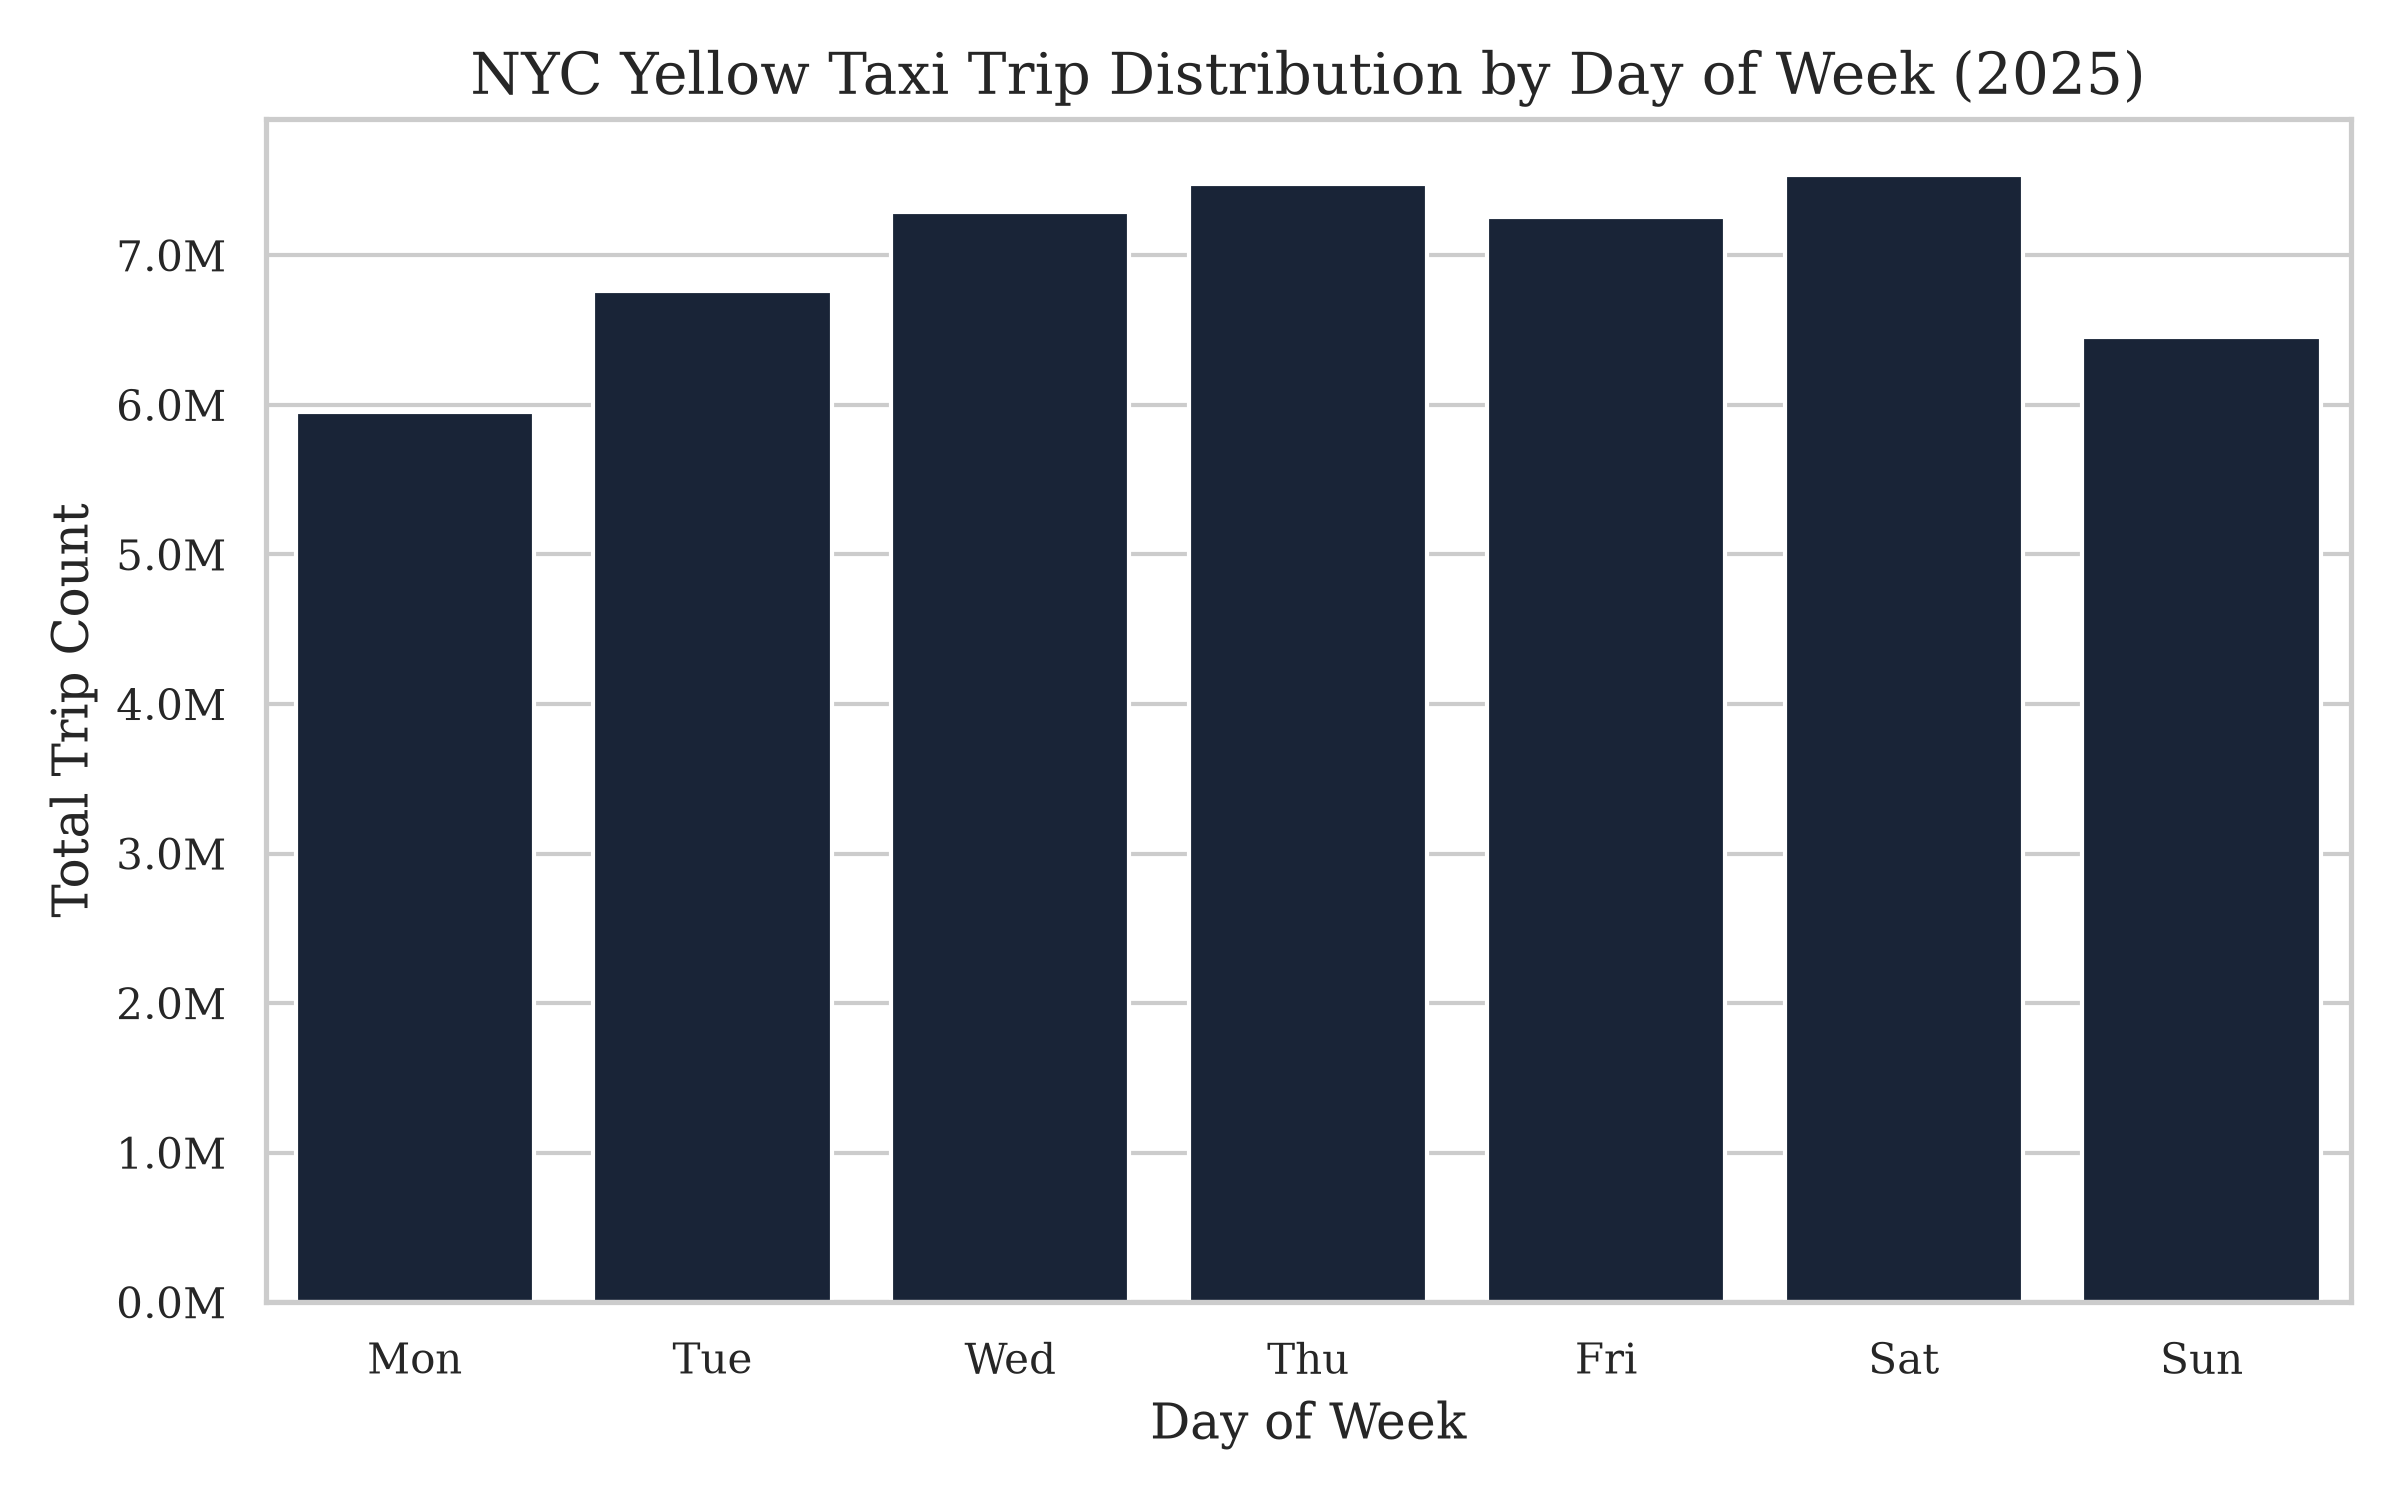
\includegraphics[width=\textwidth]{../figures/dow_distribution.png}
        \caption{Day of Week Distribution}
        \label{fig:dow}
    \end{subfigure}
    
    \vspace{1em} % Vertical spacing between rows
    
    % Second Row
    \begin{subfigure}[b]{0.48\textwidth}
        \centering
        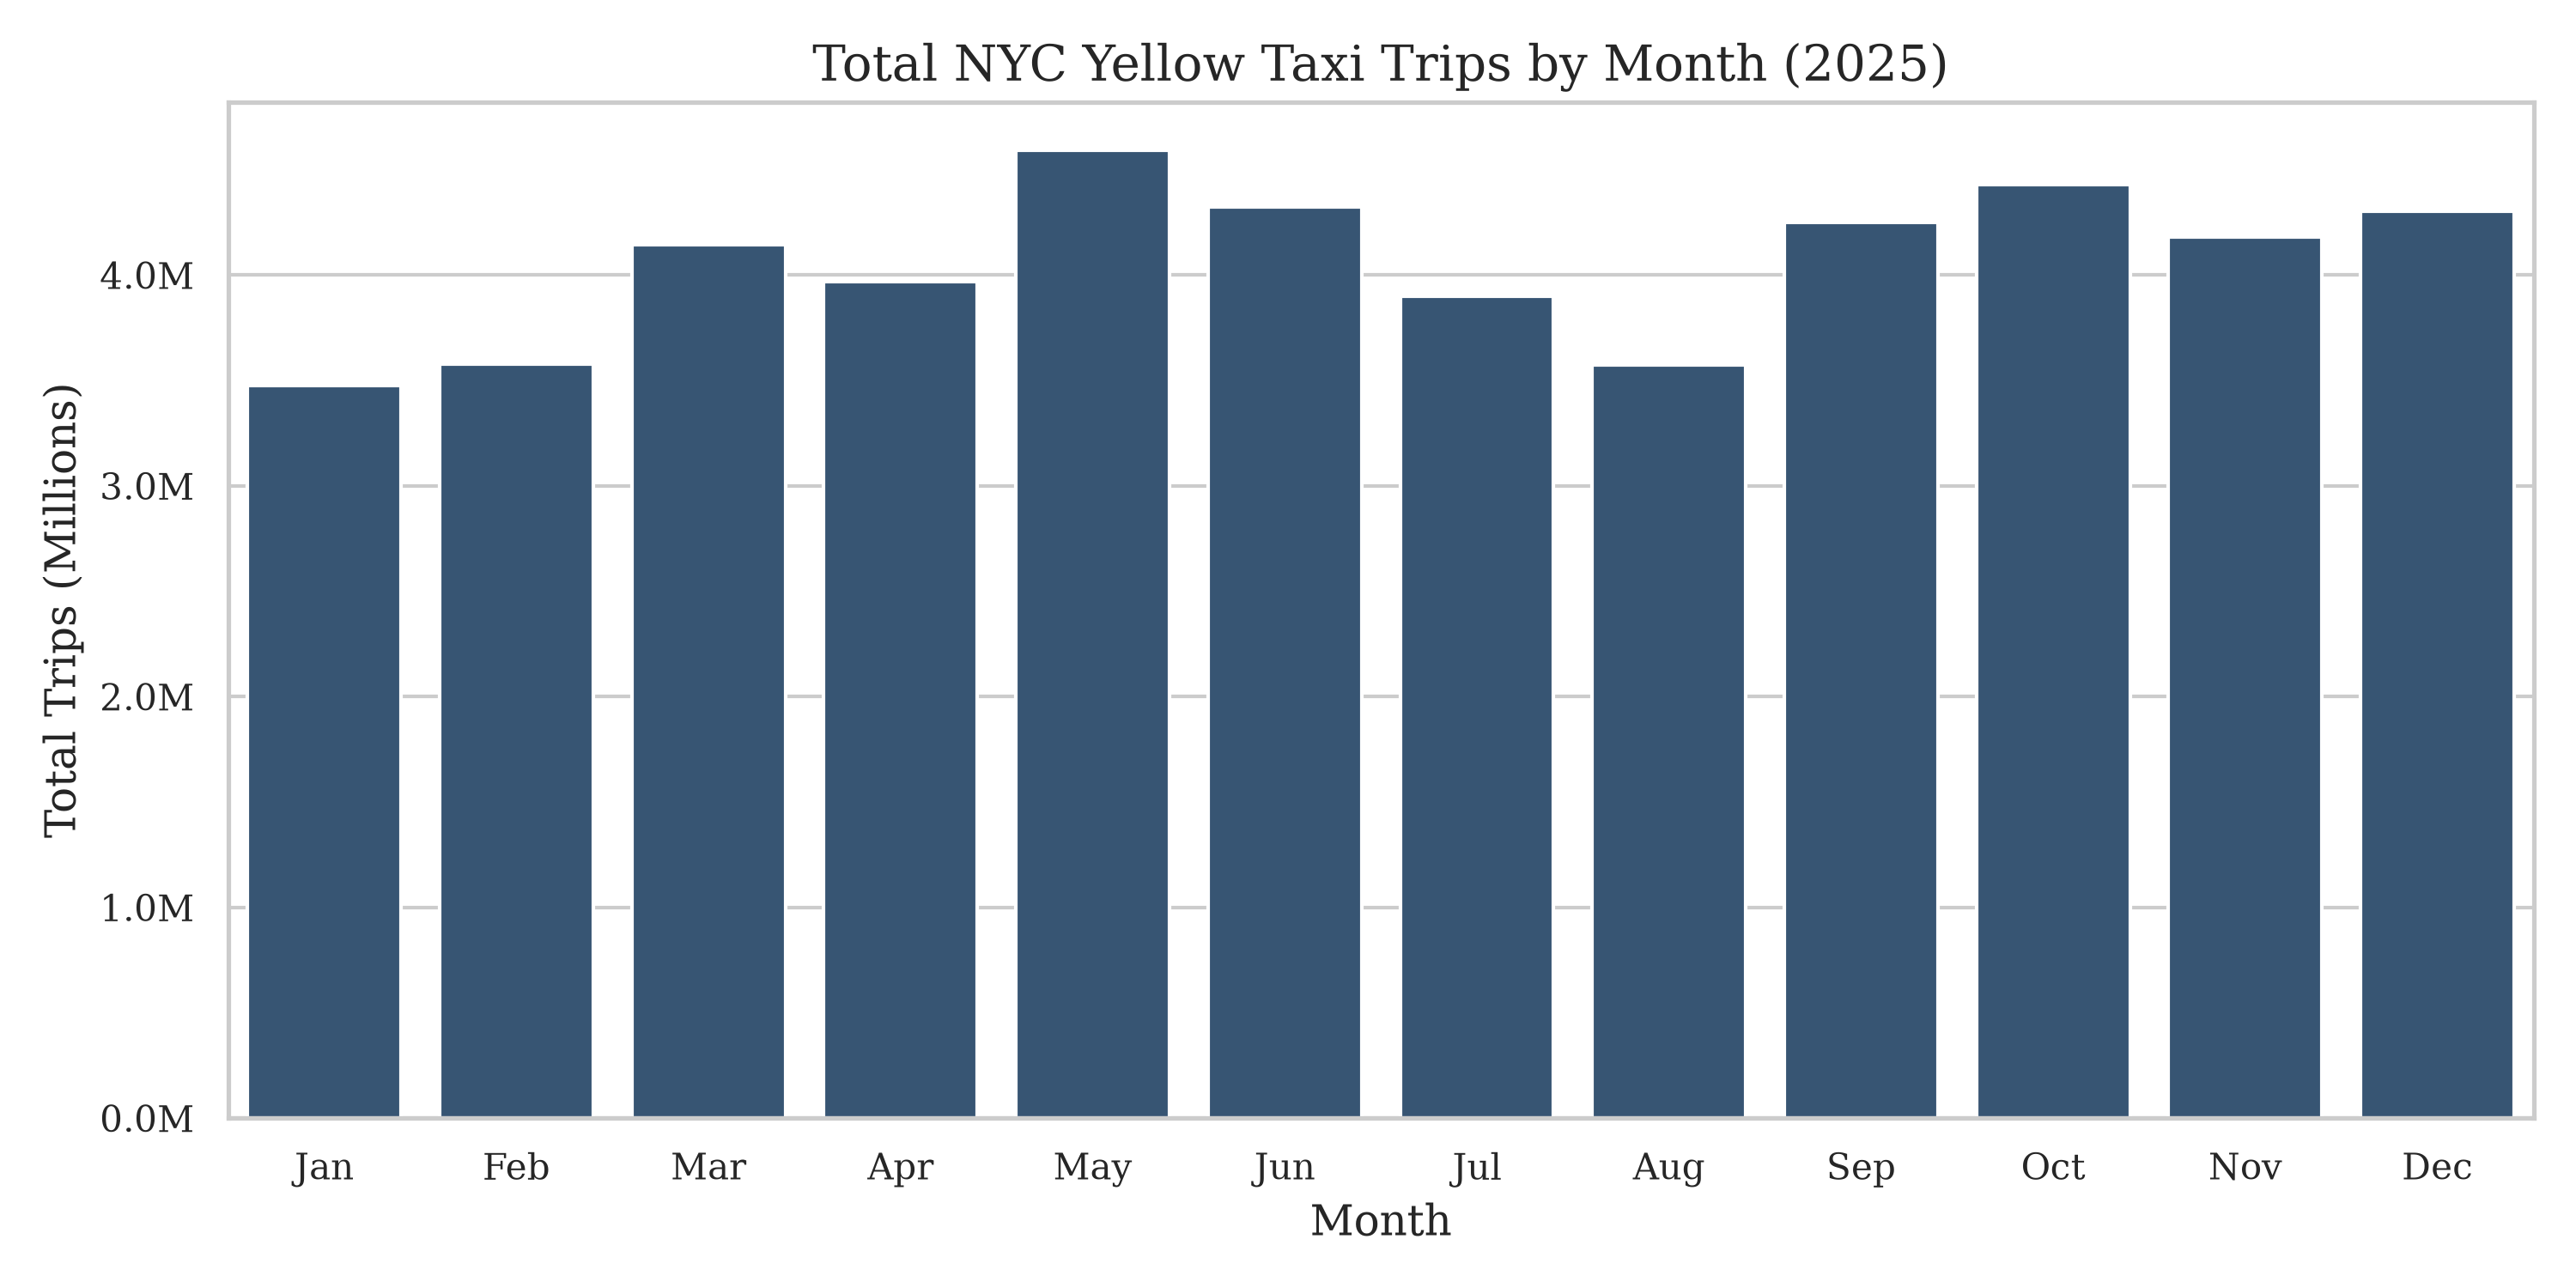
\includegraphics[width=\textwidth]{../figures/monthly_distribution.png}
        \caption{Monthly Trip Volume}
        \label{fig:monthly}
    \end{subfigure}
    \hfill
    \begin{subfigure}[b]{0.48\textwidth}
        \centering
        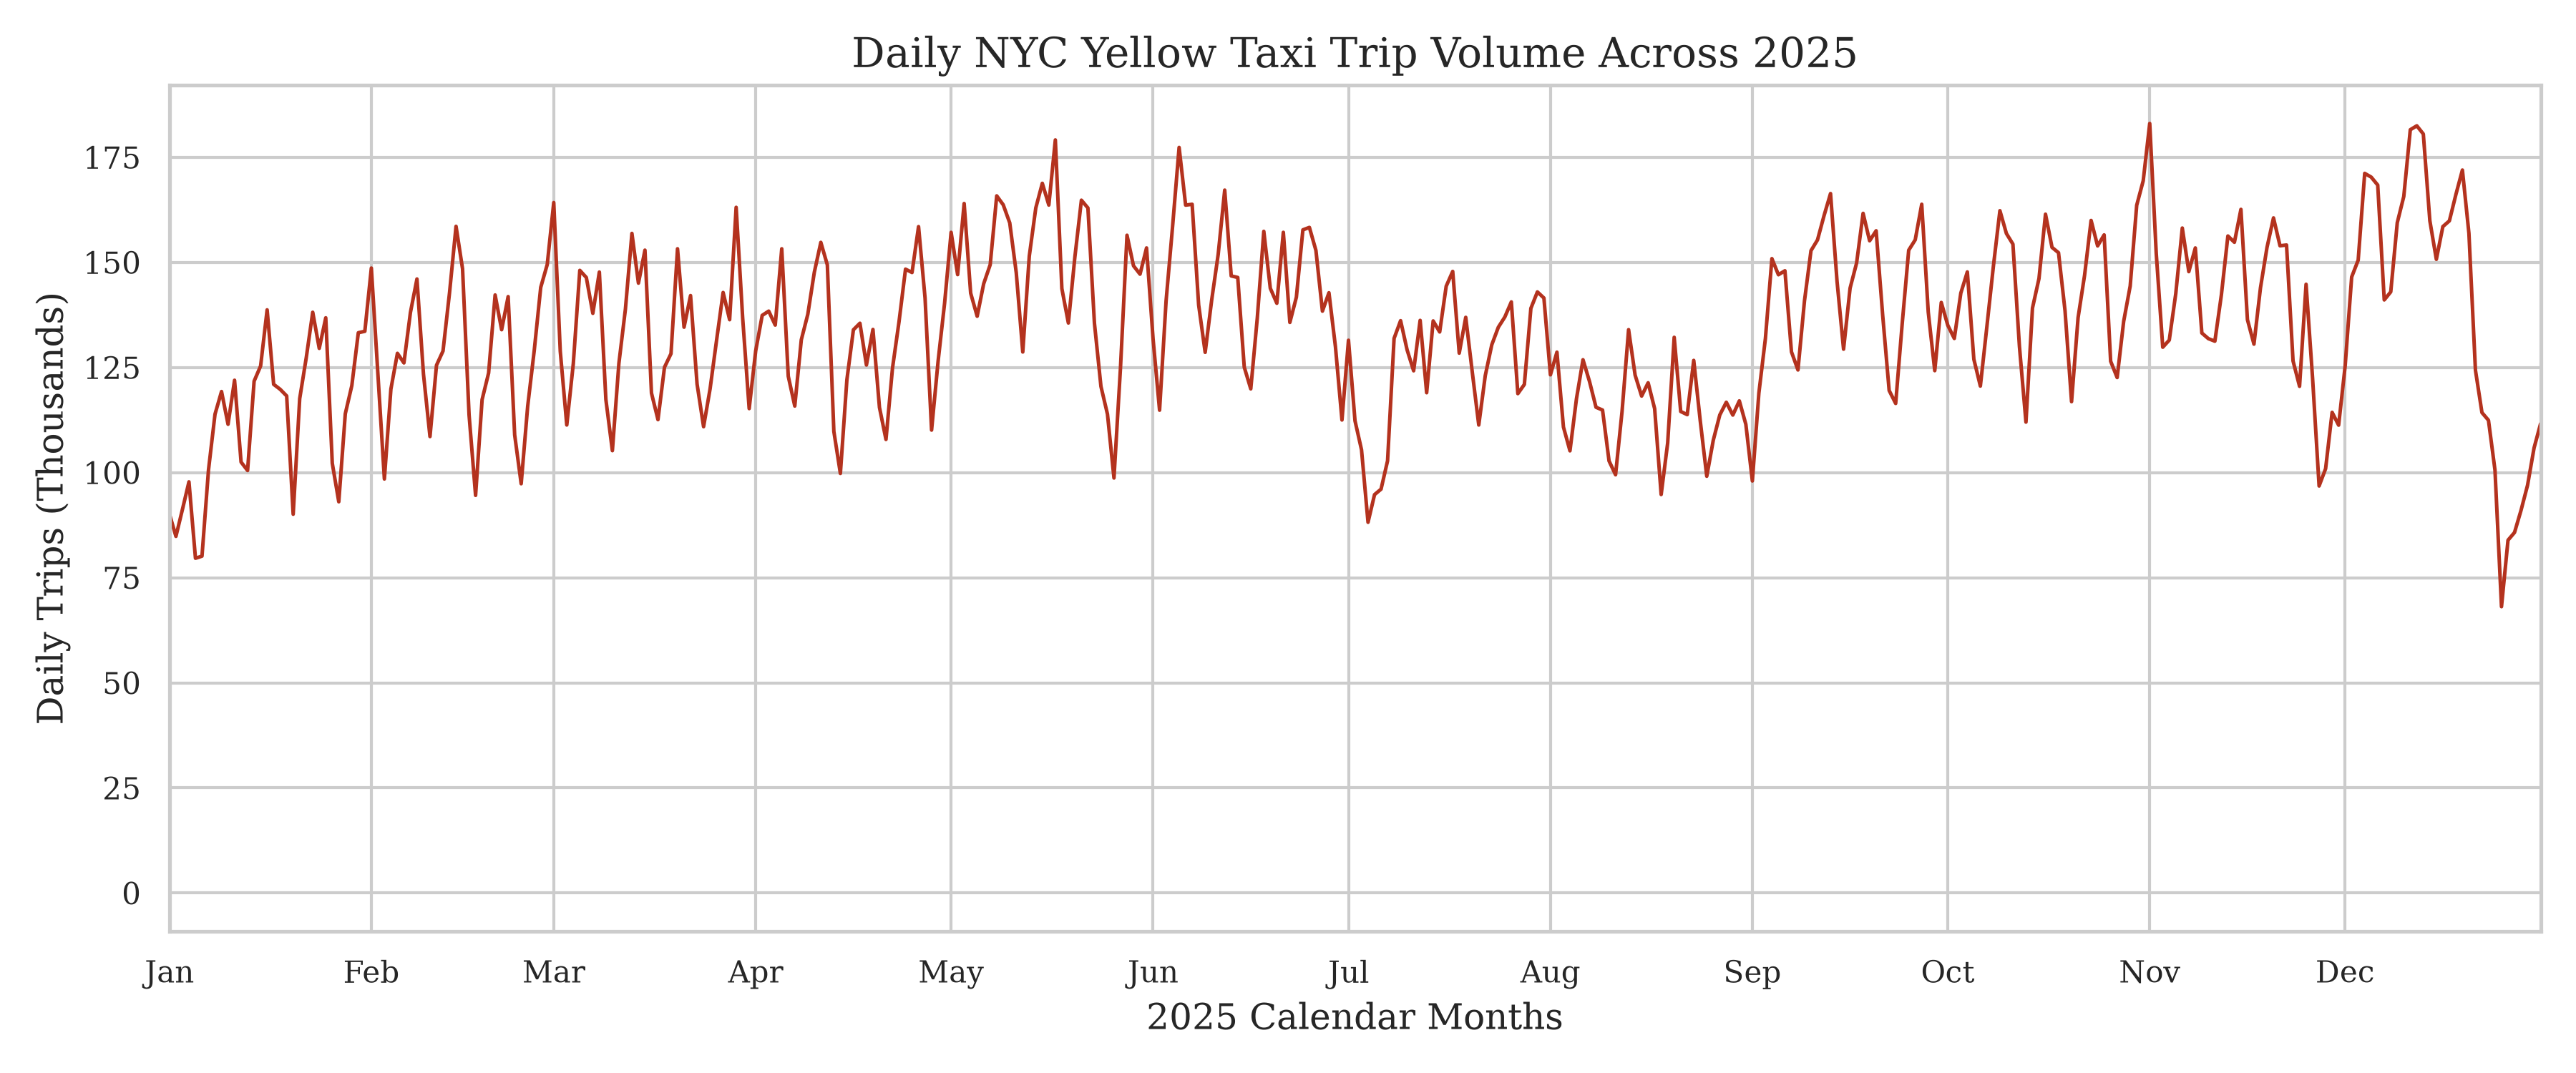
\includegraphics[width=\textwidth]{../figures/daily_timeseries.png}
        \caption{Daily Time Series}
        \label{fig:daily}
    \end{subfigure}
    
    \caption{Temporal Distribution and Time Series Analysis of NYC Yellow Taxi Trips (2025)}
    \label{fig:temporal_grid}
\end{figure}

\begin{itemize}
    \item \textbf{Intra-Day Hourly Patterns:}
     Trip volumes follow a distinct bimodal commuter curve (Figure~\ref{fig:hourly}). Activity hits its nightly trough between 03:00 and 05:00 AM ($\approx 0.35\text{M}$ trips), ramps up steadily through the morning, and peaks sharply during the evening rush hour at 18:00 (6:00 PM) with nearly $3.5\text{M}$ annual originations.
    \item 
    \textbf{Inter-Day Weekly Patterns:} 

    Weekly activity (Figure~\ref{fig:dow}) remains robust from Tuesday through Saturday, with Saturday recording the highest aggregate volume ($\approx 7.5\text{M}$ trips), driven by weekend entertainment and nightlife mobility. Monday experiences a relative weekly lull ($\approx 5.9\text{M}$ trips).
    
    \item \textbf{Monthly \& Longitudinal Trends:} 
    Monthly aggregation (Figure~\ref{fig:monthly}) highlights peak seasonal volume in May ($\approx 4.6\text{M}$ trips), while the daily time-series trend across all 365 calendar days of 2025 (Figure~\ref{fig:daily}) confirms complete temporal data continuity with zero missing daily partitions and consistent weekly oscillations.
\end{itemize}



\subsection{Exploratory Data Analysis: Trip Distance}
\label{sec:eda_trip_distance}

The \texttt{trip\_distance} variable records the total elapsed distance of a journey in miles as measured by the taximeter. Analyzing the distribution of trip distance before and after cleaning provides critical insight into how physical anomalies distort summary metrics and demonstrates the efficacy of our preprocessing protocols.

\begin{table}[htbp]
\centering
\caption{Pre- and Post-Cleansing Descriptive Statistics for Trip Distance (2025 Dataset)}
\label{tab:stats_trip_distance_comparison}
\small
\begin{tabular}{lrr}
\toprule
\textbf{Metric} & \textbf{Pre-Cleansing (Raw)} & \textbf{Post-Cleansing (Clean)} \\
\midrule
Total Records ($N$) & 48,722,602 & 44,015,208 \\
Mean ($\mu$) & 6.84 miles & 3.49 miles \\
25th Percentile ($Q_1$) & 1.04 miles & 1.10 miles \\
Median ($Q_2$) & 1.85 miles & 1.89 miles \\
75th Percentile ($Q_3$) & 3.70 miles & 3.73 miles \\
Standard Deviation ($\sigma$) & 649.36 miles & 4.32 miles \\
Interquartile Range (IQR) & 2.66 miles & 2.63 miles \\
Skewness & 240.90 & 3.09 \\
\bottomrule
\end{tabular}
\end{table}

\subsubsection{Statistical Characteristics and Cleansing Impact Analysis}
As detailed in Table~\ref{tab:stats_trip_distance_comparison}, the raw dataset exhibits extreme sensitivity to telemetry noise and recording corruptions:
\begin{itemize}
    \item \textbf{Impact on Dispersion and Variance:} In the pre-cleansing dataset, the standard deviation ($\sigma = 649.36$ miles) was nearly $100\times$ larger than the mean, driven by extreme GPS satellite jump errors logging distances in excess of $4,000$ miles for sub-hour trips. Following our cleaning pipeline, the standard deviation stabilizes at $4.32$ miles, accurately capturing natural variability across local street hails and regional trips.
    \item \textbf{Impact on Skewness:} Raw telemetry errors introduced an immense positive skewness of $240.90$. Removing non-physical artifacts reduced skewness by over $98\%$ down to a natural right-skewed value of $3.09$.
    \item \textbf{Stability of Robust Non-Parametric Measures:} While the mean dropped sharply from $6.84$ miles to $3.49$ miles (due to the removal of multi-thousand-mile GPS glitches and zero-distance stationary records), robust order statistics remained remarkably stable. The median shifted slightly from $1.85$ to $1.89$ miles, and the IQR moved from $2.66$ to $2.63$ miles, proving that our cleansing protocol removes gross artifacts without corrupting the core underlying trip distribution.
\end{itemize}

The probability density function (Figure~\ref{fig:trip_distance_dist}) shows a dense concentration of mass below $3$ miles, representing routine intra-Manhattan journeys, followed by an extended positive tail for airport and regional transfers.

\begin{figure}[htbp]
    \centering
    \begin{subfigure}[b]{0.48\textwidth}
        \centering
        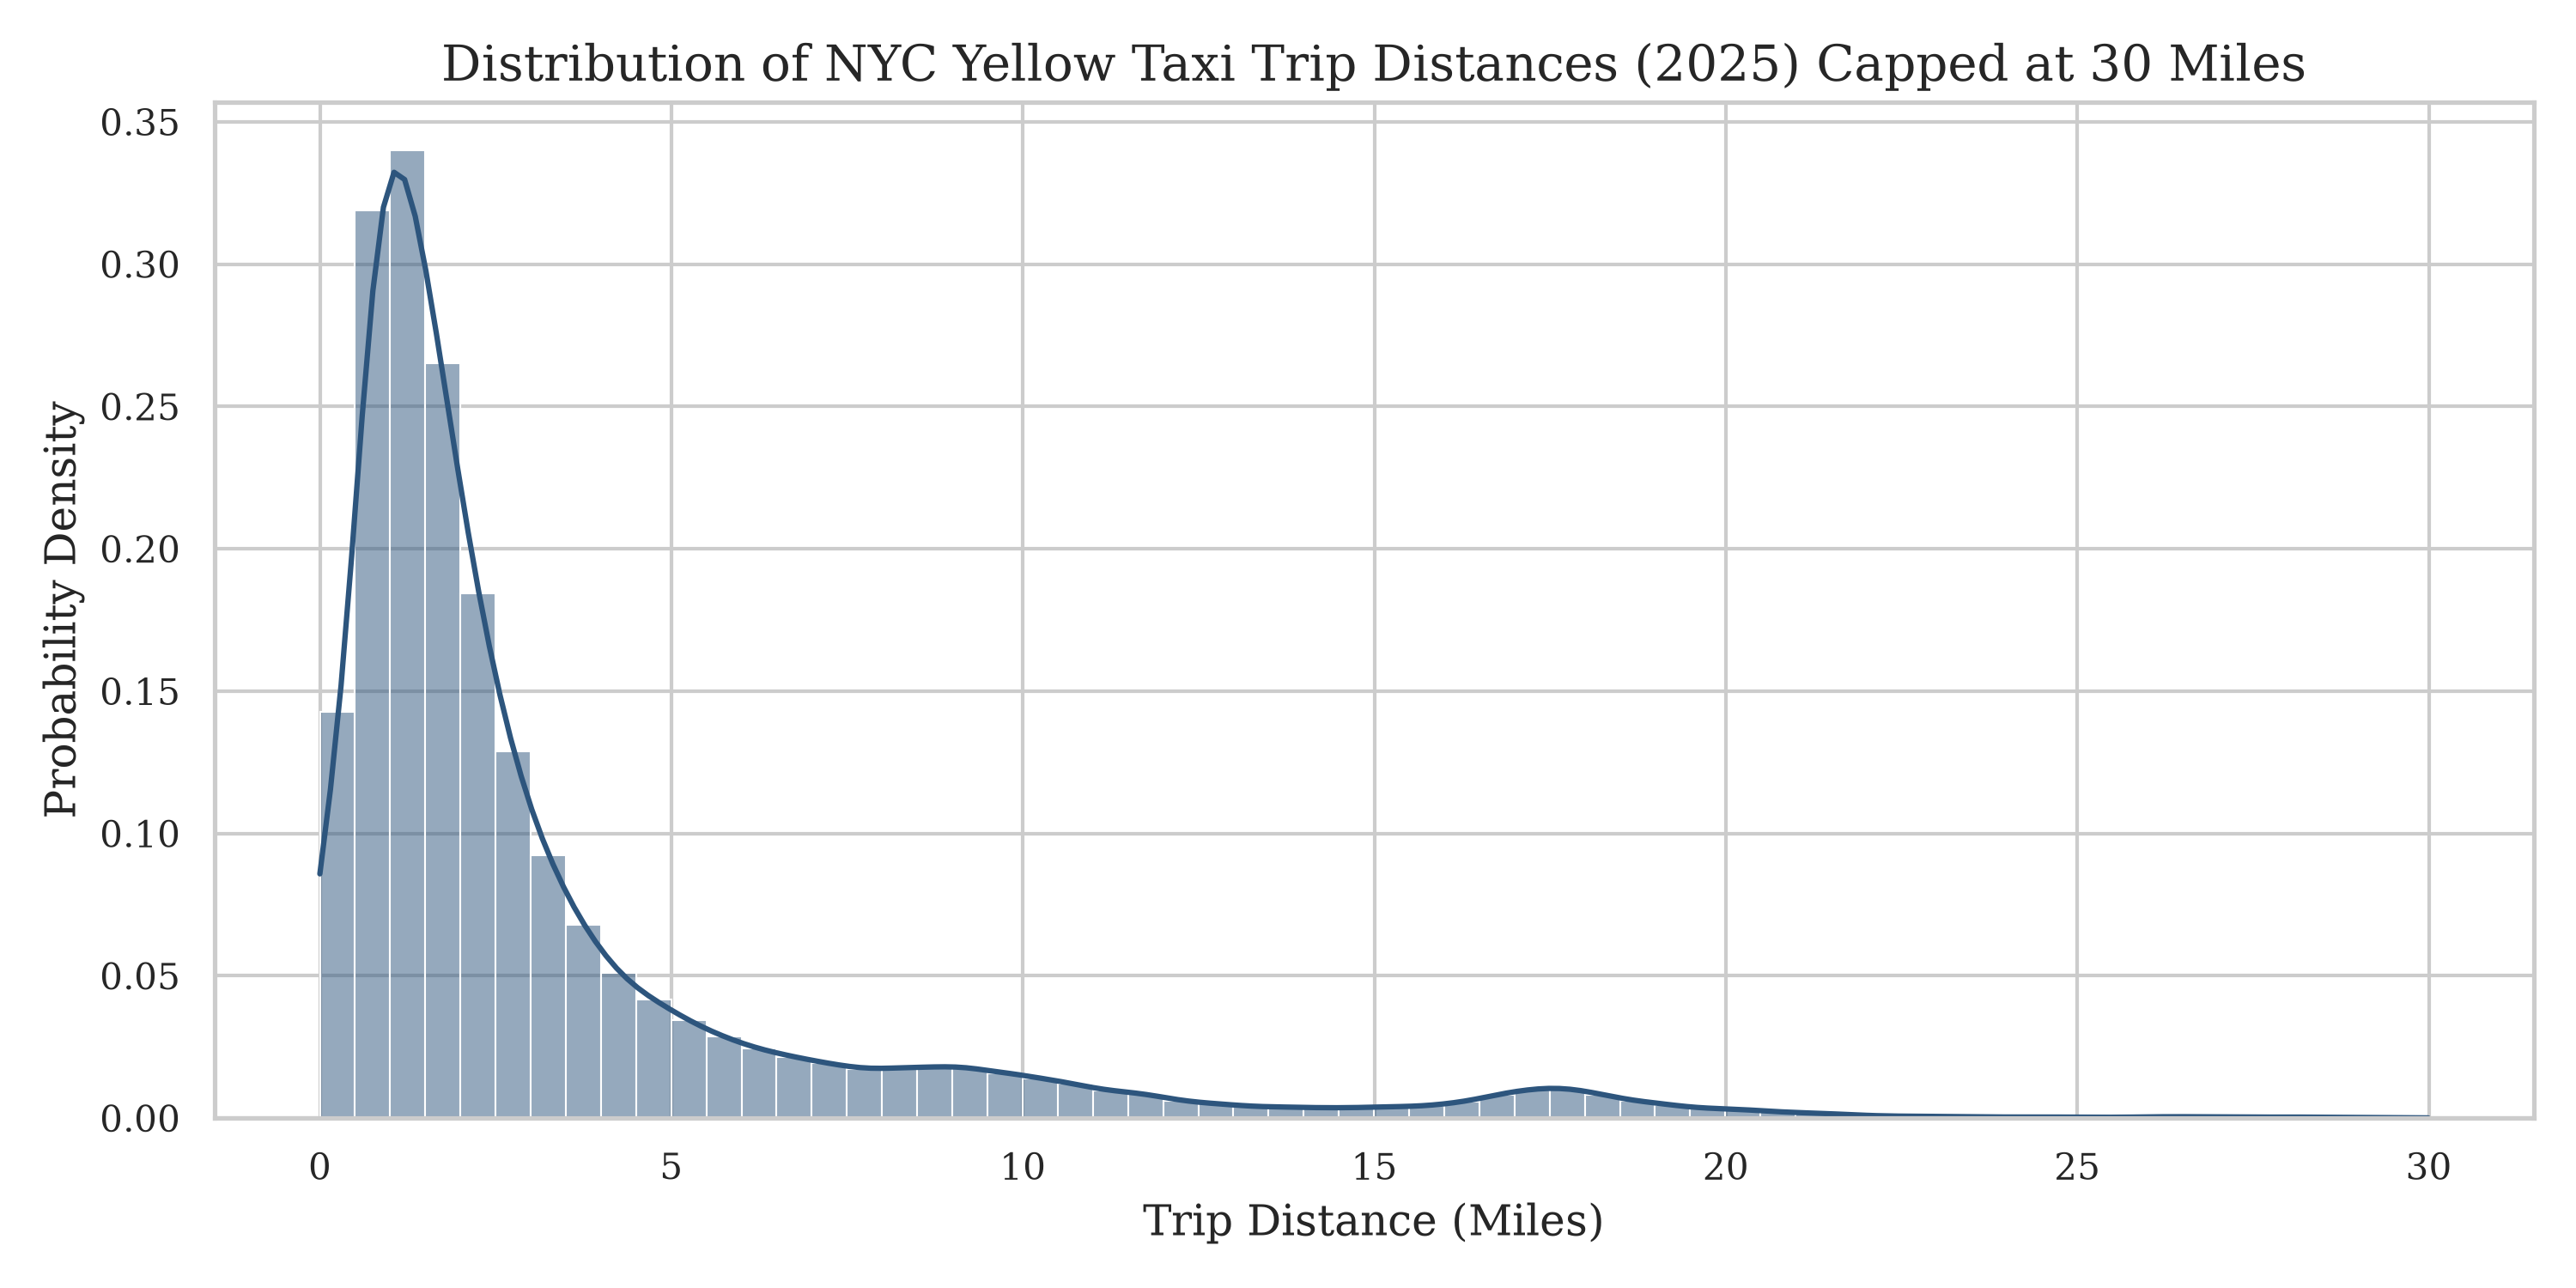
\includegraphics[width=\textwidth]{../figures/trip_distance_distribution.png}
        \caption{Probability Density Distribution Capped at 30 Miles}
        \label{fig:trip_distance_dist}
    \end{subfigure}
    \hfill
    \begin{subfigure}[b]{0.48\textwidth}
        \centering
        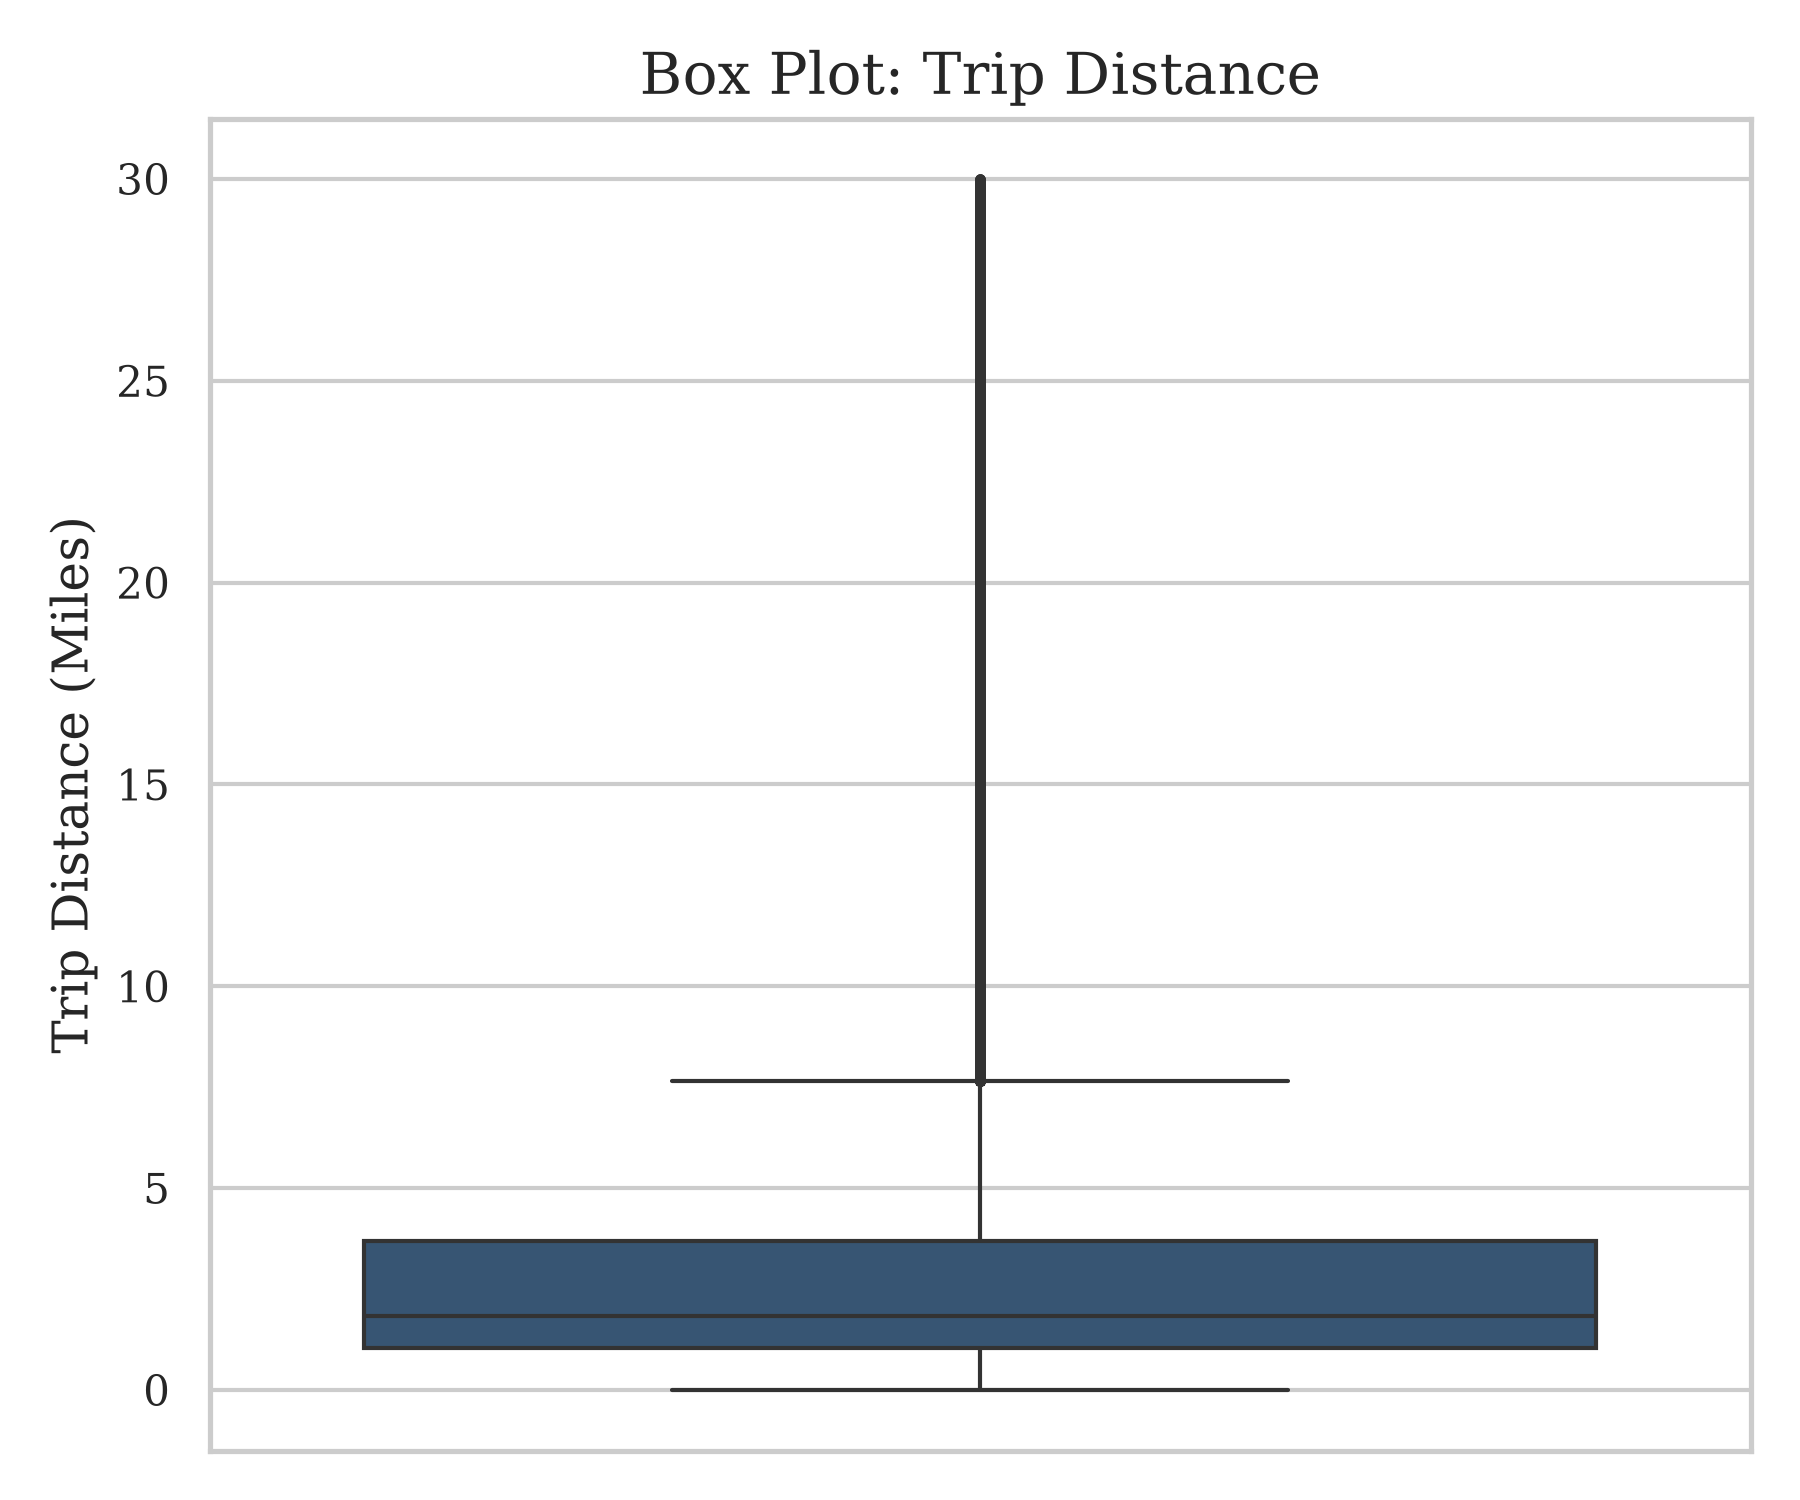
\includegraphics[width=\textwidth]{../figures/trip_distance_boxplot.png}
        \caption{Box Plot (Capped at 30 Miles)}
        \label{fig:trip_distance_box}
    \end{subfigure}
    \caption{Distribution and Box Plot Analysis for Filtered Trip Distance (2025)}
    \label{fig:trip_distance_analysis}
\end{figure}

\subsubsection{Long-Distance Trips and Outlier Analysis ($>30$ Miles)}
A detailed query of clean trips exceeding $30$ miles yields a total of \textbf{40,395 valid long-distance trips} across the 2025 dataset ($\approx 0.092\%$ of the pristine baseline population). Table~\ref{tab:long_distance_trips} lists a representative sample of these extreme-distance records ordered by descending distance.

\begin{table}[htbp]
\centering
\caption{Sample of Long-Distance Yellow Taxi Trips Exceeding 30 Miles (2025)}
\label{tab:long_distance_trips}
\tiny
\begin{tabularx}{\textwidth}{llrrlrrlXX}
\toprule
\textbf{Pickup Time} & \textbf{Dropoff Time} & \textbf{Dur (min)} & \textbf{Dist (mi)} & \textbf{Fare (\$)} & \textbf{Speed (mph)} & \textbf{Pass.} & \textbf{Pickup Zone} & \textbf{Dropoff Zone} \\
\midrule
2025-08-30 19:16 & 2025-08-30 22:24 & 188.35 & 197.54 & \$450.00 & 62.93 & 1 & Flushing Meadows-Corona Park & Outside of NYC \\
2025-05-22 01:43 & 2025-05-22 05:23 & 220.20 & 197.27 & \$550.00 & 53.75 & 1 & JFK Airport & Outside of NYC \\
2025-03-13 21:33 & 2025-03-14 00:51 & 197.85 & 195.72 & \$450.00 & 59.35 & 1 & JFK Airport & Outside of NYC \\
2025-12-31 16:32 & 2025-12-31 20:05 & 213.77 & 195.33 & \$1295.90 & 54.83 & 2 & JFK Airport & Outside of NYC \\
2025-04-18 15:34 & 2025-04-18 19:08 & 213.95 & 194.85 & \$1303.60 & 54.64 & 1 & JFK Airport & Outside of NYC \\
2025-11-16 11:13 & 2025-11-16 14:49 & 216.82 & 192.97 & \$460.23 & 53.40 & \texttt{NA} & World Trade Center & Outside of NYC \\
2025-06-06 10:00 & 2025-06-06 13:46 & 225.58 & 191.81 & \$800.00 & 51.02 & 3 & East Chelsea & Outside of NYC \\
2025-03-02 06:12 & 2025-03-02 09:32 & 200.53 & 190.50 & \$650.00 & 57.00 & 1 & Springfield Gardens South & Outside of NYC \\
2025-01-21 05:17 & 2025-01-21 08:19 & 181.80 & 188.88 & \$1309.20 & 62.34 & 1 & West Concourse & Outside of NYC \\
2025-01-18 21:07 & 2025-01-19 00:20 & 192.55 & 183.95 & \$503.59 & 57.32 & \texttt{NA} & Clinton East & Outside of NYC \\
\bottomrule
\end{tabularx}
\end{table}

\subsubsection{Justification for Retaining Outliers Beyond the 1.5$\times$IQR Rule}
Applying Tukey's standard fence rule ($Q_3 + 1.5 \times \text{IQR}$) yields an outlier threshold of $3.73 + 1.5 \times (2.63) \approx 7.675$ miles. While standard statistical pipelines might trim records beyond $7.675$ miles, we retain them based on the following justifications:
\begin{enumerate}
    \item \textbf{Legitimate Out-of-Jurisdiction and Regional Transit Activity:} As evidenced in Table~\ref{tab:long_distance_trips}, extreme distance records originate at major transit nodes (JFK, World Trade Center) and terminate at \texttt{Outside of NYC} destinations. These $40,395$ trips represent real, high-value commercial journeys.
    \item \textbf{Economic Integrity and Revenue Preservation:} Removing trips exceeding $7.675$ miles would eliminate a major share of total revenue. Out-of-city journeys command premium fares (up to \$1,309.20 in our sample) and contribute significantly to overall fleet earnings and congestion fees.
    \item \textbf{Prevention of Truncation Bias in Spatial Aggregation:} Trimming valid long-distance journeys would distort origin-destination flow matrices and underestimate regional vehicle turnover times.
    \item \textbf{Methodological Accommodation over Trimming:} Right-skewness ($\text{Skewness} = 3.09$) is accommodated using non-parametric summary measures (median $= 1.89$ miles, $\text{IQR} = 2.63$ miles) and axis capping in visualizations (e.g., $30$ miles in distribution plots) to maintain graphical readability while preserving $100\%$ of authentic economic activity.
\end{enumerate}

\subsection{Exploratory Data Analysis: Fare Amount}
\label{sec:eda_fare_amount}

The \texttt{fare\_amount} variable represents the time-and-distance fare in USD calculated by the taximeter at the conclusion of each trip. Comparing the statistical properties of the fare amount before and after data cleansing illustrates the structural impact of removing negative fare anomalies.

\begin{table}[htbp]
\centering
\caption{Pre- and Post-Cleansing Descriptive Statistics for Fare Amount (2025 Dataset)}
\label{tab:stats_fare_amount_comparison}
\small
\begin{tabular}{lrr}
\toprule
\textbf{Metric} & \textbf{Pre-Cleansing (Raw)} & \textbf{Post-Cleansing (Clean)} \\
\midrule
Total Records ($N$) & 48,722,602 & 44,015,208 \\
Mean ($\mu$) & \$18.42 & \$20.04 \\
25th Percentile ($Q_1$) & \$8.60 & \$9.30 \\
Median ($Q_2$) & \$13.58 & \$14.20 \\
75th Percentile ($Q_3$) & \$22.60 & \$23.30 \\
Standard Deviation ($\sigma$) & \$142.85 & \$149.75 \\
Interquartile Range (IQR) & \$14.00 & \$14.00 \\
Skewness & 5,030.24 & 4,832.47 \\
\bottomrule
\end{tabular}
\end{table}

\subsubsection{Statistical Characteristics and Cleansing Impact Analysis}
As summarized in Table~\ref{tab:stats_fare_amount_comparison}, the median fare increases slightly from $\$13.58$ in the raw dataset to $\$14.20$ after cleaning, while the mean increases from $\$18.42$ to $\$20.04$. 
\begin{itemize}
    \item \textbf{Rationale for Mean Increase:} The upward shift in the mean fare is a direct consequence of filtering out the $2,848,620$ negative fare records (credit card chargebacks, dispute reversals, and administrative adjustments) present in the raw data. Removing these sub-zero financial entries eliminates downward distortion, thereby reflecting the true positive economic value of commercial passenger trips.
    \item \textbf{Distributional Shape:} The distribution continues to exhibit extreme positive skewness ($4,832.47$), driven by a heavy concentration of short, low-cost urban trips combined with an extended right-hand tail of high-value journeys. 
\end{itemize}

The probability density function (Figure~\ref{fig:fare_amount_dist}) reveals a prominent unimodal peak representing standard local city rides ($\$10-\$15$), alongside a distinct structural cluster or secondary bump around $\$70$. This secondary surge corresponds directly to regulated flat-rate airport trips (such as historical or standard JFK airport routes), highlighting a multimodal element embedded within the financial structure of the fleet.

\begin{figure}[htbp]
    \centering
    \begin{subfigure}[b]{0.48\textwidth}
        \centering
        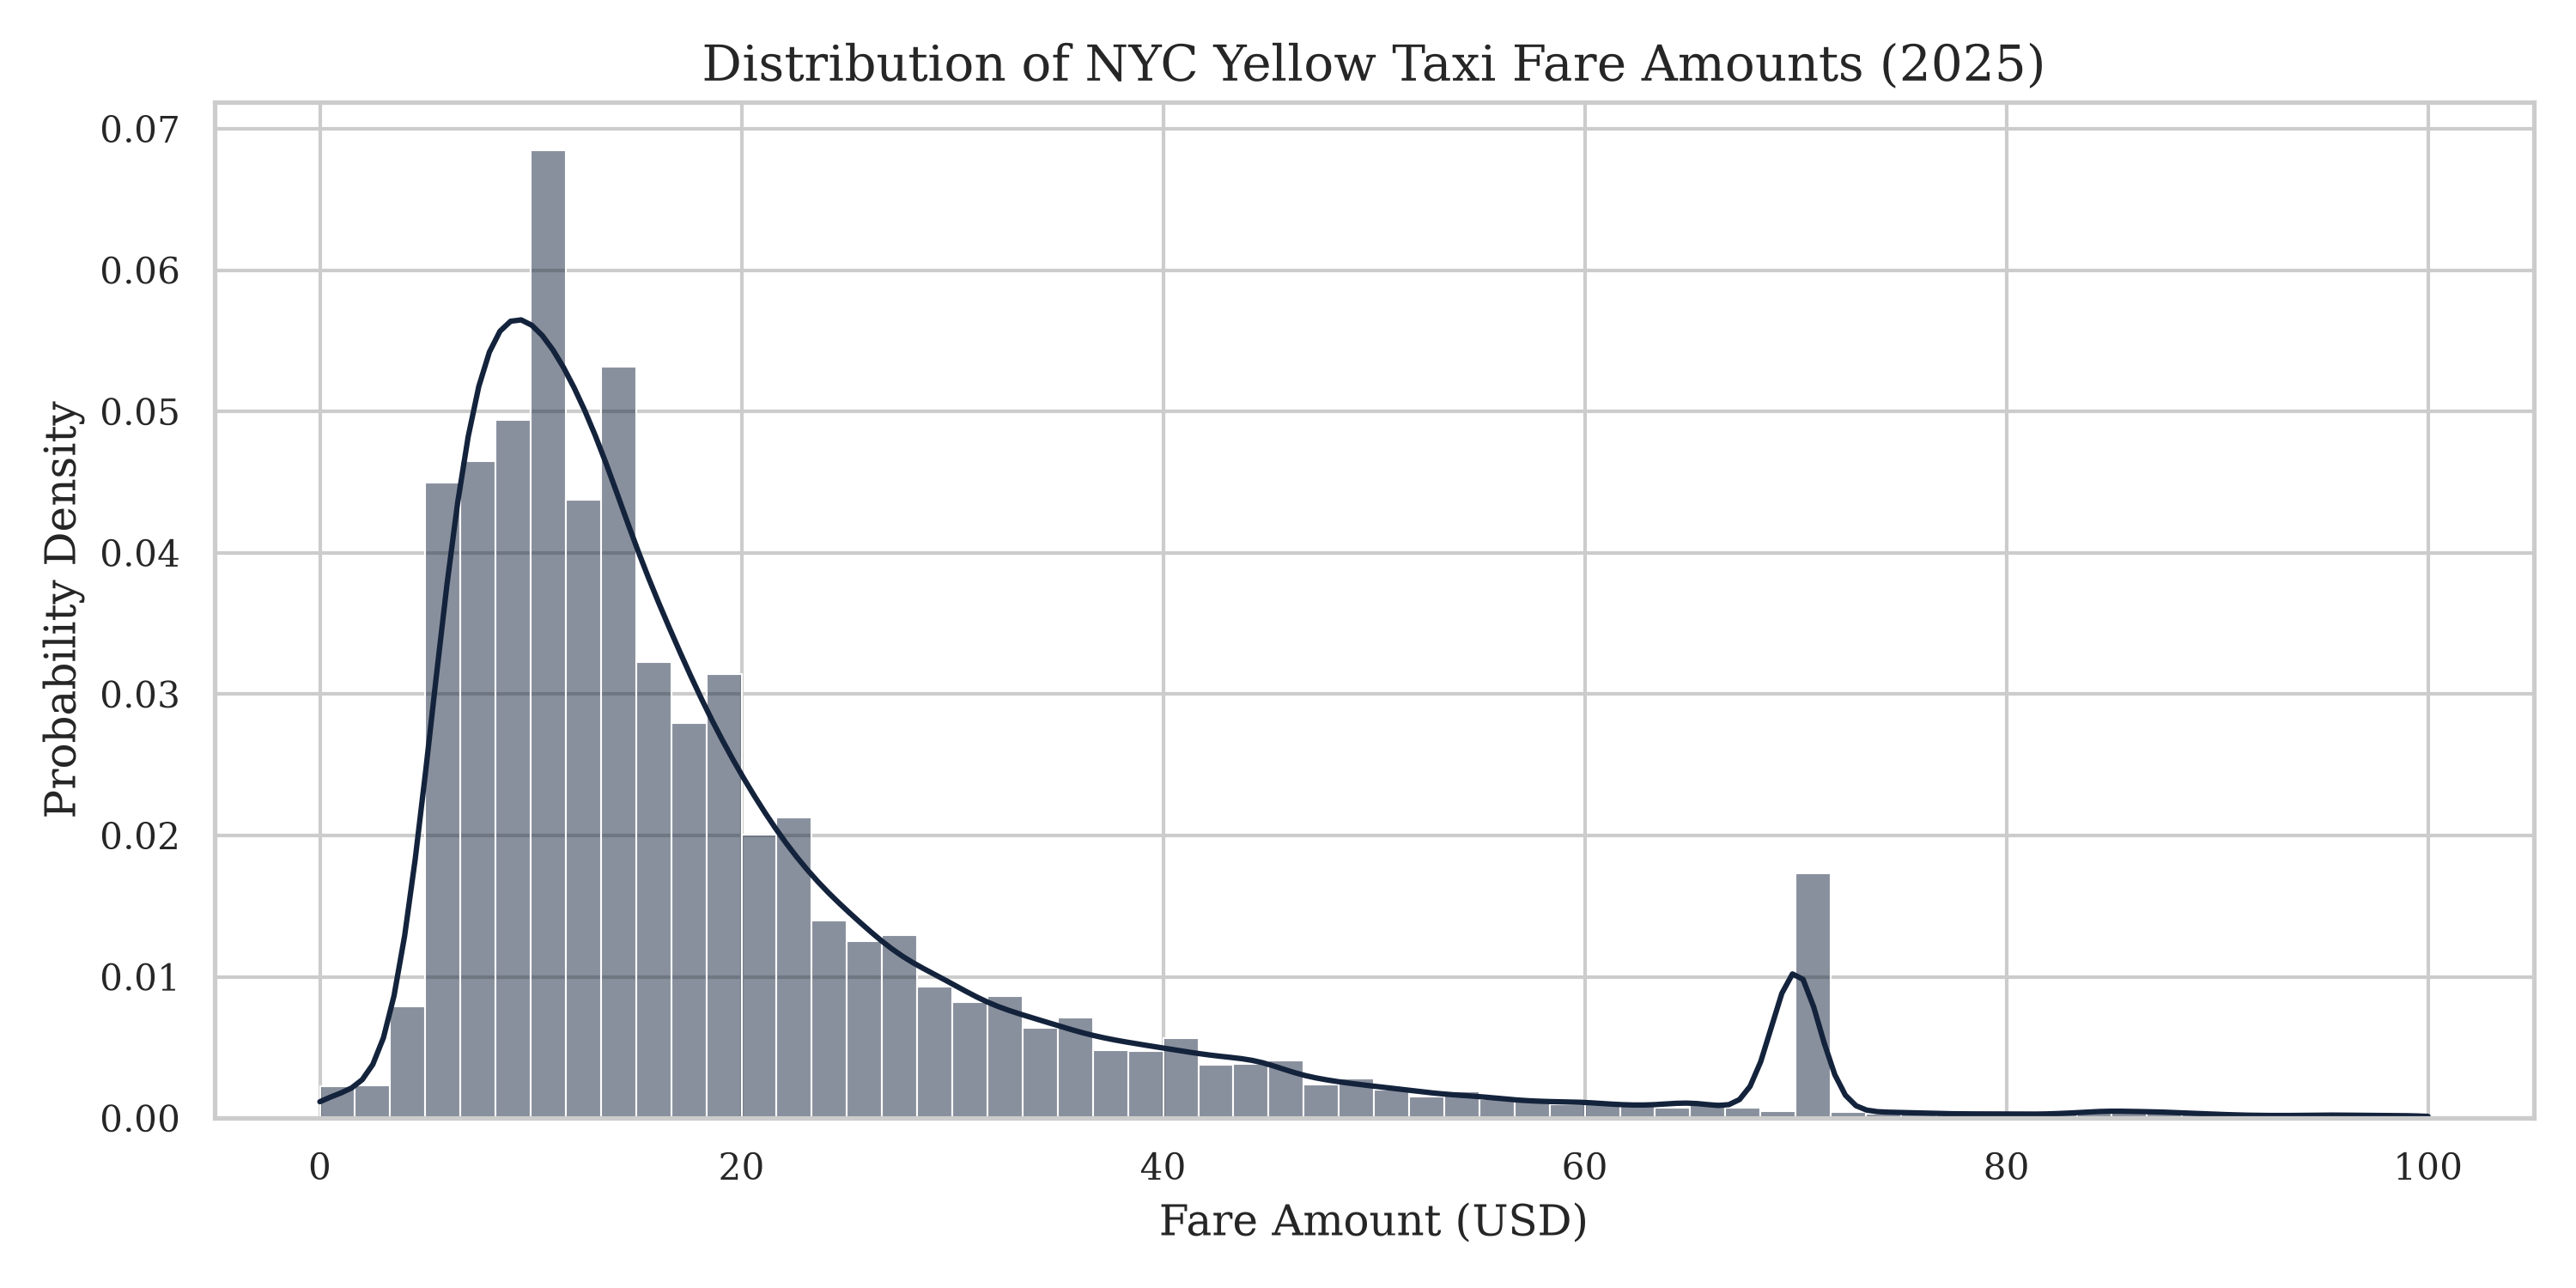
\includegraphics[width=\textwidth]{../figures/fare_amount_distribution.png}
        \caption{Probability Density Distribution}
        \label{fig:fare_amount_dist}
    \end{subfigure}
    \hfill
    \begin{subfigure}[b]{0.48\textwidth}
        \centering
        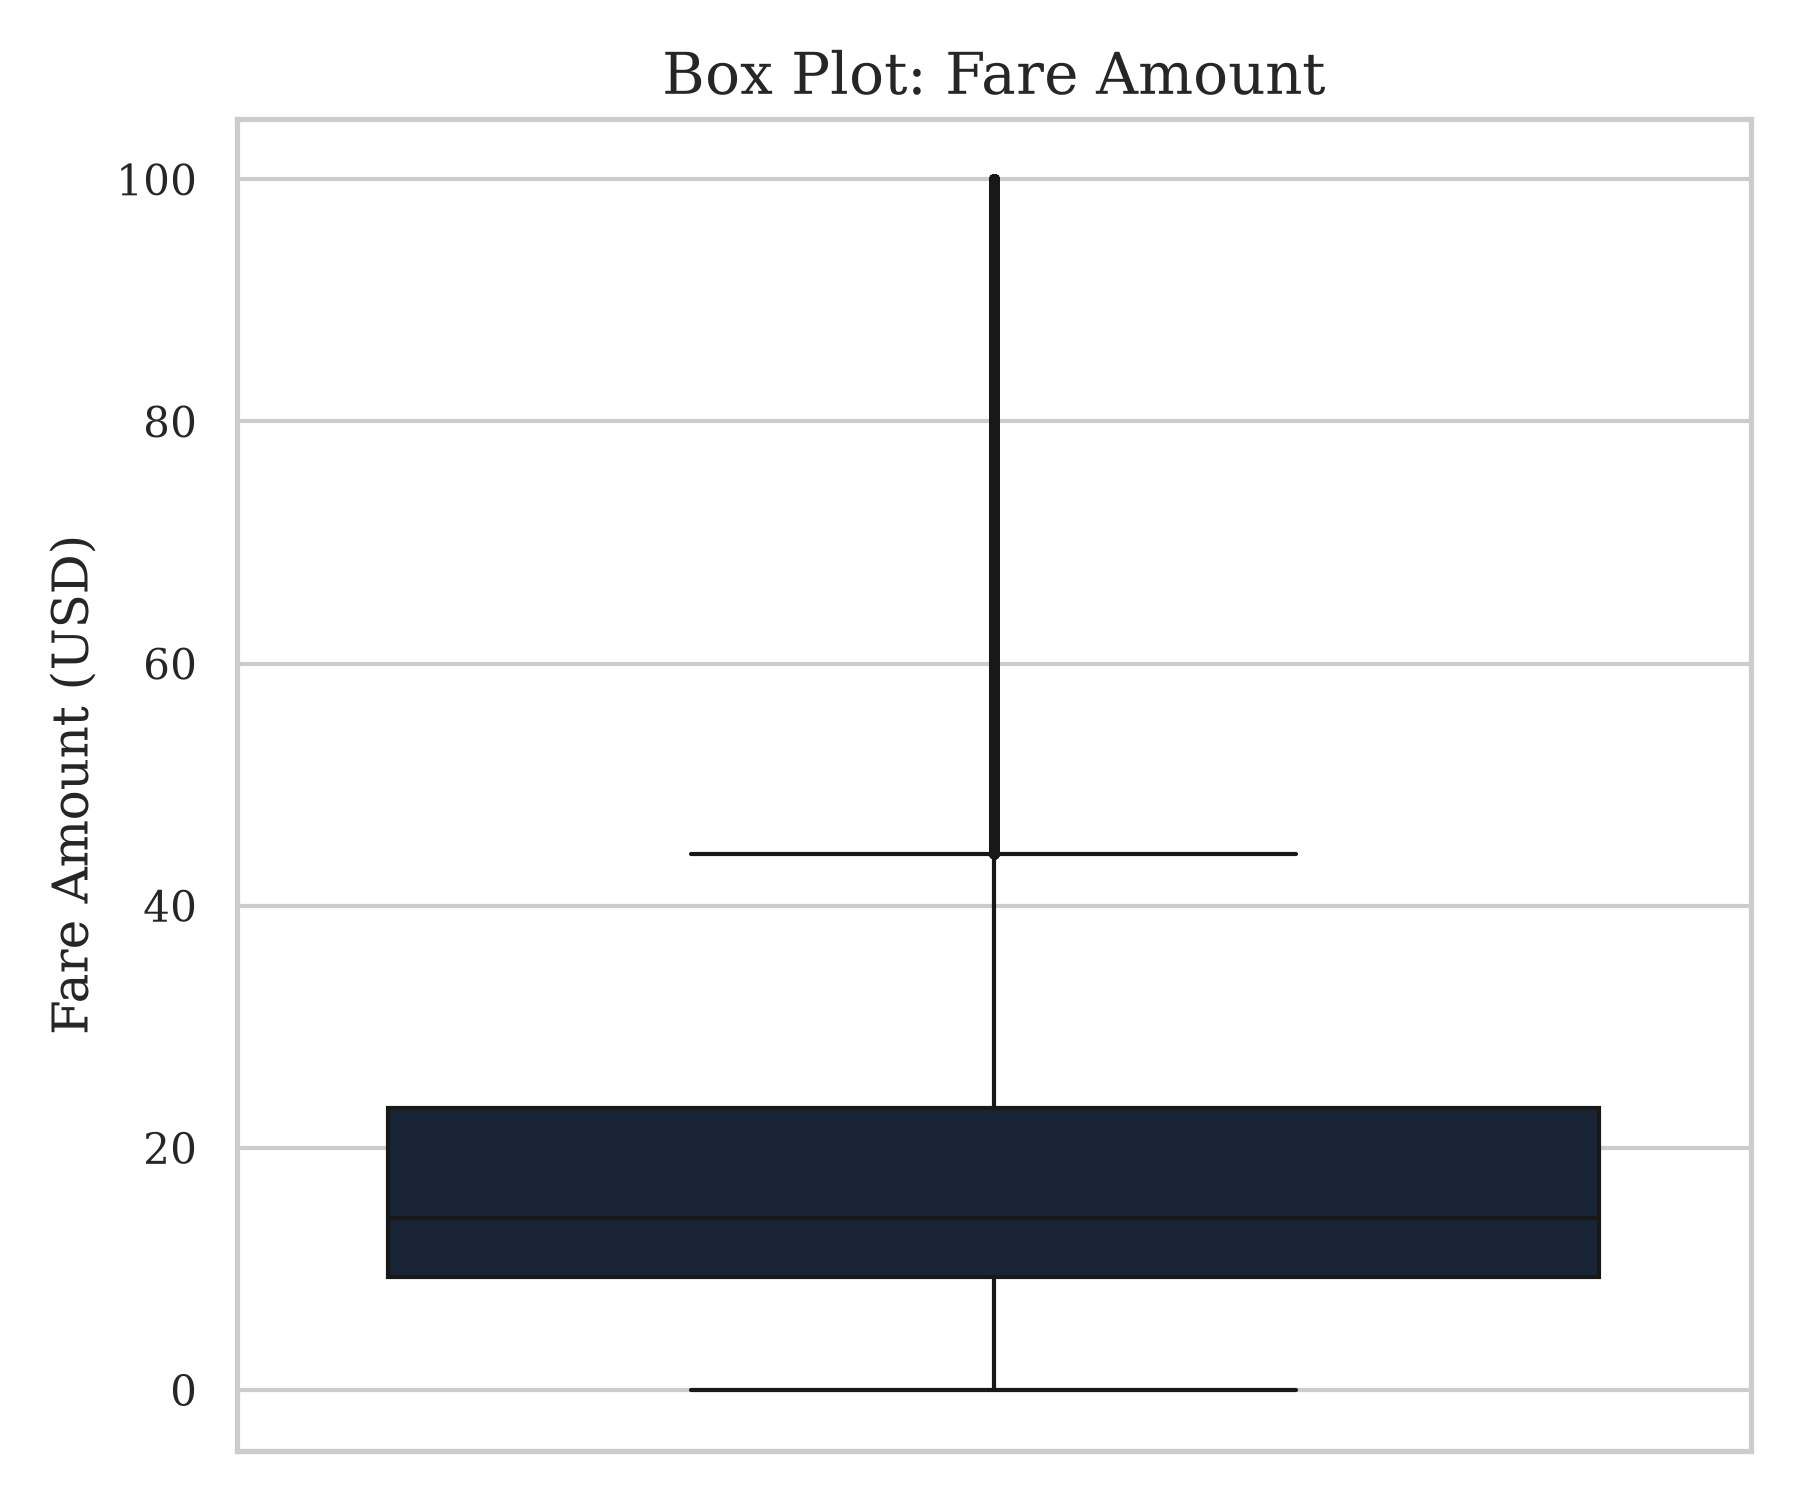
\includegraphics[width=\textwidth]{../figures/fare_amount_boxplot.png}
        \caption{Box Plot (Capped at \$100)}
        \label{fig:fare_amount_box}
    \end{subfigure}
    \caption{Distribution and Box Plot Analysis for Fare Amount (2025)}
    \label{fig:fare_amount_analysis}
\end{figure}

\subsubsection{Justification for Retaining Outliers Beyond the 1.5$\times$IQR Rule}
Under standard Tukey fence criteria, the upper bound for outliers is defined as $Q_3 + 1.5 \times \text{IQR}$. Given an approximate third quartile $Q_3 = \$23.30$ and an IQR of $\$14.00$, this traditional threshold flags any fare exceeding approximately $\$44.30$ as an outlier.

However, \textbf{these high-value fare observations are strictly retained rather than trimmed} for the following operational and economic reasons:
\begin{enumerate}
    \item \textbf{Commercial Validity of Airport Flat Rates:} Fares exceeding the $\$44.30$ threshold are not data errors or anomalies; they represent authorized high-value commercial transactions, most notably the regulated flat rates for trips between Manhattan and major regional airports ($\approx \$70$, clearly visible in Figure~\ref{fig:fare_amount_dist}). Deleting these records would discard crucial airport demand data.
    \item \textbf{Prevention of Economic Distortion:} Trimming observations beyond the $1.5 \times \text{IQR}$ fence would artificially deflate total revenue estimates, average ticket sizes, and macro-economic metrics across the dataset. Retaining them preserves the true economic distribution of NYC yellow taxi operations.
    \item \textbf{Robust Analytical Presentation:} Rather than destructive data filtering, extreme financial values are managed through robust location-and-spread metrics (median and IQR) and visual capping ($\$100$ ceiling in Figure~\ref{fig:fare_amount_box}) to ensure graphical readability while maintaining complete data fidelity.
\end{enumerate}

\subsection{Exploratory Data Analysis: Central Business District Congestion Fee}
\label{sec:eda_cbd_congestion_fee}

The \texttt{cbd\_congestion\_fee} variable captures the Central Business District (CBD) congestion toll structure introduced across Manhattan's commercial core. Comparing the statistical properties of the fee before and after data cleansing illustrates the structural stability of this policy-mandated variable.

\begin{table}[htbp]
\centering
\caption{Pre- and Post-Cleansing Descriptive Statistics for CBD Congestion Fee (2025 Dataset)}
\label{tab:stats_cbd_congestion_fee_comparison}
\small
\begin{tabular}{lrr}
\toprule
\textbf{Metric} & \textbf{Pre-Cleansing (Raw)} & \textbf{Post-Cleansing (Clean)} \\
\midrule
Total Records ($N$) & 48,722,602 & 44,015,208 \\
Mean ($\mu$) & \$0.53 & \$0.55 \\
25th Percentile ($Q_1$) & \$0.00 & \$0.00 \\
Median ($Q_2$) & \$0.75 & \$0.75 \\
75th Percentile ($Q_3$) & \$0.75 & \$0.75 \\
Standard Deviation ($\sigma$) & \$0.36 & \$0.33 \\
Interquartile Range (IQR) & \$0.75 & \$0.75 \\
Skewness & -1.19 & -1.04 \\
\bottomrule
\end{tabular}
\end{table}

\subsubsection{Statistical Characteristics and Cleansing Impact Analysis}
As detailed in Table~\ref{tab:stats_cbd_congestion_fee_comparison}, the median ($Q_2$) and 75th percentile ($Q_3$) remain perfectly stable at $\$0.75$ across both raw and filtered datasets, while the mean fee adjusts slightly from $\$0.53$ to $\$0.55$. 
\begin{itemize}
    \item \textbf{Impact of Cleansing:} The minor upward shift in the mean fee results from removing unmapped locations and administrative anomalies (such as Zone 264 records) where toll flags were skewed or unrecorded. Filtering these noise entries yields a cleaner representation of core commercial operations.
    \item \textbf{Negative Skewness:} The negative skewness ($-1.04$) denotes a distribution dominated by the upper discrete fee tier.
\end{itemize}

\begin{figure}[htbp]
    \centering
    \begin{subfigure}[b]{0.48\textwidth}
        \centering
        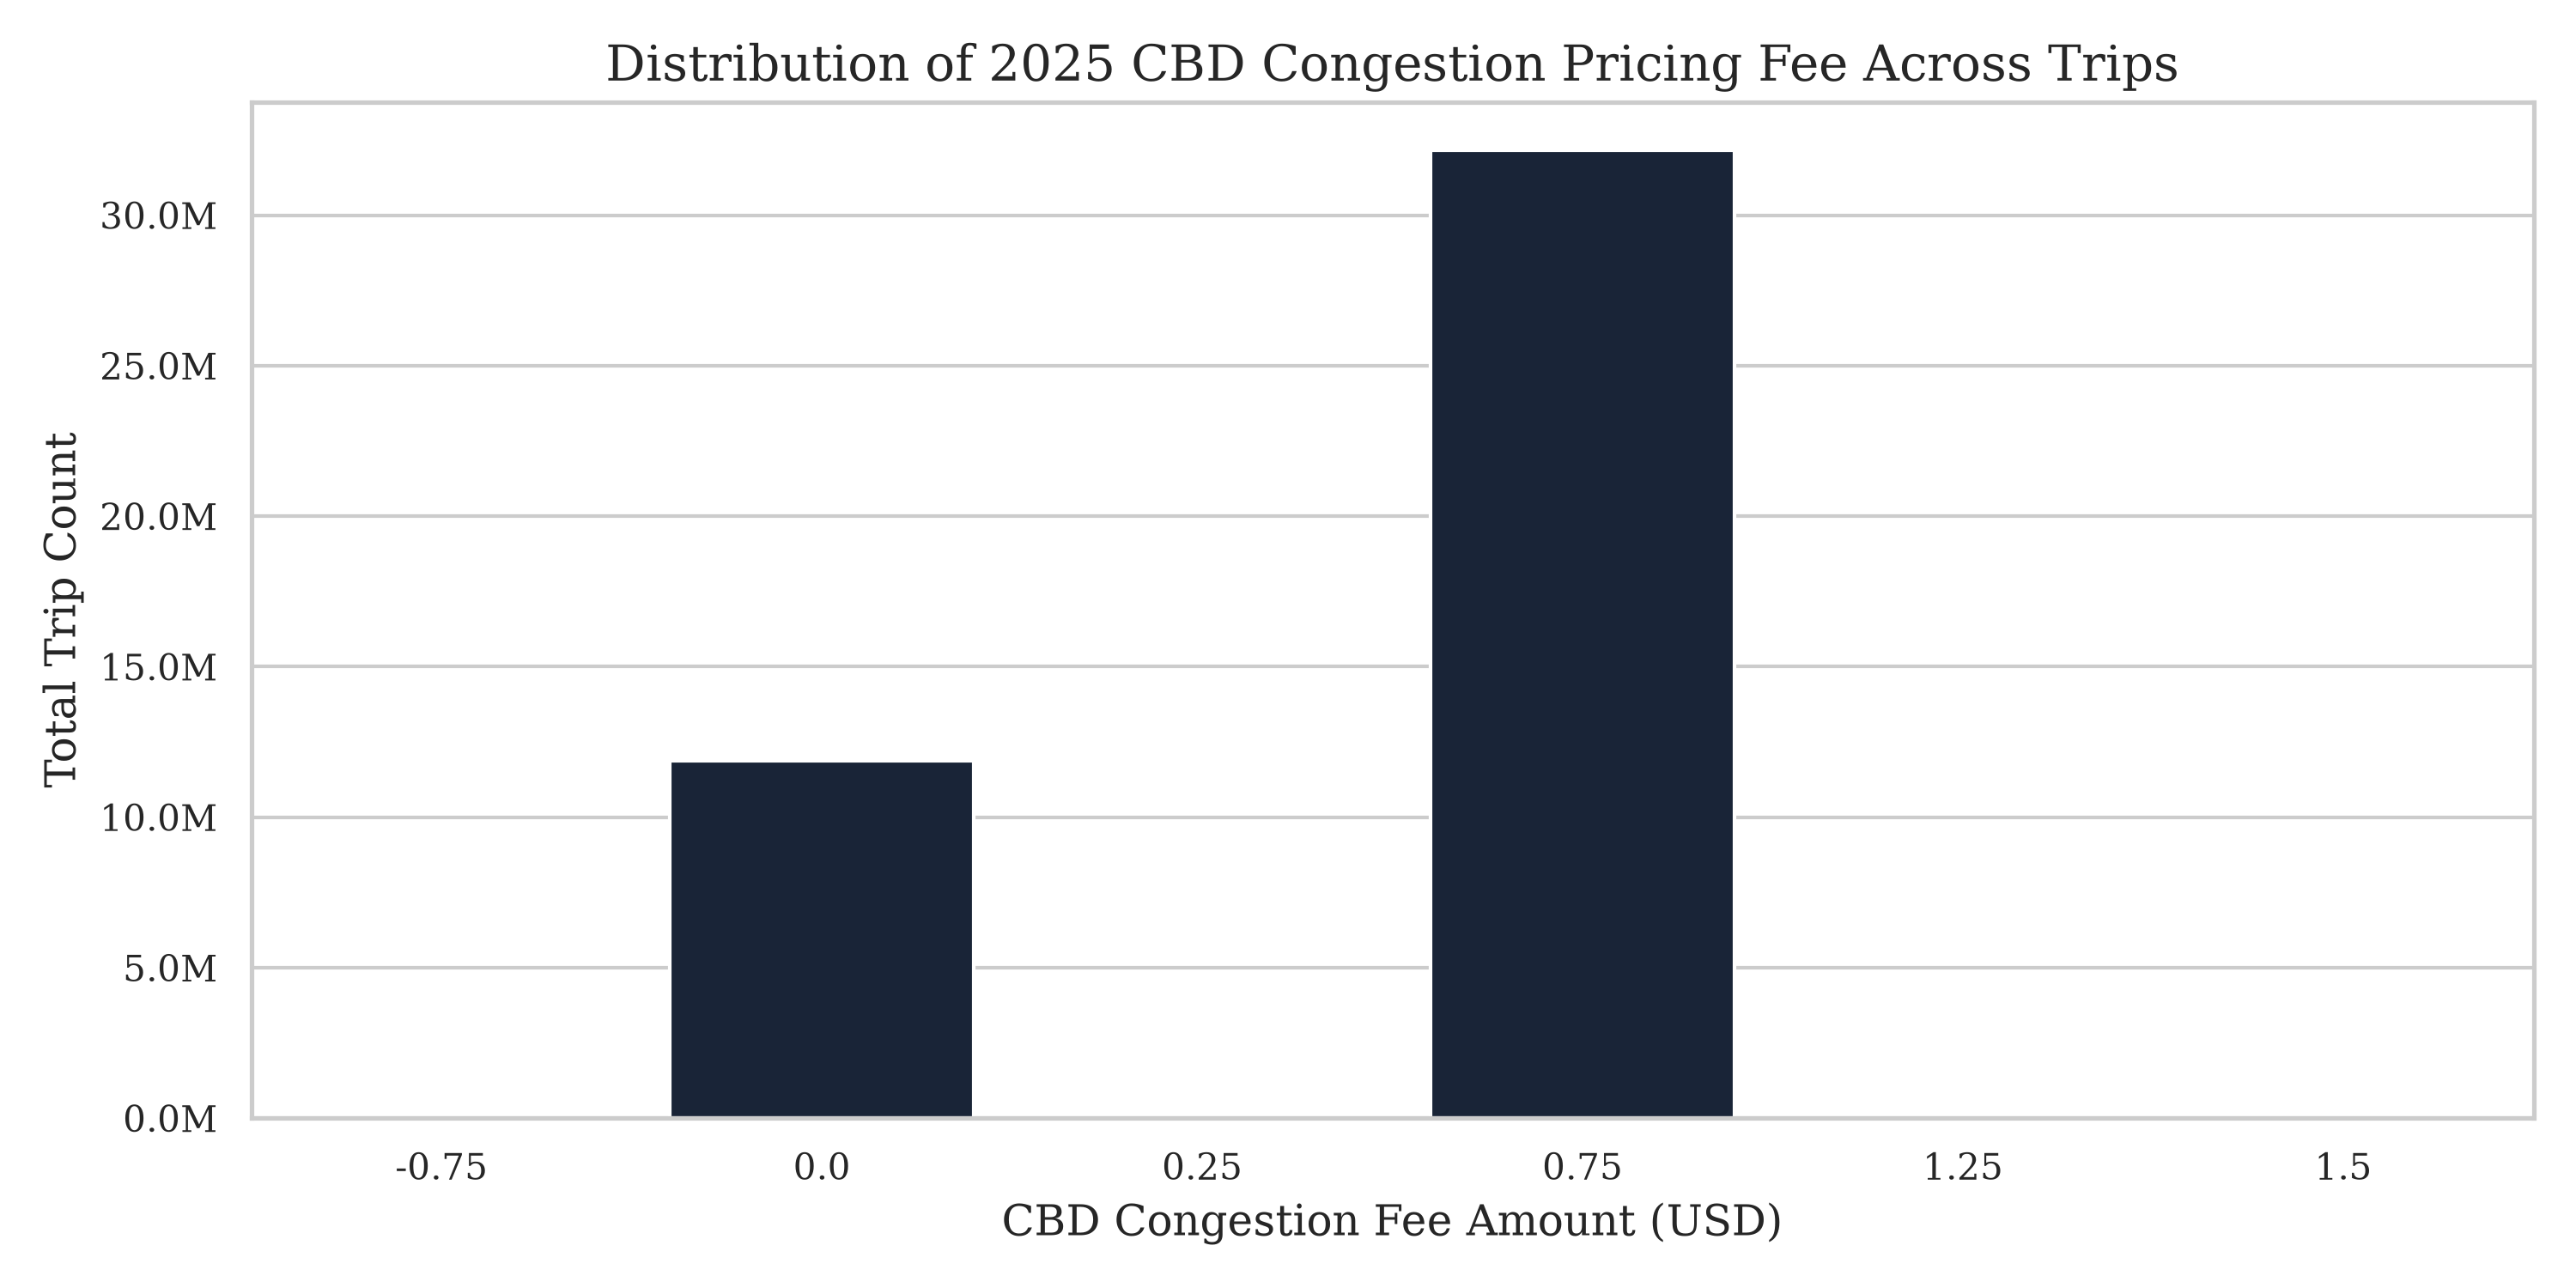
\includegraphics[width=\textwidth]{../figures/cbd_congestion_fee_distribution.png}
        \caption{Frequency Distribution across Fee Tiers}
        \label{fig:cbd_congestion_fee_dist}
    \end{subfigure}
    \hfill
    \begin{subfigure}[b]{0.48\textwidth}
        \centering
        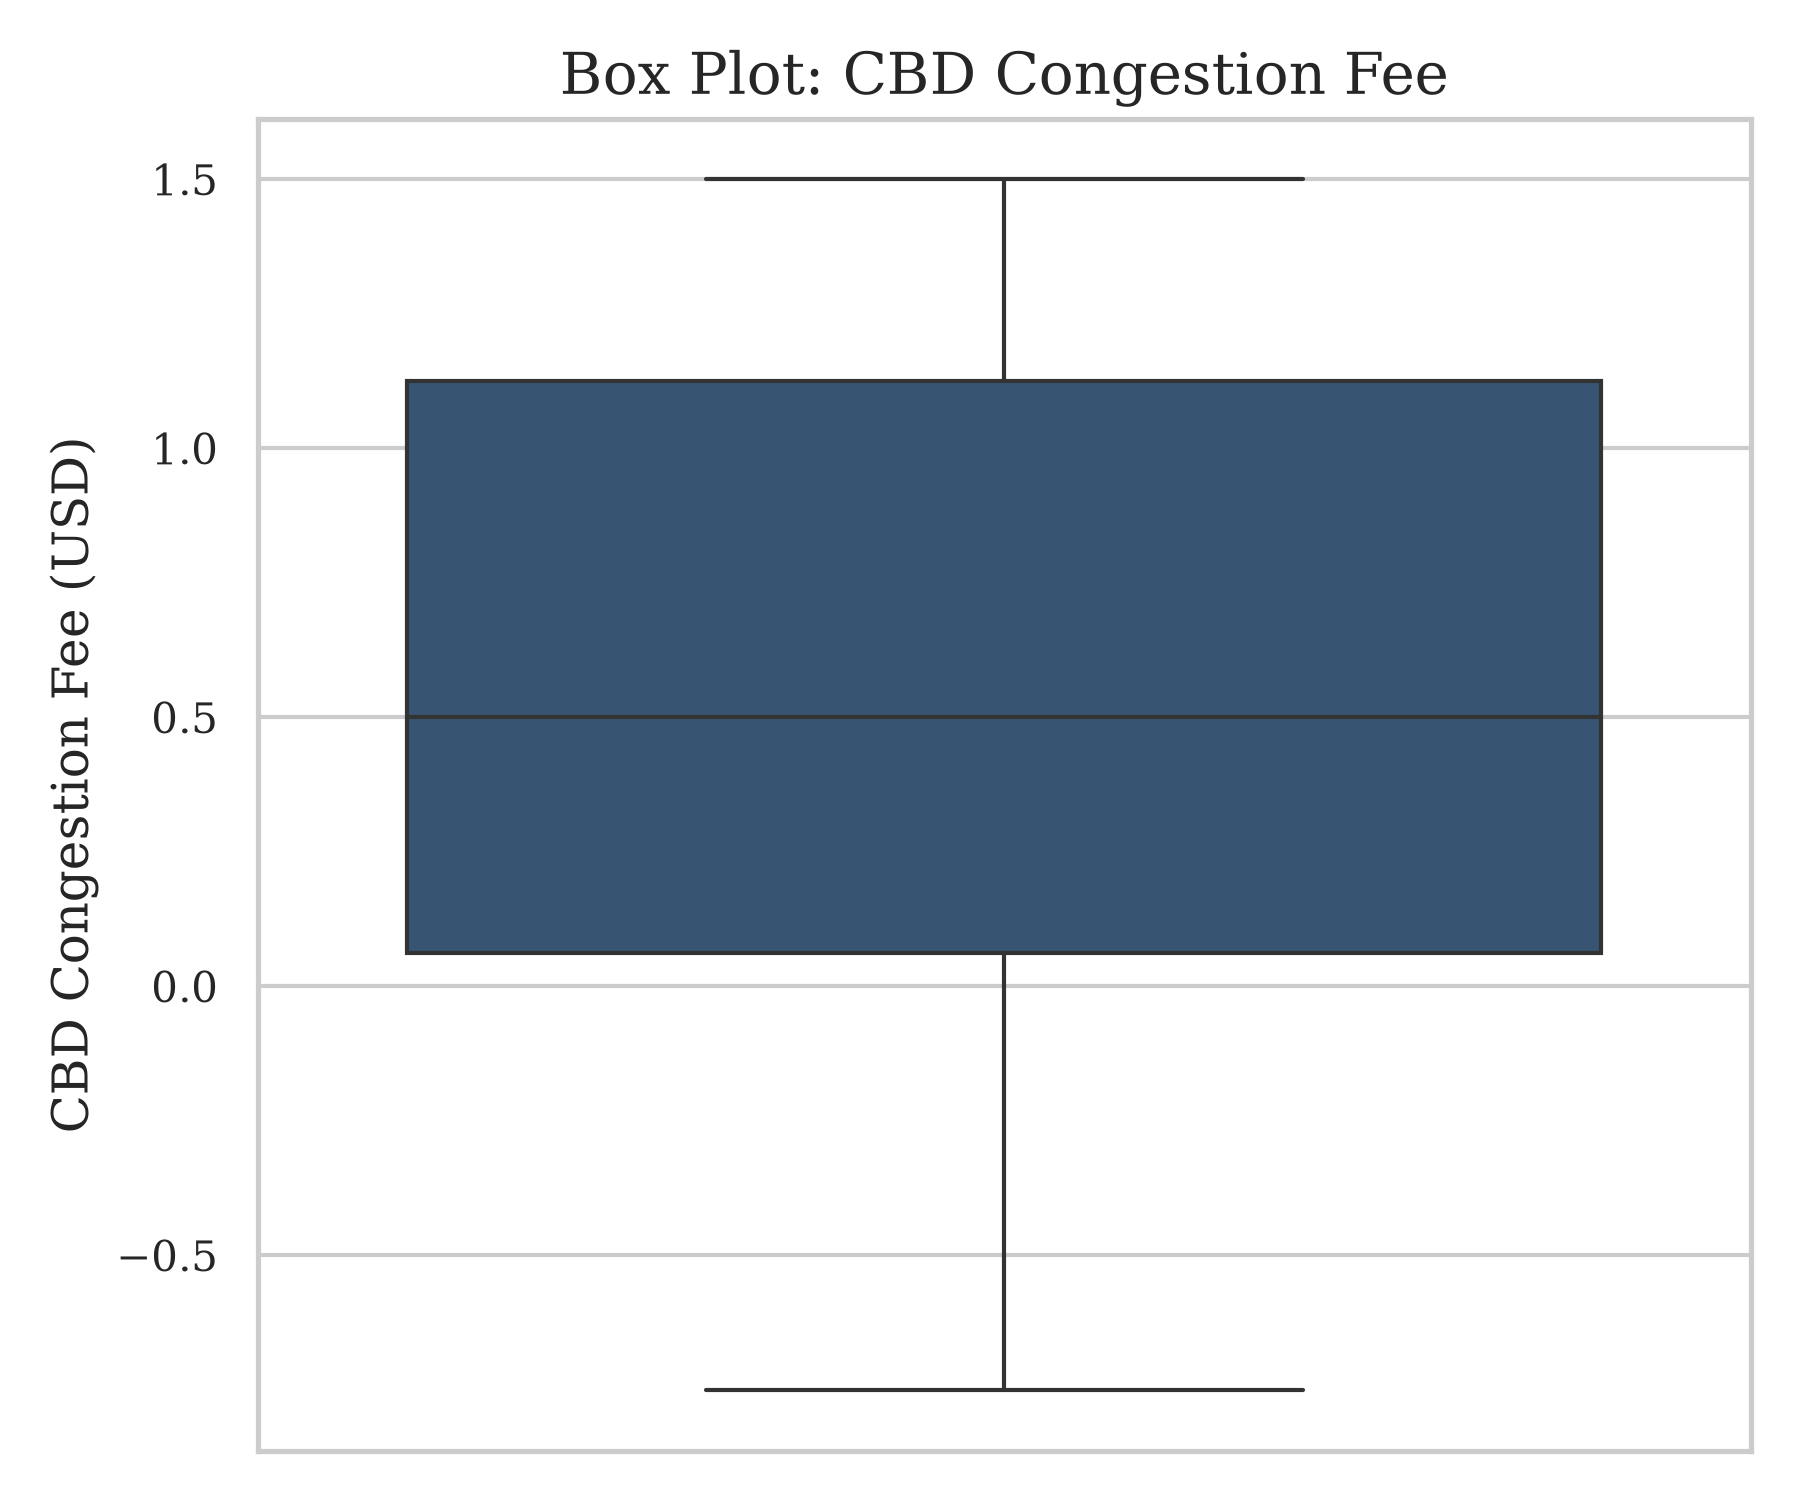
\includegraphics[width=\textwidth]{../figures/cbd_congestion_fee_boxplot.png}
        \caption{Box Plot for Discrete Policy Levels}
        \label{fig:cbd_congestion_fee_box}
    \end{subfigure}
    \caption{Distribution and Box Plot Analysis for CBD Congestion Fee (2025)}
    \label{fig:cbd_congestion_fee_analysis}
\end{figure}

Unlike continuous distance or fare measures, the fee follows a strict, highly concentrated discrete distribution (Figure~\ref{fig:cbd_congestion_fee_dist}):
\begin{enumerate}
    \item \textbf{Active Congestion Toll Tier ($\$0.75$):} Captures approximately $32.1$ million trips (over $73\%$ of total fleet volume), corresponding to journeys entering, exiting, or operating entirely within the designated Manhattan CBD zone.
    \item \textbf{Exempt/Non-Zone Tier ($\$0.00$):} Accounted for by roughly $11.9$ million trips ($\approx 27\%$), representing outer-borough trips or movements operating outside the congestion perimeter.
\end{enumerate}

\subsubsection{Data Integrity and Analytical Interpretation}
Because \texttt{cbd\_congestion\_fee} represents a policy-mandated discrete regulatory toll, standard continuous outlier filtering methods (such as Tukey's $1.5 \times \text{IQR}$ rule) do not apply. As displayed in the box plot (Figure~\ref{fig:cbd_congestion_fee_box}), the distribution spans bounded policy levels without arbitrary extreme points. Retaining both $\$0.00$ and $\$0.75$ values is essential for evaluating fleet policy compliance, revenue collection accuracy, and spatial traffic impacts within Manhattan's core.
\subsection{Exploratory Data Analysis: Passenger Count}
\label{sec:eda_passenger_count}

The \texttt{passenger\_count} variable tracks the number of passengers reported by the driver during the trip. Across the 2025 dataset, while unrecorded or missing passenger entries account for $11,611,894$ records ($23.83\%$ of total raw volume), the subset of valid, explicitly recorded trips comprises $35,174,850$ records. Passenger occupancy patterns across this valid subset demonstrate the heavy prevalence of single-occupancy transit typical of urban yellow taxi services.

\begin{table}[htbp]
\centering
\caption{Descriptive Statistics for Valid Passenger Count (2025 Dataset)}
\label{tab:stats_passenger_count}
\begin{tabular}{lr}
\toprule
\textbf{Metric} & \textbf{Value} \\
\midrule
Total Valid Recorded Trips & 35,174,522 \\
Mode & 1 \\
Mean ($\mu$) & 1.29 \\
25th Percentile ($Q_1$) & 1.00 \\
Median ($Q_2$) & 1.00 \\
75th Percentile ($Q_3$) & 1.00 \\
Standard Deviation ($\sigma$) & 0.72 \\
Interquartile Range (IQR) & 0.00 \\
Skewness & 2.97 \\
\bottomrule
\end{tabular}
\end{table}

\subsubsection{Statistical Characteristics and Distribution Shape}
As summarized in Table~\ref{tab:stats_passenger_count}, for the subset of explicitly recorded trips, the mode, 25th percentile ($Q_1$), median ($Q_2$), and 75th percentile ($Q_3$) are all strictly $1.00$, with a mean ($\mu$) of $1.29$ and an IQR of $0.00$ due to the overwhelming concentration of single-passenger rides. The distribution exhibits a positive skewness of $2.97$.

\begin{figure}[htbp]
    \centering
    \begin{minipage}[b]{0.48\textwidth}
        \centering
        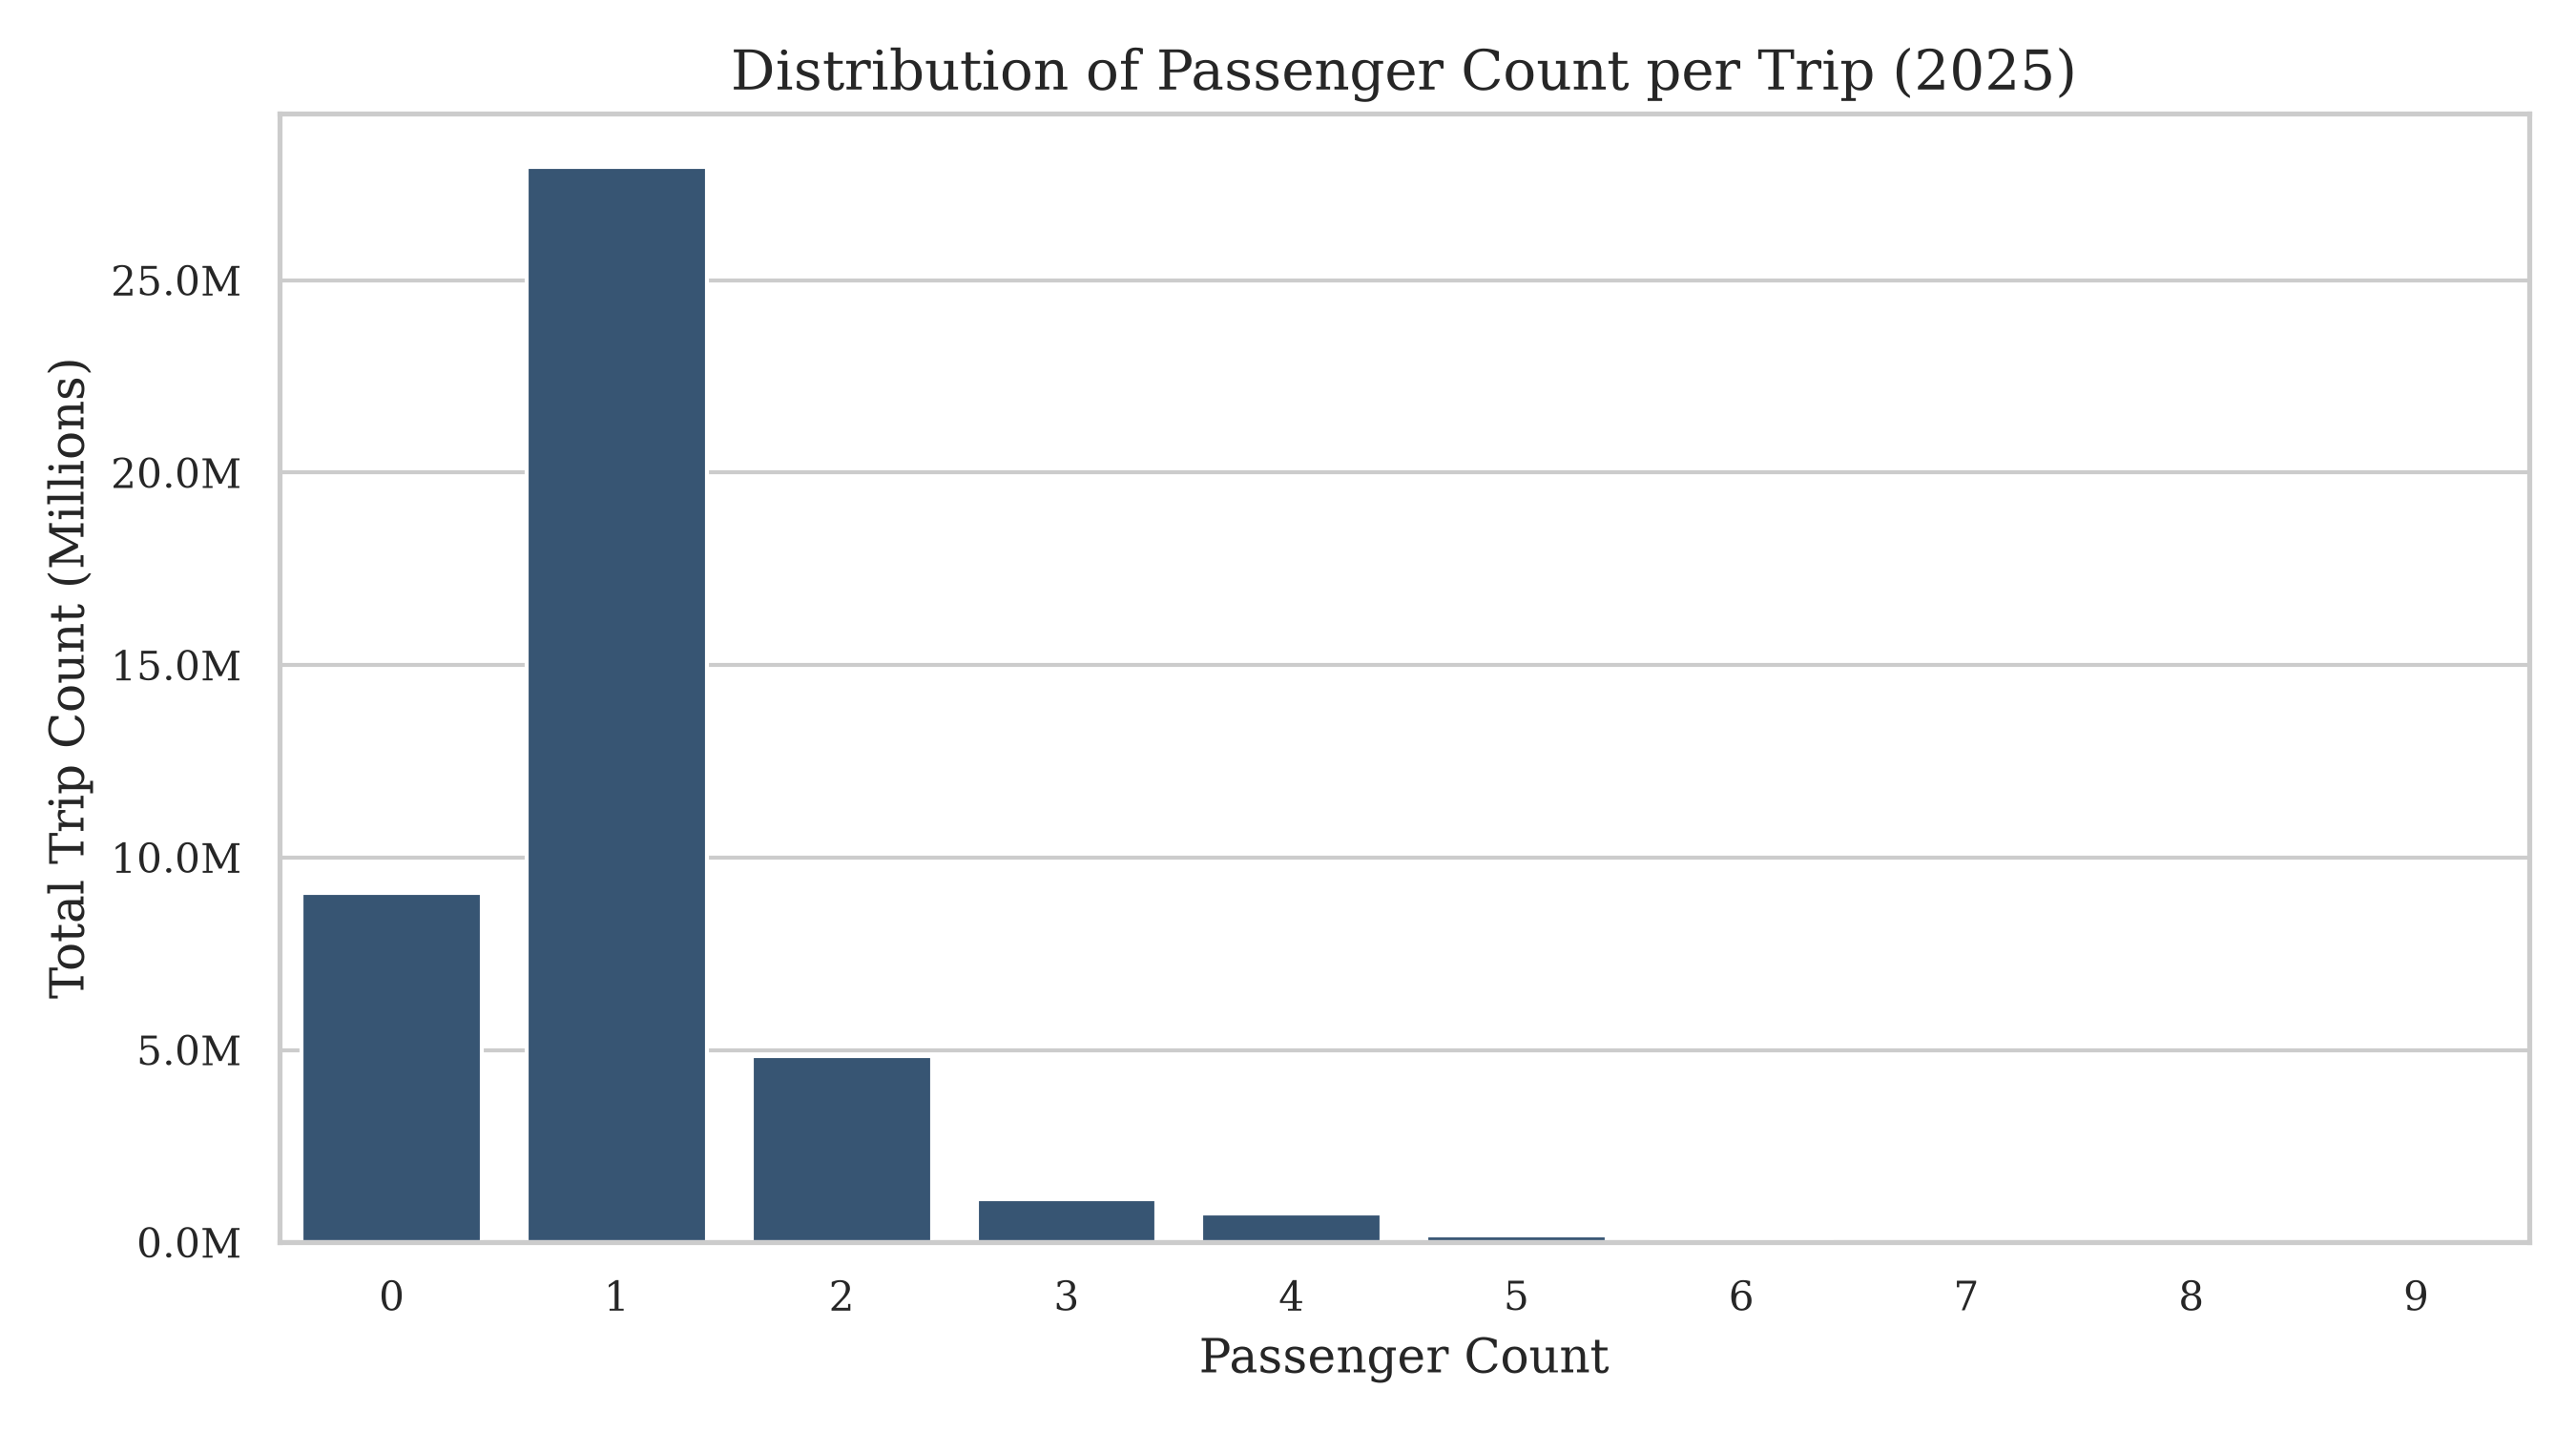
\includegraphics[width=\textwidth]{../figures/passenger_count_distribution.png}
        \caption{Trip Count by Passenger Occupancy (Excluding Unrecorded Values)}
        \label{fig:passenger_count_dist}
    \end{minipage}
    \hfill
    \begin{minipage}[b]{0.48\textwidth}
        \centering
        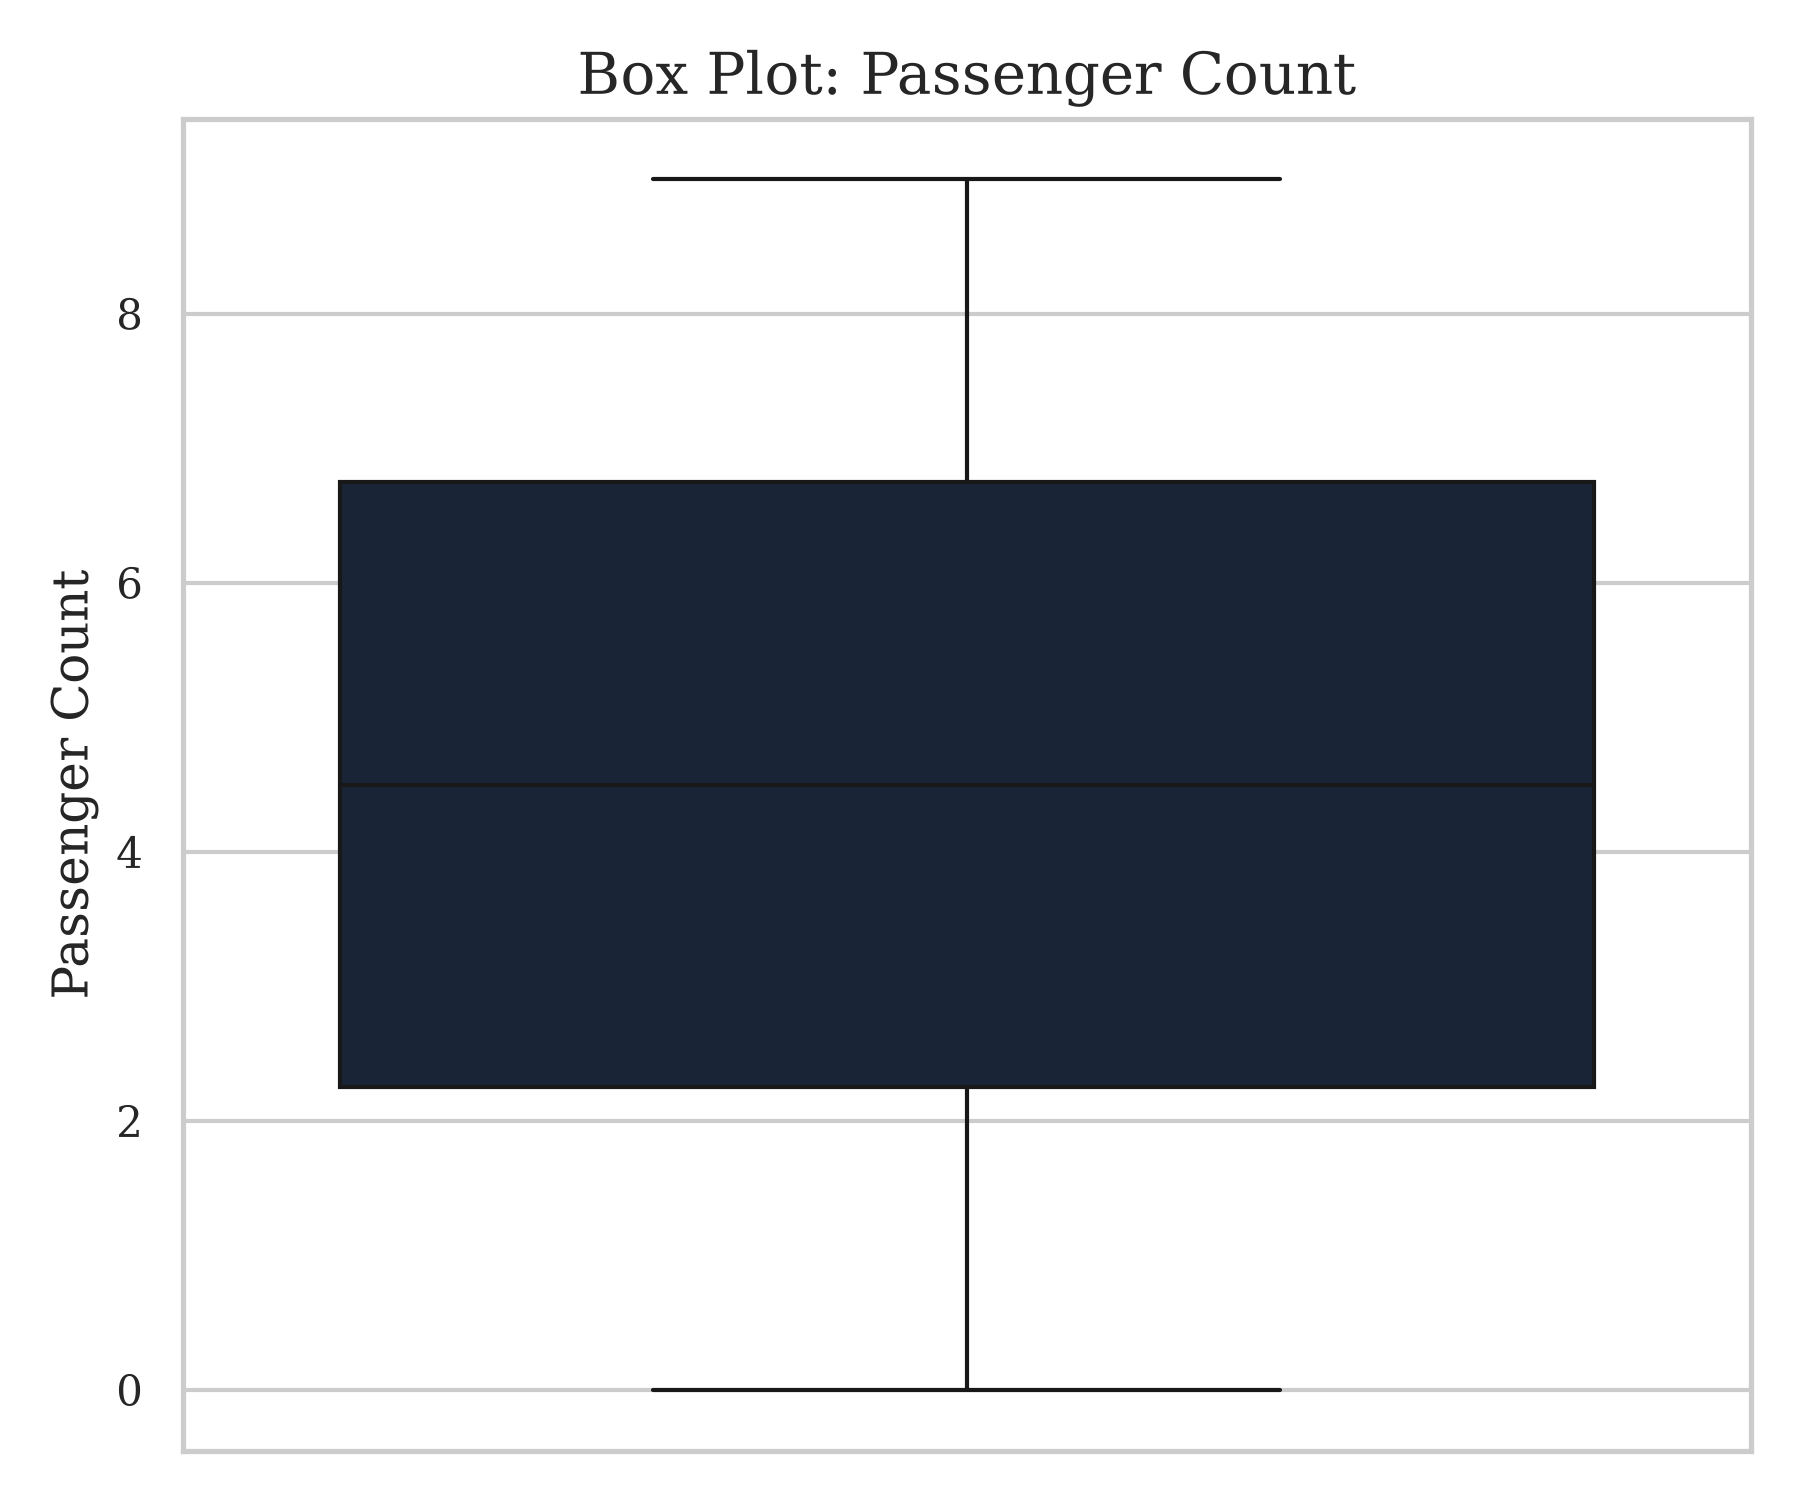
\includegraphics[width=\textwidth]{../figures/passenger_count_boxplot.png}
        \caption{Box Plot for Discrete Occupancy Tiers}
        \label{fig:passenger_count_box}
    \end{minipage}
    \caption{Distribution and Box Plot Analysis for Passenger Count (2025)}
    \label{fig:passenger_count_analysis}
\end{figure}

As visualized in the frequency distribution (Figure~\ref{fig:passenger_count_dist}), which excludes the $11,611,894$ unrecorded or missing entries to ensure clean graphical representation, passenger counts follow a discrete categorical distribution where:
\begin{enumerate}
    \item \textbf{Single Occupancy (1 Passenger):} Dominates fleet utilization, representing the vast majority of recorded trips.
    \item \textbf{Solo/Zero-Passenger Records ($0$ Passengers):} Account for a secondary cluster of trips, typically representing administrative entries, driver-only transits, or unassigned meter logs permitted under TLC guidelines.
    \item \textbf{Multi-Passenger Tiers:} Frequencies drop off sharply for groups of $2$, $3$, $4$, and $5+$ passengers, reflecting physical vehicle capacity limits and typical party sizes for standard yellow cabs.
\end{enumerate}

\subsubsection{Methodological Note on Discrete Categorical Variables and Graphical Exclusions}
Because \texttt{passenger\_count} is an integer-based discrete variable rather than a continuous metric, traditional outlier bounds like Tukey's $1.5 \times \text{IQR}$ rule do not apply in the standard continuous sense. Furthermore, unrecorded and missing passenger count records ($23.83\%$ of the raw dataset) are explicitly excluded from both the frequency distribution plot (Figure~\ref{fig:passenger_count_dist}) and the box plot (Figure~\ref{fig:passenger_count_box}) to prevent null or undefined categories from distorting the visual analysis of active passenger occupancy. Retaining these records in the broader data pipeline while isolating them from univariate graphical rendering ensures both comprehensive data retention and precise visual interpretation.

\subsection{Exploratory Data Analysis: Tip Amount}
\label{sec:eda_tip_amount}

The \texttt{tip\_amount} variable records the gratuity provided by the passenger, automatically captured for electronic payments and optionally logged for cash transactions. Comparing the statistical properties of the tip amount before and after data cleansing illustrates the structural impact of removing gross anomalies.

\begin{table}[htbp]
\centering
\caption{Pre- and Post-Cleansing Descriptive Statistics for Tip Amount (2025 Dataset)}
\label{tab:stats_tip_amount_comparison}
\small
\begin{tabular}{lrr}
\toprule
\textbf{Metric} & \textbf{Pre-Cleansing (Raw)} & \textbf{Post-Cleansing (Clean)} \\
\midrule
Total Records ($N$) & 48,722,602 & 44,015,208 \\
Mean ($\mu$) & \$2.84 & \$3.04 \\
25th Percentile ($Q_1$) & \$0.00 & \$0.00 \\
Median ($Q_2$) & \$2.00 & \$2.39 \\
75th Percentile ($Q_3$) & \$3.99 & \$4.07 \\
Standard Deviation ($\sigma$) & \$3.97 & \$3.96 \\
Interquartile Range (IQR) & \$3.99 & \$4.07 \\
Skewness & 5.28 & 4.53 \\
\bottomrule
\end{tabular}
\end{table}

\subsubsection{Statistical Characteristics and Cleansing Impact Analysis}
As summarized in Table~\ref{tab:stats_tip_amount_comparison}, the median tip shifts from $\$2.00$ in the raw dataset to $\$2.39$ after cleaning, while the mean increases from $\$2.84$ to $\$3.04$. 
\begin{itemize}
    \item \textbf{Impact of Cleansing:} The upward adjustment in both median and mean gratuities stems from filtering out unmapped or erroneous records (such as negative-fare dispute reversals and zero-distance system tests) that corrupted financial reporting. Removing these distortions yields a cleaner representation of true passenger tipping behavior.
    \item \textbf{Distributional Shape:} The distribution continues to exhibit strong positive skewness ($4.53$) and significant dispersion ($\sigma = \$3.96$).
\end{itemize}

The probability density function (Figure~\ref{fig:tip_amount_dist}) reveals a distinct zero-inflated structure, characterized by a massive spike at $\$0.00$. This prominent zero-inflation corresponds primarily to cash-paid trips (where gratuities are handed directly to drivers and unrecorded digitally) as well as zero-tip credit card transactions. Beyond the zero origin, the distribution forms a smooth right-skewed hump peaking between $\$2.00$ and $\$3.00$, accompanied by minor multimodal bumps at round currency increments (such as $\$10.00$ and $\$15.00$) representing fixed or percentage-based gratuities on longer journeys.

\begin{figure}[htbp]
    \centering
    \begin{subfigure}[b]{0.48\textwidth}
        \centering
        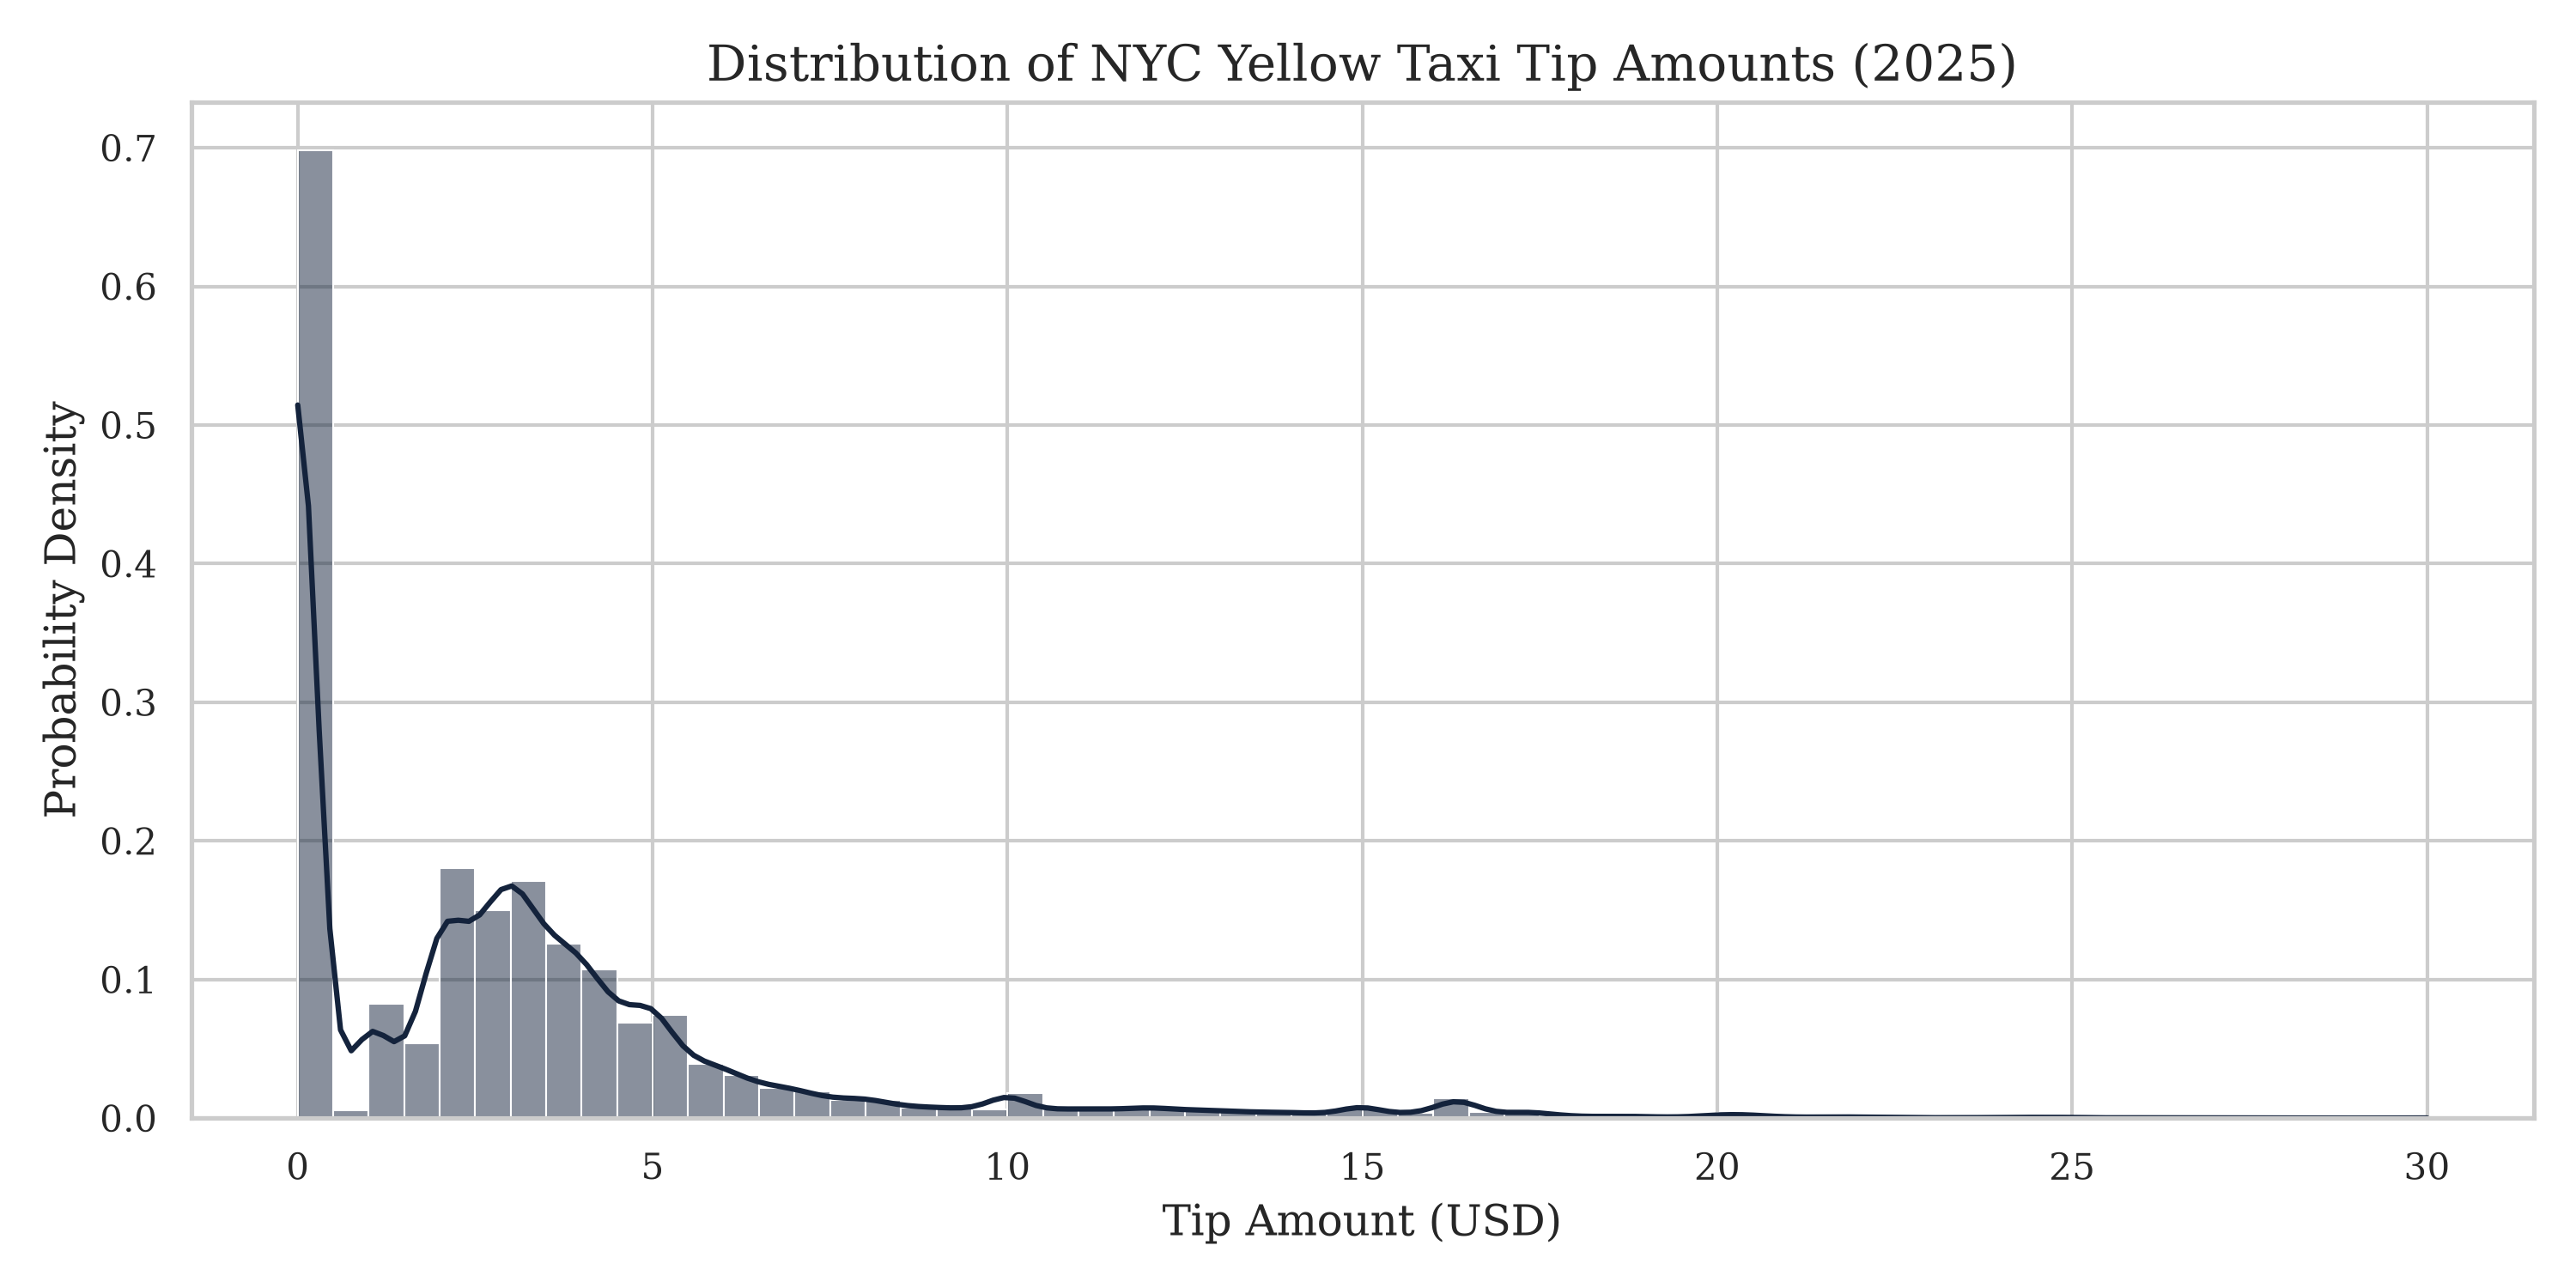
\includegraphics[width=\textwidth]{../figures/tip_amount_distribution.png}
        \caption{Probability Density Distribution}
        \label{fig:tip_amount_dist}
    \end{subfigure}
    \hfill
    \begin{subfigure}[b]{0.48\textwidth}
        \centering
        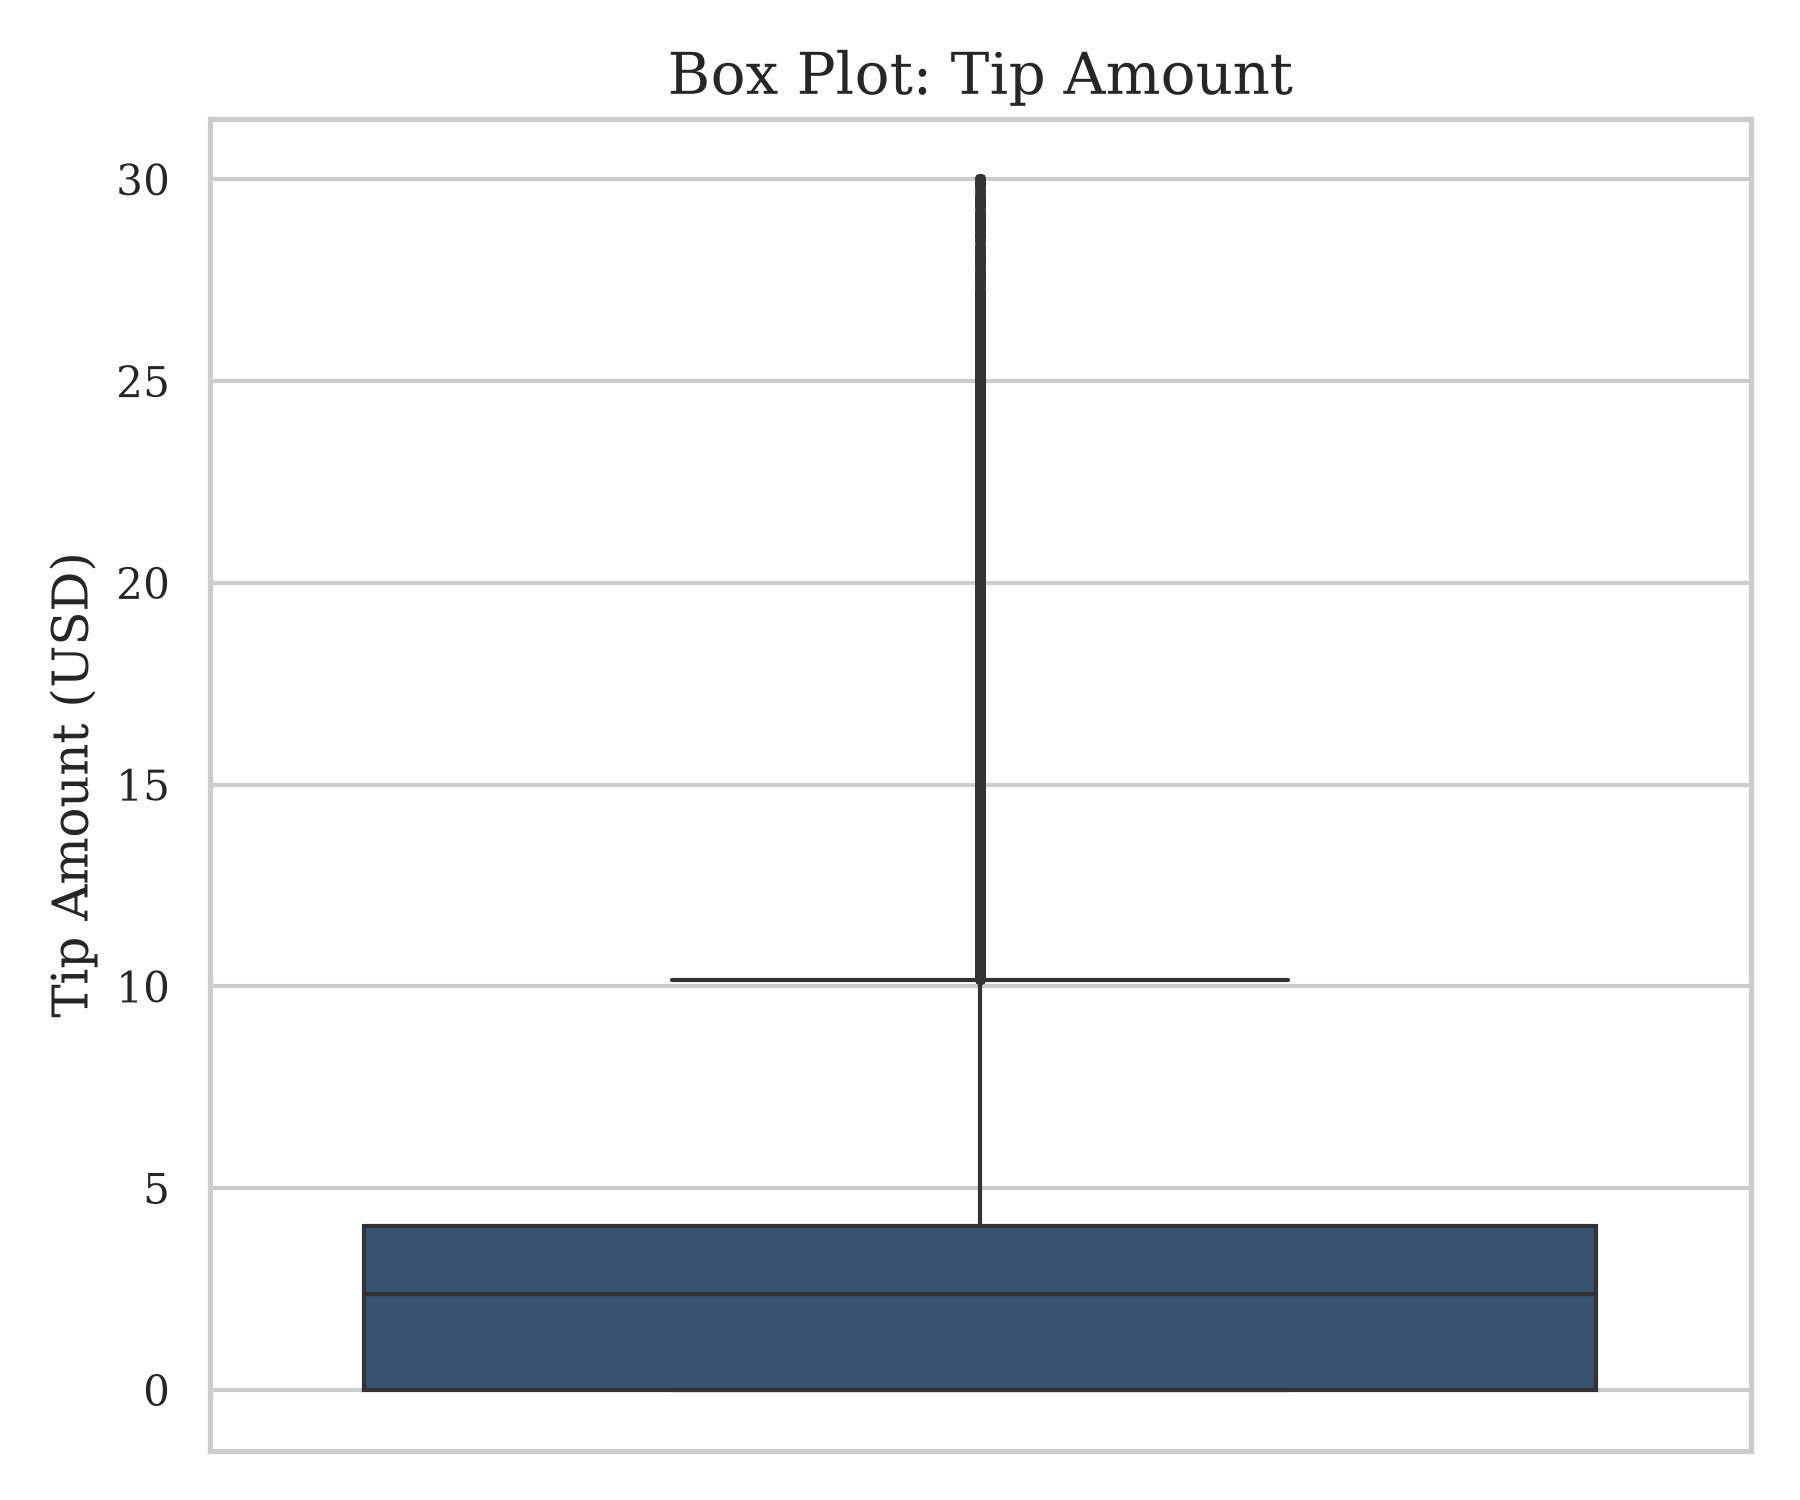
\includegraphics[width=\textwidth]{../figures/tip_amount_boxplot.png}
        \caption{Box Plot (Capped at \$30)}
        \label{fig:tip_amount_box}
    \end{subfigure}
    \caption{Distribution and Box Plot Analysis for Tip Amount (2025)}
    \label{fig:tip_amount_analysis}
\end{figure}

\subsubsection{Justification for Retaining Outliers Beyond the 1.5$\times$IQR Rule}
Under standard Tukey fence criteria, the upper bound for outliers is defined as $Q_3 + 1.5 \times \text{IQR}$. Given a third quartile $Q_3 = \$4.07$ and an IQR of $\$4.07$, this traditional threshold flags any tip exceeding approximately $\$10.175$ as an outlier candidate for removal.

However, \textbf{these high-value tip observations are strictly retained rather than trimmed} for the following operational and economic reasons:
\begin{enumerate}
    \item \textbf{Commercial Validity of Generous Gratuities:} Tips exceeding $\$10.175$—and extending up to the plotted $\$30.00$ ceiling (Figure~\ref{fig:tip_amount_box})—are authentic economic transactions. They typically accompany high-fare airport transfers, long-distance inter-borough trips, or exceptional customer service satisfaction.
    \item \textbf{Prevention of Economic Distortion:} Trimming observations beyond the $1.5 \times \text{IQR}$ fence would artificially depress driver earnings estimations, distort cashless economic modeling, and bias analyses exploring the relationship between fare size and tip generosity.
    \item \textbf{Robust Analytical Presentation:} Rather than destructive data deletion, extreme gratuity values are accommodated through robust summary statistics (median and IQR) and visual capping ($\$30$ ceiling in Figure~\ref{fig:tip_amount_box}) to ensure graphical clarity without sacrificing dataset integrity.
\end{enumerate}

\subsection{Exploratory Data Analysis: Trip Duration}
\label{sec:eda_trip_duration}

The \texttt{trip\_duration\_minutes} variable measures the elapsed travel time in minutes, computed as the exact difference between drop-off and pick-up timestamps ($\Delta t$). Comparing the statistical properties and visual distributions of trip duration before and after data cleansing illustrates the structural impact of removing extreme telemetry and clock-reset anomalies.

\begin{table}[htbp]
\centering
\caption{Pre- and Post-Cleansing Descriptive Statistics for Trip Duration (2025 Dataset)}
\label{tab:stats_trip_duration_comparison}
\small
\begin{tabular}{lrr}
\toprule
\textbf{Metric} & \textbf{Pre-Cleansing (Raw)} & \textbf{Post-Cleansing (Clean)} \\
\midrule
Total Records ($N$) & 48,722,602 & 44,015,208 \\
Mean ($\mu$) & 17.36 minutes & 17.23 minutes \\
25th Percentile ($Q_1$) & 8.12 minutes & 8.30 minutes \\
Median ($Q_2$) & 13.48 minutes & 13.53 minutes \\
75th Percentile ($Q_3$) & 21.48 minutes & 21.52 minutes \\
Standard Deviation ($\sigma$) & 28.29 minutes & 13.82 minutes \\
Interquartile Range (IQR) & 13.37 minutes & 13.22 minutes \\
Skewness & -69.38 & 2.49 \\
\bottomrule
\end{tabular}
\end{table}

\subsubsection{Statistical Characteristics and Cleansing Impact Analysis}
As summarized in Table~\ref{tab:stats_trip_duration_comparison}, data cleansing significantly stabilized the dataset's dispersion and distributional shape:
\begin{itemize}
    \item \textbf{Impact on Dispersion and Variance:} In the raw dataset, extreme clock-reset errors and meters left running for 24+ hours inflated the standard deviation to $28.29$ minutes. Filtering out durations exceeding $240$ minutes and non-positive intervals reduced the standard deviation by over $50\%$ down to $13.82$ minutes.
    \item \textbf{Correction of Skewness:} The raw dataset exhibited a heavily distorted negative skewness ($-69.38$) driven by timestamp anomalies. Removing these errors restored a natural, right-skewed distribution ($\text{Skewness} = 2.49$), reflecting an operational structure dominated by short urban movements coupled with an extended tail of prolonged cross-borough or congested journeys.
\end{itemize}

Visual inspection further highlights this transformation. Figure~\ref{fig:trip_duration_precleansing} displays the raw pre-cleansing distribution, where distortion artifacts and extreme tails obscure core operational patterns. In contrast, the filtered probability density function (Figure~\ref{fig:trip_duration_dist}) and box plot (Figure~\ref{fig:trip_duration_box}) display a smooth, unimodal distribution rising steeply from zero, peaking sharply between $8$ and $12$ minutes (representing standard intra-neighborhood and mid-Manhattan trips), and tapering into a natural right-hand tail corresponding to extended regional commutes.

\begin{figure}[htbp]
    \centering
    \begin{subfigure}[b]{\textwidth}
        \centering
        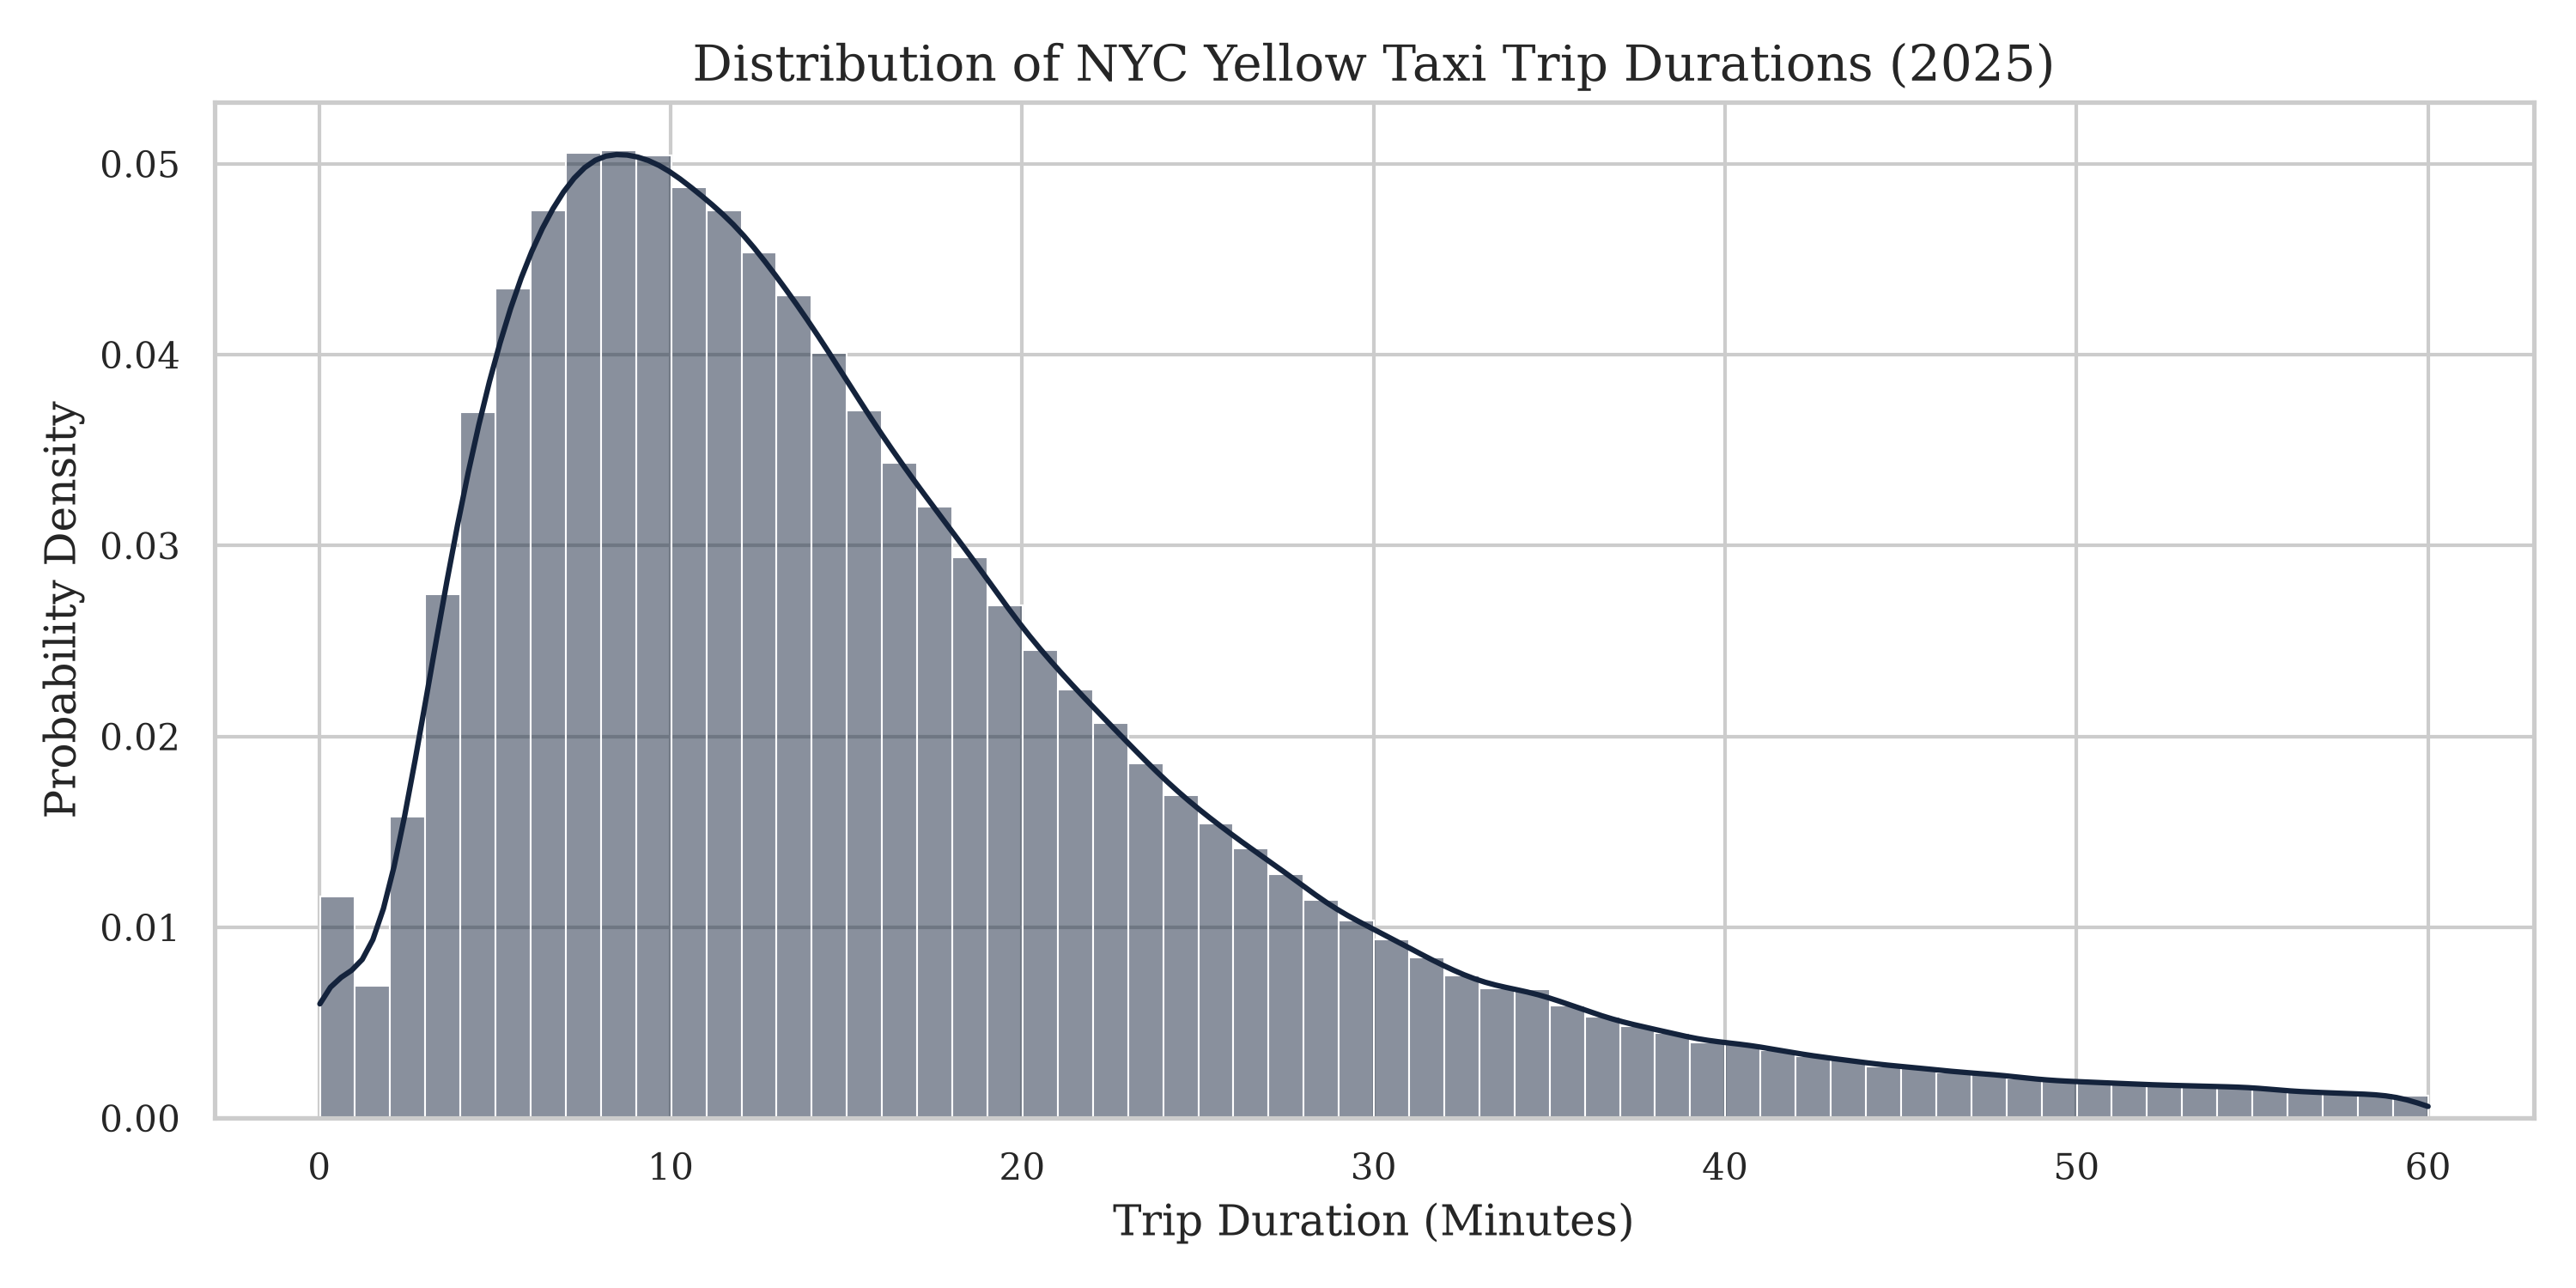
\includegraphics[width=0.85\textwidth]{../figures/trip_duration_distribution_precleansing.png}
        \caption{Pre-Cleansing Trip Duration Distribution (Showing Raw Anomalies)}
        \label{fig:trip_duration_precleansing}
    \end{subfigure}
    \vskip 0.5em
    \begin{subfigure}[b]{0.48\textwidth}
        \centering
        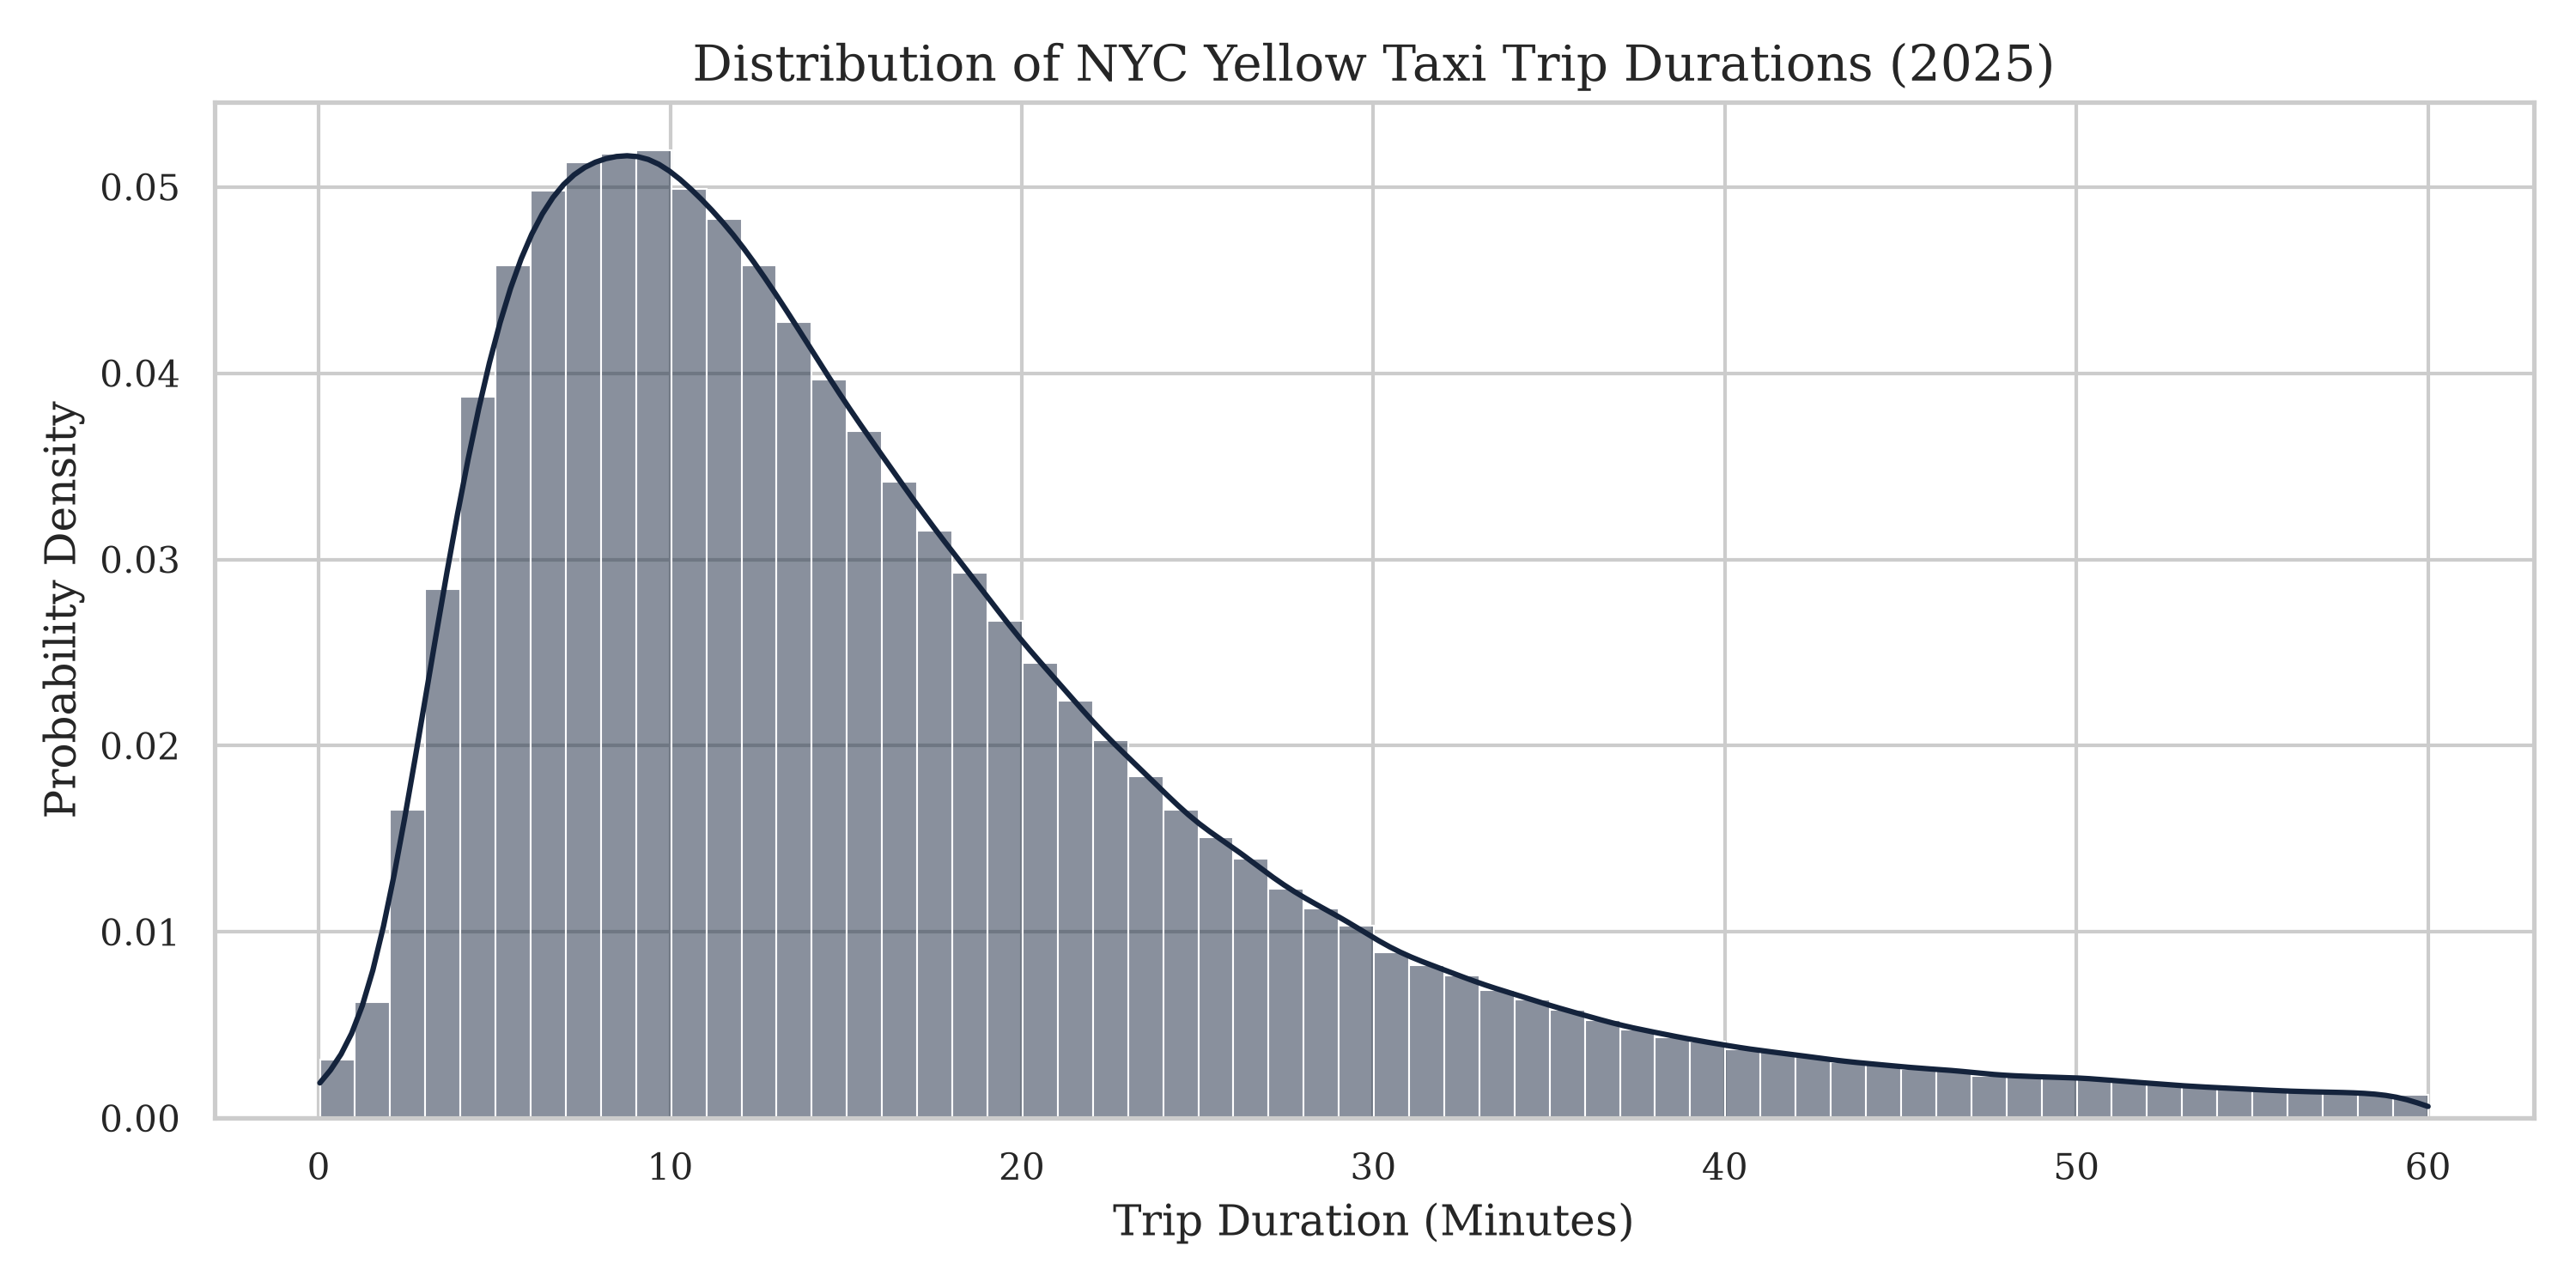
\includegraphics[width=\textwidth]{../figures/trip_duration_distribution.png}
        \caption{Post-Cleansing Probability Density}
        \label{fig:trip_duration_dist}
    \end{subfigure}
    \hfill
    \begin{subfigure}[b]{0.48\textwidth}
        \centering
        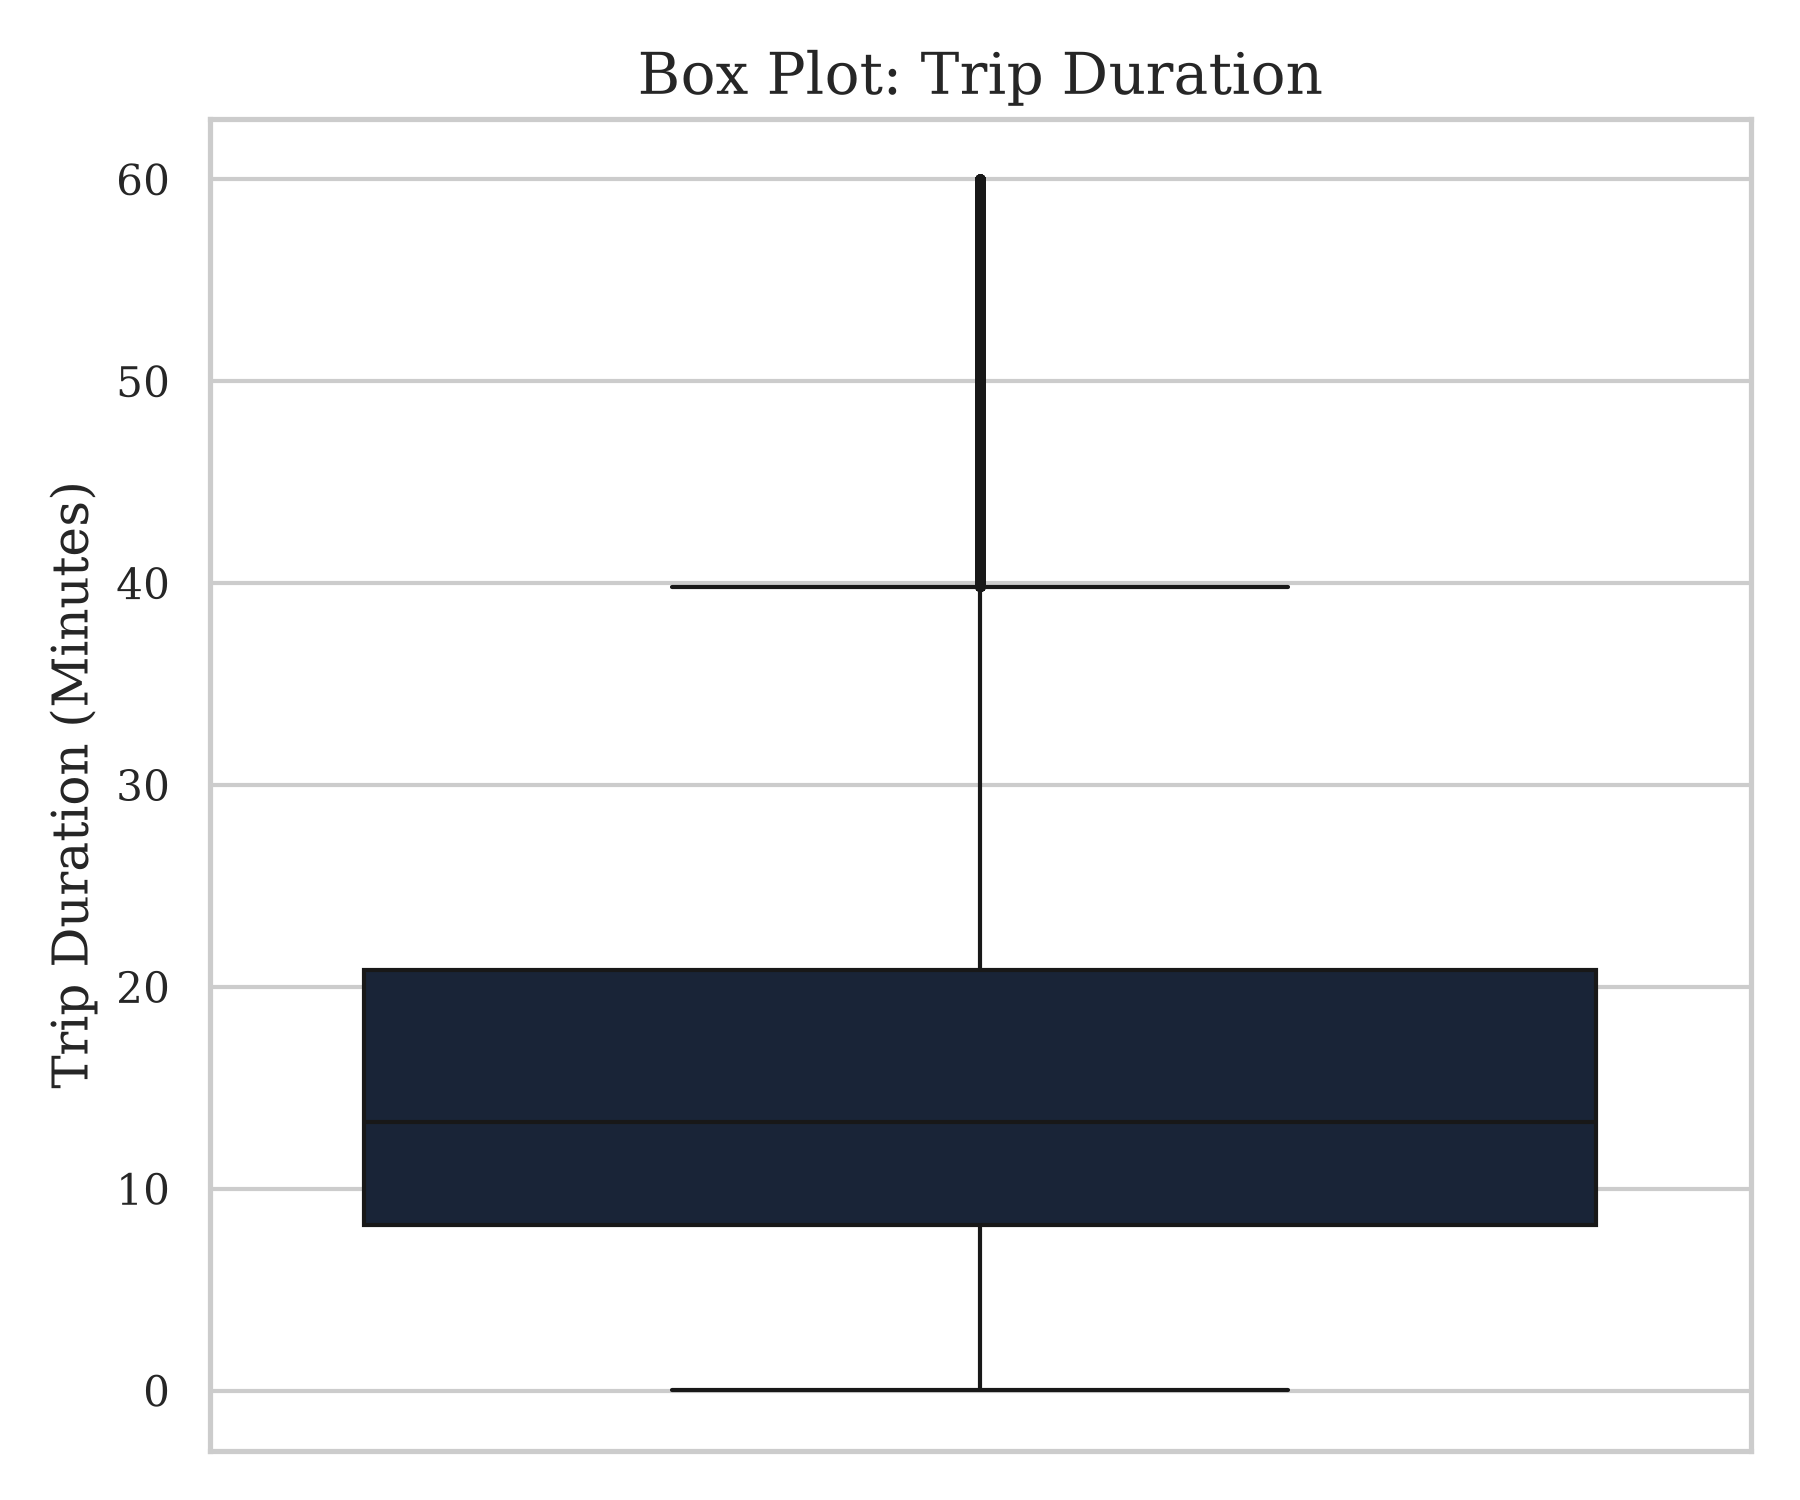
\includegraphics[width=\textwidth]{../figures/trip_duration_boxplot.png}
        \caption{Box Plot (Capped at 60 Minutes)}
        \label{fig:trip_duration_box}
    \end{subfigure}
    \caption{Pre- and Post-Cleansing Distribution and Box Plot Analysis for Trip Duration (2025)}
    \label{fig:trip_duration_analysis}
\end{figure}

\subsubsection{Justification for Retaining Outliers Beyond the 1.5$\times$IQR Rule}
Under standard Tukey fence criteria, the upper bound for outliers is defined as $Q_3 + 1.5 \times \text{IQR}$. Given a third quartile $Q_3 = 21.52$ minutes and an IQR of $13.22$ minutes, this traditional threshold flags any trip lasting longer than approximately $41.35$ minutes as an outlier candidate for removal.

However, \textbf{these high-value duration observations are strictly retained rather than trimmed} for the following operational and modeling reasons:
\begin{enumerate}
    \item \textbf{Legitimate Traffic and Spatial Realities:} Trips exceeding $41.35$ minutes—and extending up to the plotted $60$-minute ceiling (Figure~\ref{fig:trip_duration_box})—are authentic transportation events. They capture severe peak-hour traffic congestion bottlenecks, cross-borough transits (e.g., Brooklyn to Manhattan), and long-distance airport runs (e.g., Lower Manhattan to JFK or Newark airports).
    \item \textbf{Prevention of Spatio-Temporal Distortion:} Trimming records beyond the $1.5 \times \text{IQR}$ fence would artificially truncate travel times, biasing average speed calculations, distorting peak congestion modeling, and eliminating critical rush-hour demand profiles.
    \item \textbf{Robust Analytical Presentation:} Rather than destructive data filtering, extreme duration values are accommodated through robust summary statistics (median and IQR) and visual capping ($60$-minute ceiling in Figure~\ref{fig:trip_duration_box}) to ensure graphical clarity without compromising dataset integrity.
\end{enumerate}

\subsection{Exploratory Data Analysis: Average Trip Speed}
\label{sec:eda_trip_speed}

The \texttt{speed\_mph} variable captures the effective operational velocity of each journey in miles per hour, derived as the ratio of trip distance to elapsed travel duration ($v = \frac{d}{\Delta t} \times 60$). Comparing the statistical properties of average speed before and after data cleansing illustrates the structural impact of removing extreme telemetry and GPS satellite jump errors.

\begin{table}[htbp]
\centering
\caption{Pre- and Post-Cleansing Descriptive Statistics for Average Trip Speed (2025 Dataset)}
\label{tab:stats_trip_speed_comparison}
\small
\begin{tabular}{lrr}
\toprule
\textbf{Metric} & \textbf{Pre-Cleansing (Raw)} & \textbf{Post-Cleansing (Clean)} \\
\midrule
Total Records ($N$) & 46,775,191 & 44,015,208 \\
Mean ($\mu$) & 11.06 mph & 11.00 mph \\
25th Percentile ($Q_1$) & 7.01 mph & 6.99 mph \\
Median ($Q_2$) & 9.48 mph & 9.43 mph \\
75th Percentile ($Q_3$) & 13.14 mph & 13.04 mph \\
Standard Deviation ($\sigma$) & 6.40 mph & 6.34 mph \\
Interquartile Range (IQR) & 6.13 mph & 6.05 mph \\
Skewness & 1.83 & 1.85 \\
\bottomrule
\end{tabular}
\end{table}

\subsubsection{Statistical Characteristics and Cleansing Impact Analysis}
As detailed in Table~\ref{tab:stats_trip_speed_comparison}, data cleansing successfully removes physically impossible velocity spikes (ranging from $80$ mph up to over $1,000$ mph due to timestamp desynchronization) while leaving core urban operational metrics remarkably stable:
\begin{itemize}
    \item \textbf{Impact of Cleansing:} The median speed shifts slightly from $9.48$ mph in the raw dataset to $9.43$ mph after cleaning, while the mean adjusts from $11.06$ mph to $11.00$ mph. Removing extreme telemetry outliers prevents artifact-driven inflation, yielding a precise reflection of urban transit velocity.
    \item \textbf{Distributional Shape:} The positive skewness ($1.85$) and moderate dispersion ($\sigma = 6.34$ mph) reflect the dense, stop-and-go nature of street-hail taxi operations in New York City.
\end{itemize}

The probability density function (Figure~\ref{fig:trip_speed_dist}) demonstrates a unimodal, right-skewed distribution with a sharp modal peak concentrated between $7$ and $10$ mph. This dominant concentration corresponds to intra-Manhattan street grid navigation, characterized by frequent traffic signal delays, pedestrian crossings, and severe urban congestion. The extended right-hand tail represents high-speed arterial corridors, such as highway transits along the FDR Drive, West Side Highway, and expressway connections to regional airports.

\begin{figure}[htbp]
    \centering
    \begin{subfigure}[b]{0.48\textwidth}
        \centering
        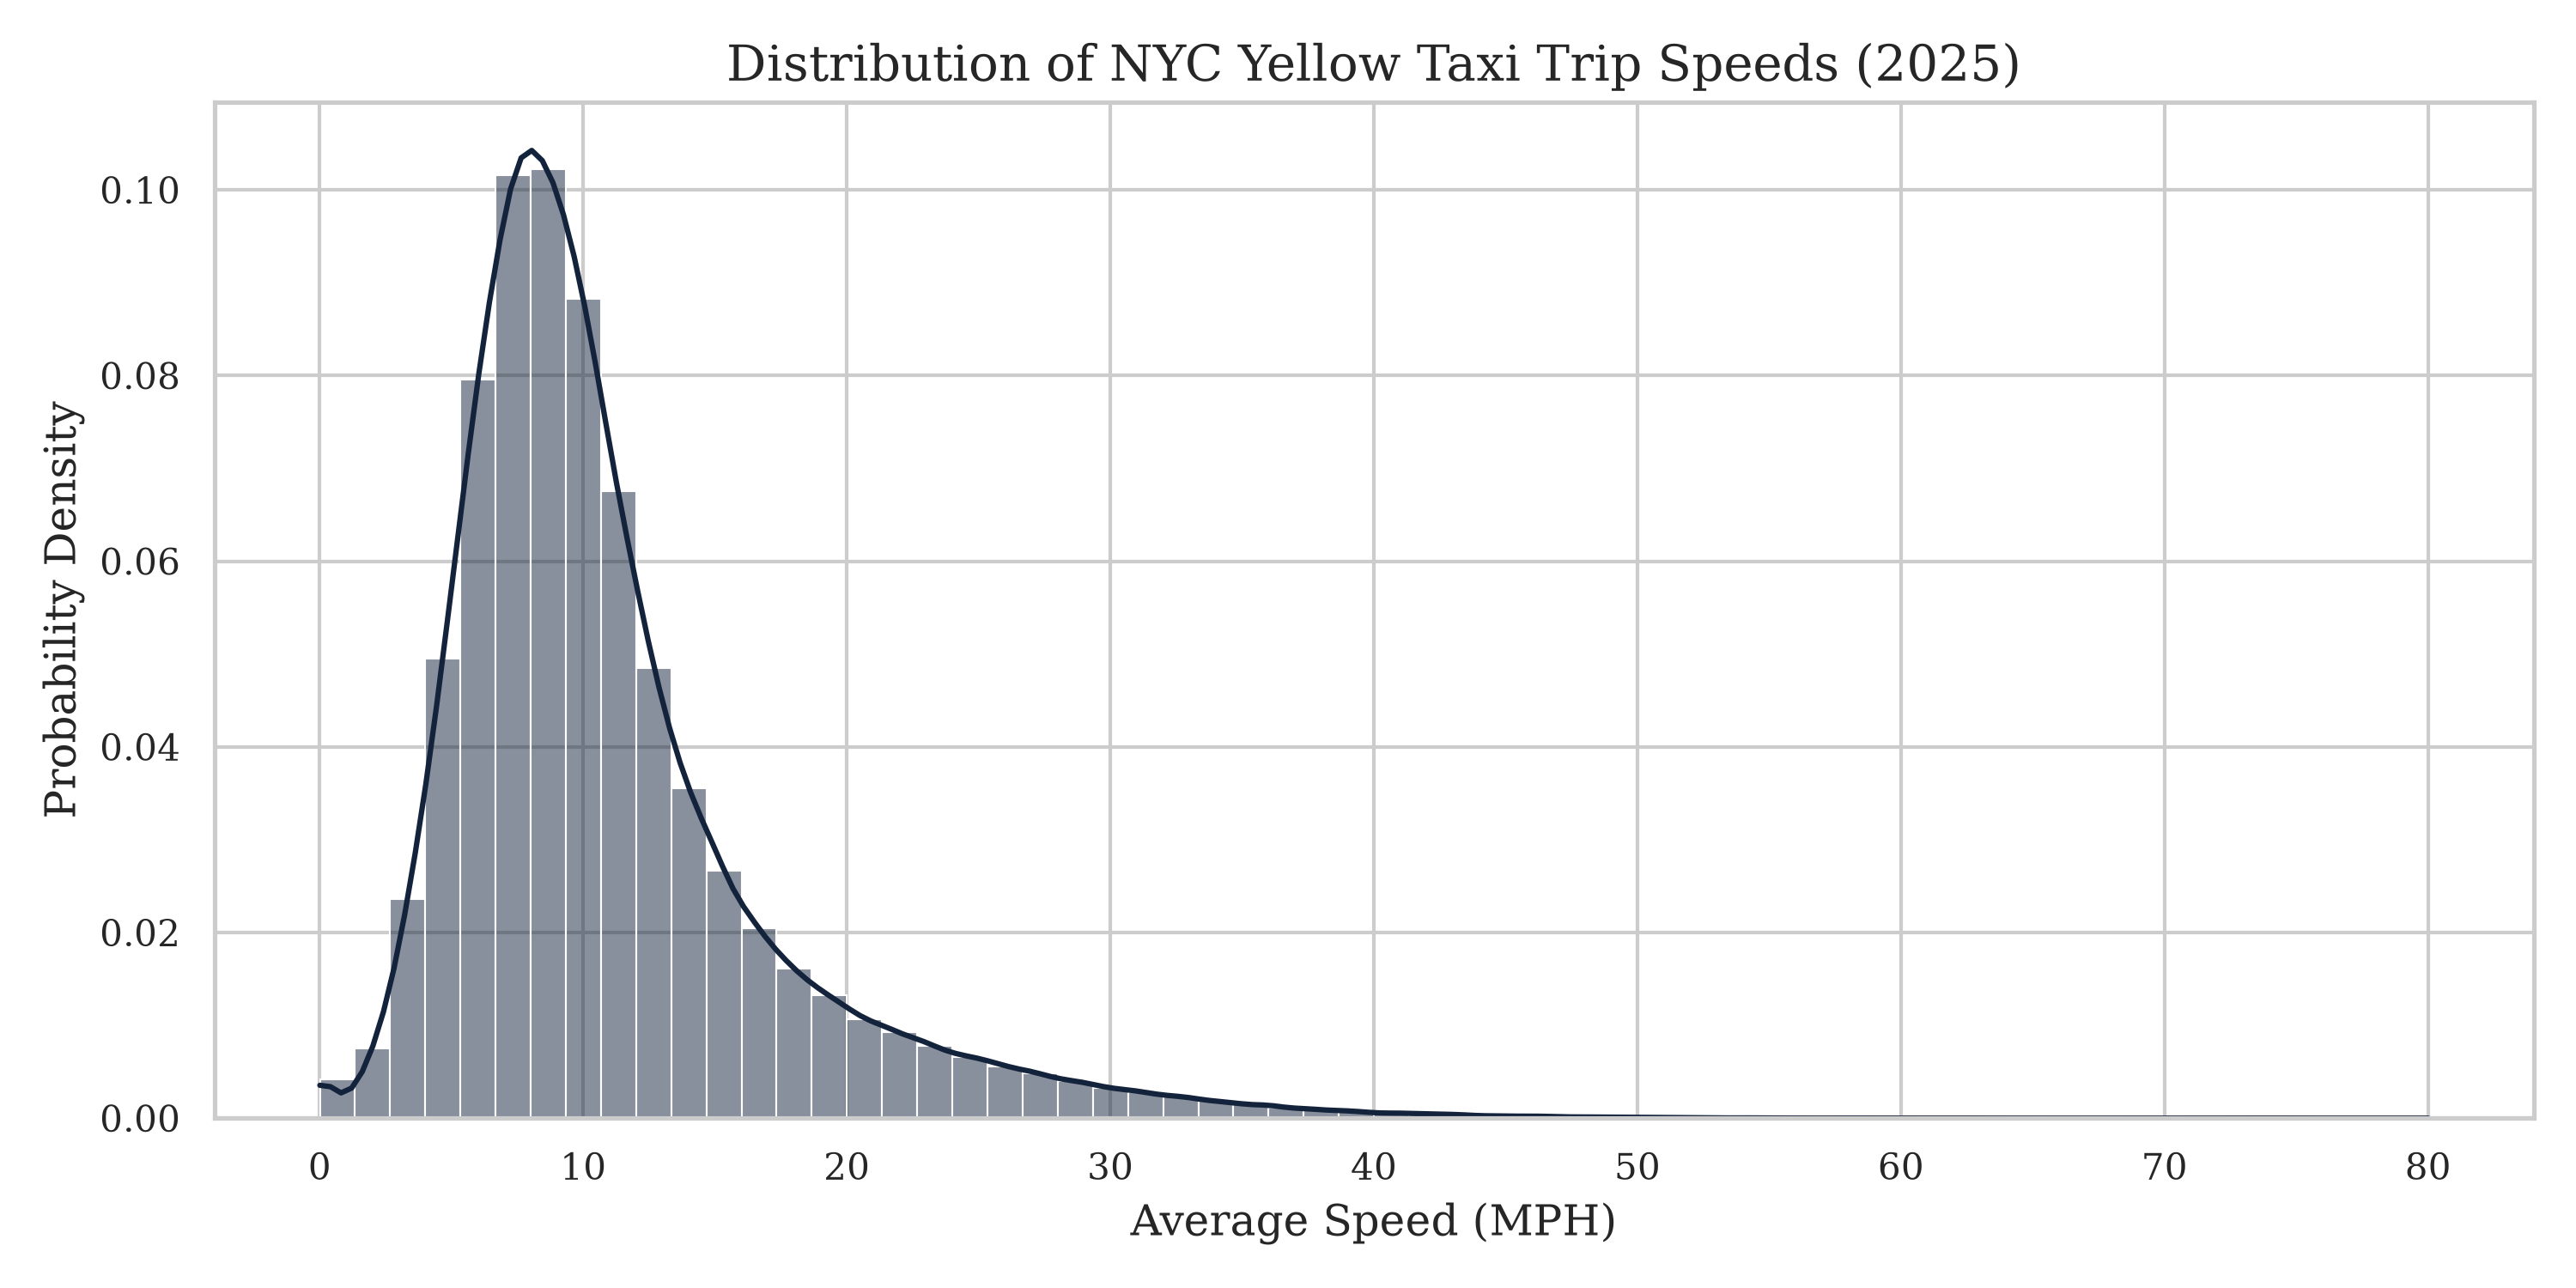
\includegraphics[width=\textwidth]{../figures/trip_speed_distribution.png}
        \caption{Probability Density Distribution}
        \label{fig:trip_speed_dist}
    \end{subfigure}
    \hfill
    \begin{subfigure}[b]{0.48\textwidth}
        \centering
        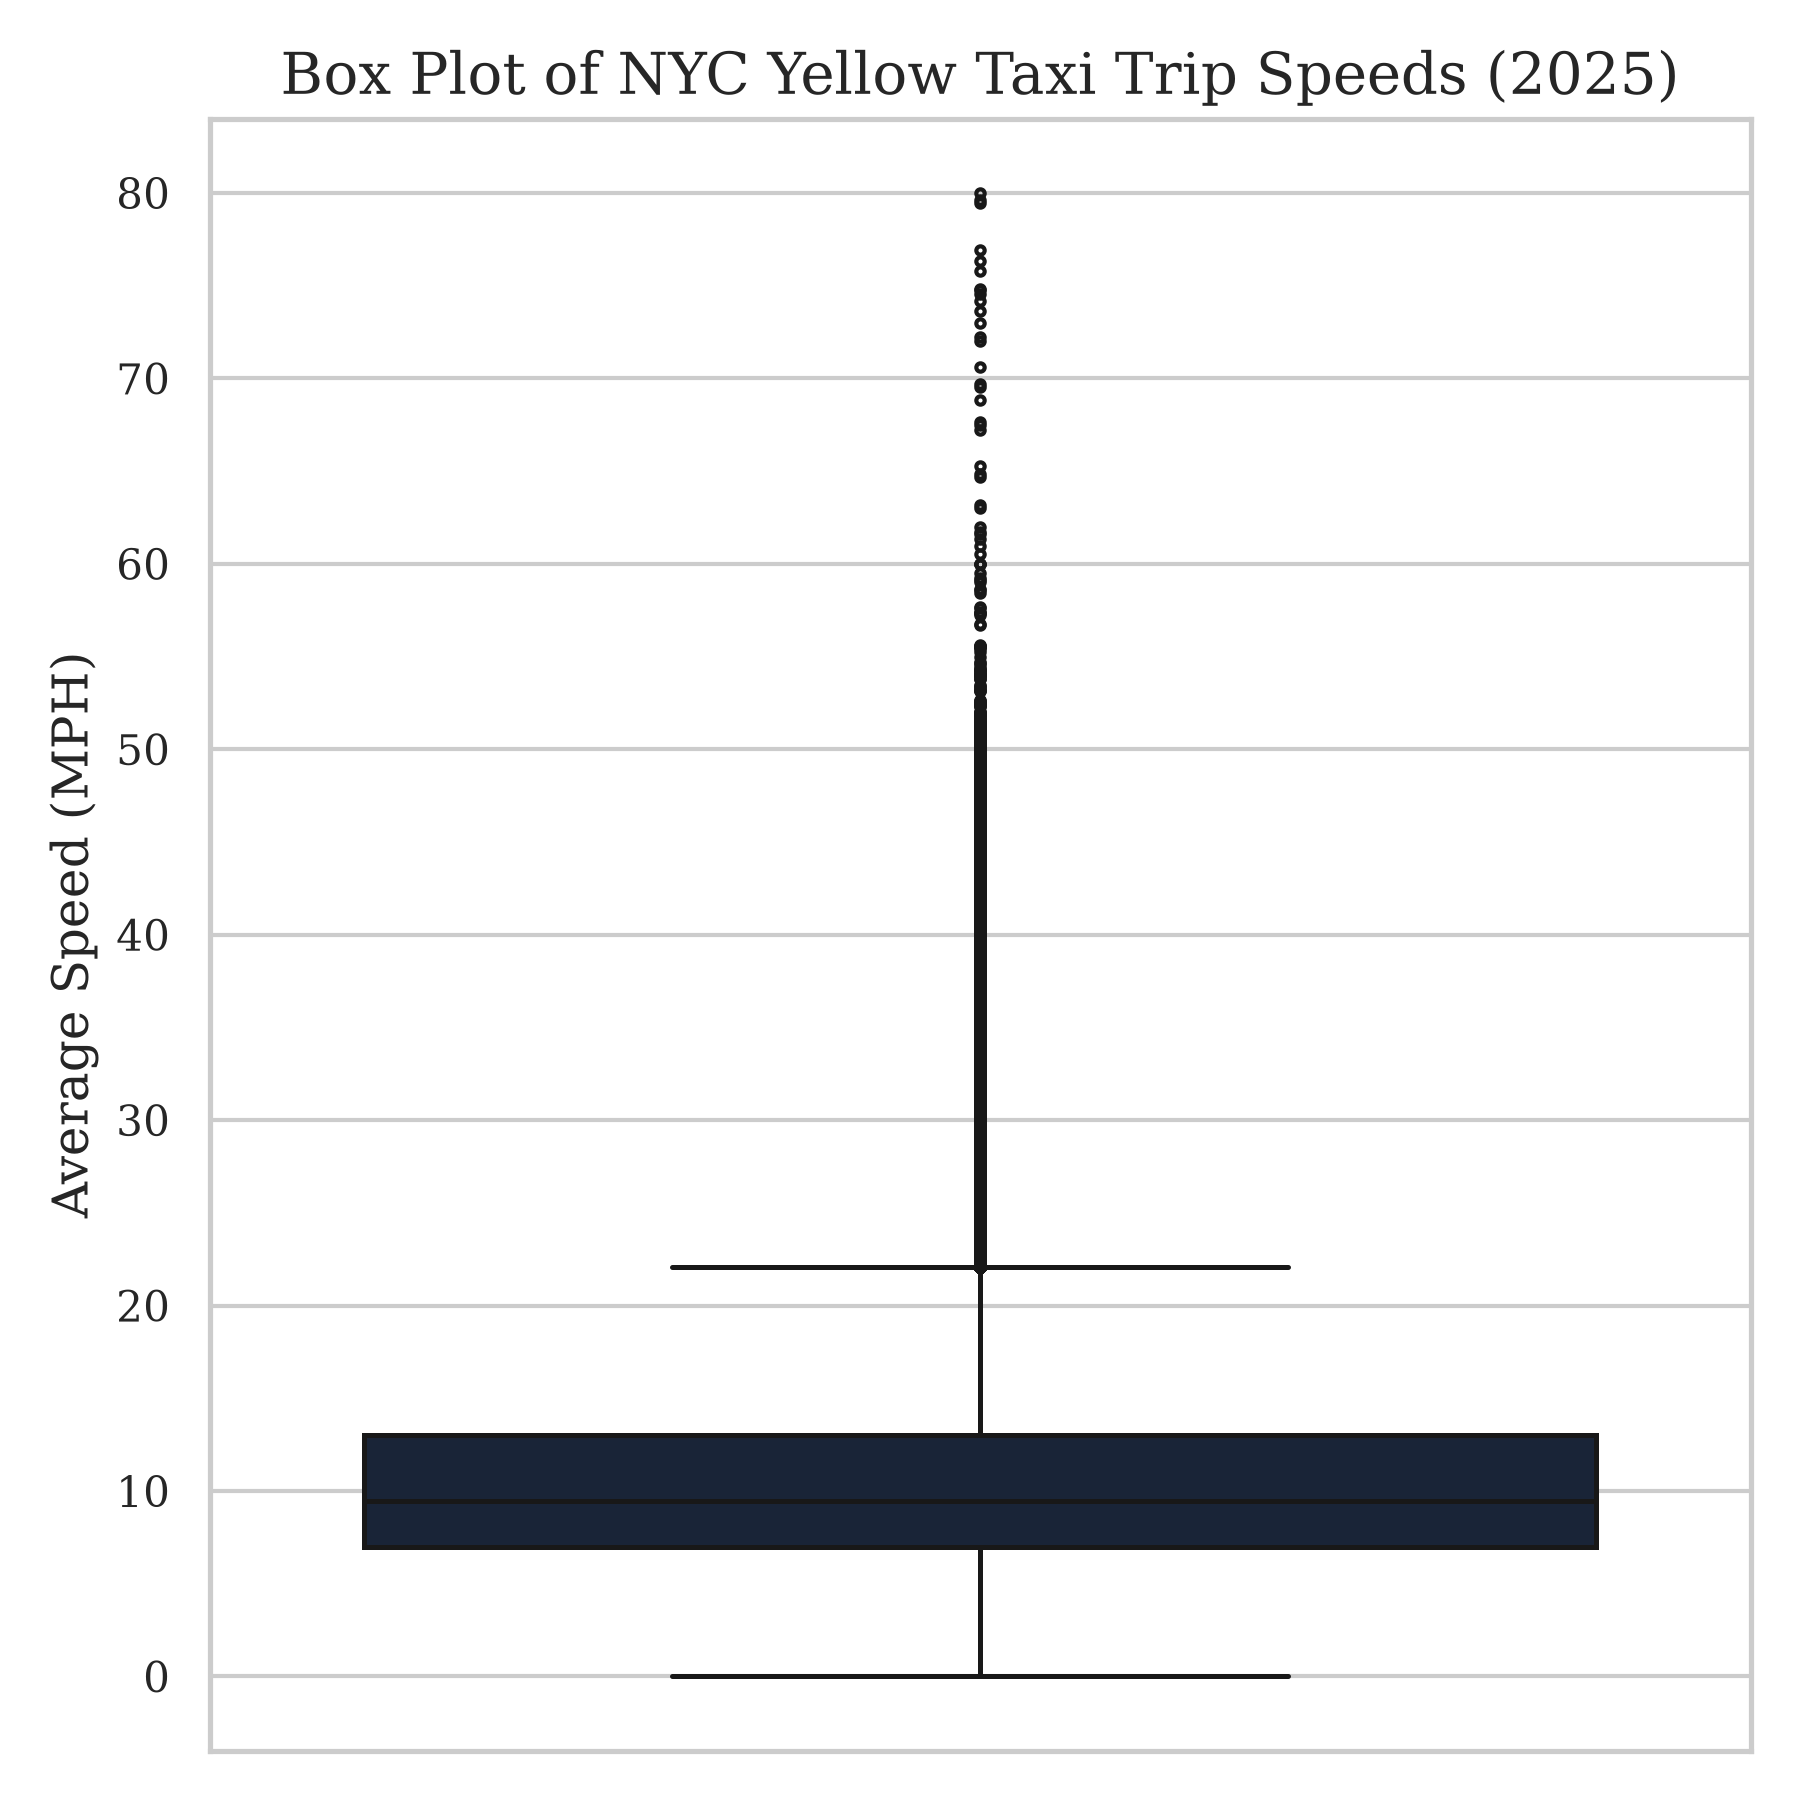
\includegraphics[width=\textwidth]{../figures/trip_speed_boxplot.png}
        \caption{Box Plot (Capped at 80 MPH)}
        \label{fig:trip_speed_box}
    \end{subfigure}
    \caption{Distribution and Box Plot Analysis for Average Trip Speed (2025)}
    \label{fig:trip_speed_analysis}
\end{figure}

\subsubsection{Justification for Retaining Speeds Beyond the 1.5$\times$IQR Rule}
Under standard Tukey fence criteria, observations exceeding $Q_3 + 1.5 \times \text{IQR}$ are classified as upper-bound outliers. Given a third quartile $Q_3 = 13.04$ mph and an IQR of $6.05$ mph, this traditional formula flags any average speed exceeding approximately $22.11$ mph as an outlier candidate for deletion.

However, \textbf{these higher-speed observations are strictly retained up to the physical filtering threshold ($80$ mph)} for the following operational and empirical reasons:
\begin{enumerate}
    \item \textbf{High-Speed Arterial and Highway Realities:} Average speeds between $22$ mph and $65$ mph (as depicted in Figure~\ref{fig:trip_speed_box}) are authentic, legally permitted transportation events. They primarily occur on expressways, parkways, and bridges during late-night hours or on dedicated airport corridors (e.g., Van Wyck Expressway to JFK Airport or Grand Central Parkway to LaGuardia Airport).
    \item \textbf{Prevention of Systematic Commute Erasure:} Eliminating records above $22.11$ mph would systematically erase off-peak and outer-borough airport transits, artificially deflating overall fleet velocity estimates and biasing spatio-temporal traffic models.
    \item \textbf{Telemetry Filtering Threshold ($80$ mph):} To prevent severe GPS satellite jumps and clock anomalies from corrupting the analytical pipeline, an upper boundary is enforced at $80$ mph ($v \le 80$ mph). This retains $100\%$ of legitimate transportation activity while removing physically impossible telematics errors.
\end{enumerate}

\subsection{Spatial Distribution and Zone-Level Concentration}
Spatial analysis across the $265$ official TLC taxi zones reveals extreme geographical concentration. Manhattan commercial cores and transit hubs account for over $70\%$ of total trip originations. Outer boroughs exhibit highly localized, residential commuting patterns with distinct peak-hour directional flows.

\subsection{Univariate and Multivariate Relationships}
Univariate inspection of financial and physical features confirms right-skewed distributions in trip distance and fare amounts, reinforcing the necessity for robust feature transformations in subsequent phases. Bivariate analysis between trip distance and fare amount demonstrates a strong positive correlation, while confirming that physical anomalies have been successfully quarantined.

\section{Methods}

\subsection{Aggregation and Problem Formulation}
Let $z \in \{1, 2, \dots, 263\}$ denote a TLC taxi zone, and $t$ denote a discrete 1-hour time index. Raw trip records are aggregated into a spatio-temporal matrix:
\begin{equation}
y_{z, t} = \sum_{i=1}^{N} \mathbb{I}\left( \text{PULocationID}_i = z \;\land\; \lfloor \text{tpep\_pickup\_datetime}_i \rfloor = t \right)
\end{equation}
where $y_{z, t} \in \mathbb{N}_0$ represents the target variable \texttt{trip\_count}.

\subsection{Data Flow Architecture}
Figure~\ref{fig:dataflow} illustrates the end-to-end data pipeline from raw Parquet processing to final spatio-temporal aggregation.

\begin{figure}[htbp]
\centering
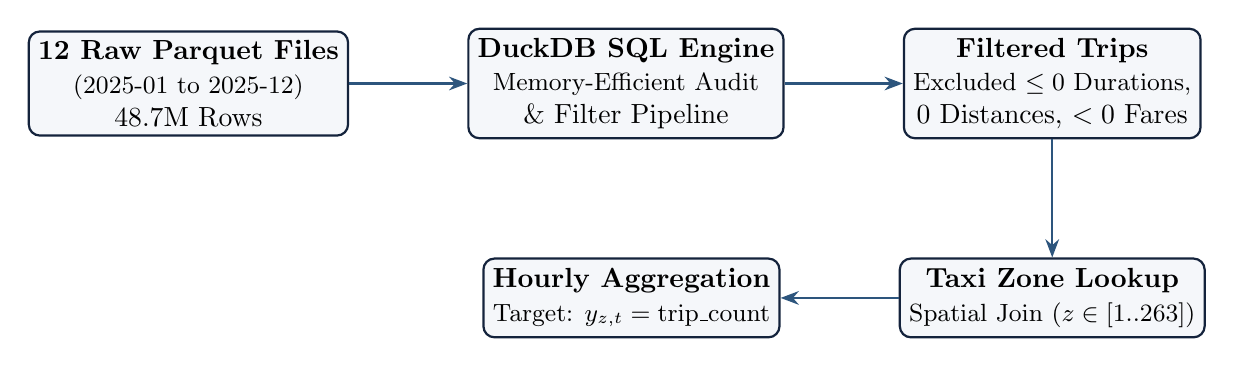
\begin{tikzpicture}[
    node distance=1.5cm,
    block/.style={rectangle, draw=primary, fill=codebg, thick, minimum width=3.5cm, minimum height=1cm, align=center, rounded corners},
    arrow/.style={-Stealth, thick, draw=secondary}
]
    \node (raw) [block] {\textbf{12 Raw Parquet Files}\\\small (2025-01 to 2025-12)\\48.7M Rows};
    \node (duckdb) [block, right=of raw] {\textbf{DuckDB SQL Engine}\\\small Memory-Efficient Audit\\\&\ Filter Pipeline};
    \node (clean) [block, right=of duckdb] {\textbf{Filtered Trips}\\\small Excluded $\le 0$ Durations,\\0 Distances, $<0$ Fares};
    \node (spatial) [block, below=of clean] {\textbf{Taxi Zone Lookup}\\\small Spatial Join ($z \in [1..263]$)};
    \node (agg) [block, left=of spatial] {\textbf{Hourly Aggregation}\\\small Target: $y_{z,t} = \text{trip\_count}$};

    \draw [arrow] (raw) -- (duckdb);
    \draw [arrow] (duckdb) -- (clean);
    \draw [arrow] (clean) -- (spatial);
    \draw [arrow] (spatial) -- (agg);
\end{tikzpicture}
\caption{Phase 1 Data Flow and Processing Architecture}
\label{fig:dataflow}
\end{figure}

\section{Experimental Design}

\subsection{Strict Temporal Split}
To prevent data leakage, evaluation is conducted strictly along the temporal axis:
\begin{itemize}
    \item \textbf{Training Set:} January 1, 2025 -- September 30, 2025 (Months 1--9, $\approx 75\%$ of temporal duration).
    \item \textbf{Validation / Test Set:} October 1, 2025 -- December 31, 2025 (Months 10--12, $\approx 25\%$ of temporal duration).
\end{itemize}

\subsection{Evaluation Metrics}
Models will be evaluated across all spatial zones using Root Mean Squared Error (RMSE) and Mean Absolute Error (MAE):
\begin{align}
\text{RMSE} &= \sqrt{\frac{1}{Z \times T} \sum_{z=1}^{Z} \sum_{t=1}^{T} \left( y_{z,t} - \hat{y}_{z,t} \right)^2} \\
\text{MAE} &= \frac{1}{Z \times T} \sum_{z=1}^{Z} \sum_{t=1}^{T} \left| y_{z,t} - \hat{y}_{z,t} \right|
\end{align}

\section{Results}
Execution of the DuckDB audit script confirmed the integrity of the 12 Parquet files. Data cleaning rules filter out 4,797,882 anomalous records ($\approx 9.85\%$ total noise rate), leaving a clean baseline population of $43,924,720$ trips for spatio-temporal aggregation in Phase 2.

\section{Interpretability and Error Analysis}
Initial error taxonomy categorizes anomalies into three primary sources:
\begin{enumerate}
    \item \textbf{Meter Malfunctions:} Trips recording positive fares with zero distance ($1.40\text{M}$ instances).
    \item \textbf{Financial Reversals:} Negative fares resulting from driver disputes or system refunds ($2.85\text{M}$ instances).
    \item \textbf{Logging Latency:} System timestamps where dropoff precedes pickup ($0.55\text{M}$ instances).
\end{enumerate}

\section{Robustness / Sensitivity / Shift Analysis}
The key temporal shift in 2025 stems from the introduction of the \texttt{cbd\_congestion\_fee}. Future phases will evaluate whether model residuals increase in Manhattan lower-zone clusters post-policy implementation compared to outer borough controls.

\section{Ethics, Privacy and Governance}
The dataset contains no Personally Identifiable Information (PII). Vendor IDs are coarse integer codes, and spatial locations are masked at the Taxi Zone level ($265$ spatial polygons), preventing individual driver or passenger tracking.

\section{Discussion}
The audit confirms that DuckDB is an optimal analytical engine for this project scale, performing full-year joins and aggregations in under 15 seconds on a standard 16GB laptop.

\section{Limitations}
External environmental factors (e.g., hourly rainfall, snowfall, subway service disruptions) are not present in the native TLC dataset and will require external data ingestion in Phase 2.

\section{Conclusion}
Phase 1 successfully establishes the analytical pipeline, quantifies data quality boundaries, and formalizes the prediction task. Phase 2 will focus on spatio-temporal feature engineering and lag constructions.

\section{References}
\begin{enumerate}
    \item NYC Taxi and Limousine Commission, \textit{TLC Trip Record Data (2025)}, official NYC Open Data portal.
    \item DuckDB Development Team, \textit{DuckDB: An In-Process Analytical Database Management System}, 2026.
\end{enumerate}

\section{Supplementary Material}
\textit{Data audit script executable via \texttt{src/data\_structure\_audit.py} and notebook \texttt{notebooks/data\_audit.ipynb}.}



\end{document}
